\chapter{The search for standard model~\tttt production in \runone at $\sqrt{s} =$ 8TeV }
\label{c:Run1}

\section{Introduction}
In this chapter, an analysis of the full 2012 CMS dataset at $\sqrt{s} =$ 8TeV with 19.7 \fbinv of data is presented where the Standard Model production of four top quarks (\tttt) is sought. Standard model \tttt production has a cross section of $\sigmattttSM \approx 1.3$ fb at NLO with NNLO corrections~\cite{Barger201070,Bevilacqua2012}. 

% this equates to approximately 26 events in the 2012 dataset in all decay channels. However, in this analysis, only final states where one of the top quarks decays leptonically into an electron or muon are considered. These are referred to as the single lepton channels and they are the most prevalent decay mode as can be seen in ~\fxnote*{add fig}{figX}. One of the main challenges of this analysis is to distinguish this extremely rare signal process with the overwhelmingly large background process of top-pair production (\ttbar) which is five orders of magnitude greater than the \tttt signal process, the latest measurement putting it at $241.5 \pm 8.5$ \pbinv ~\cite{CMS-PAS-TOP-14-016}. 


%This analysis proceeds as follows; Section~\ref{sec:sigback} discuss the \tttt signal processes and the relevant background and Section~\ref{sec:datasimulation} describes the datasets and simulations of the signal and backrgound used. Section~\ref{sec:baseline} details the initial requirements imposed on the signal region while Section~\ref{sec:Calibrations} describes the calibrations made to the correct the simulation. The multi-jet background estimation is described in Section~\ref{sec:QCDbackground} and the multi-variate techniques used to increase the discrimination power between signal and background are contained in~\ref{sec:discriminating}. Discussion of the systematic uncertainties and extraction of the limit on the \tttt cross section are in Sections~\ref{sec:uncertainties} and~\ref{sec:limit}. Validation of the analysis can be found in Section~\ref{sec:signalinjection}. Finally, a summary and discussion of the ATLAS \tttt cross section limit can be found in Sections~\ref{sec:summary} and~\ref{sec:ATLASresult}.
Sections~\ref{sec:QCDbackground},~\ref{sec:njetcatlimit} and~\ref{sec:signalinjection} are the authors personal contribution to the analysis.

%An initial baseline selection of requirements on the number of leptons, jets, b-tagged jets, transverse hadronic energy (\HT) and transverse missing energy (\MET) reduces the \ttbar background to three orders of magnitude greater than the \tttt signal. As \ttbar remains a very large background, multi-variate techniques are employed to reconstruct top quarks and then ultimately to find a discriminator value to distinguish between signal and background.
%In the absence of an excess of events over background, the \CLS method is used to obtain an observed limit on the cross section of \tttt production of 32 fb at 95\% confidence level compared to 32$\pm17$ fb expected.



\section{Data and Simulation}
\label{sec:datasimulation}
This analysis uses data from proton-proton collision at the CMS experiment in 2012 at $\sqrt{s}=8$~TeV.
For the muon (electron) channel, the data were collected using a trigger based on the presence of at least one muon (electron) candidate with $\pt > $ 24 (27) GeV and corresponds to an integrated luminosity of 19.7 \fbinv .
% The full 2012 SingleElectron dataset is used for the electron channel, which requires an electron candidate with $\pt > $ 27 GeV and corresponds to an integrated luminosity of 19.7 \fbinv.
The signal SM \tttt Monte Carlo (MC) samples and the background MC samples are given in table~\ref{tab:datasets_sim_8tev}, along with the MC generator used to produce these samples, the order at which they were produced and the number of events produced. MC samples were produced for the scale and matching systematics, these can be found in table~\ref{tab:datasets_sys_8tev}. In this analysis the scale uncertainty includes the ME scale and PS scale.


\begin{table}[ht!]
% \tiny
\centering
\begin{tabular}{| l | l | l | p{2cm} |}
 \hline 
 Dataset & Events & Generator & Order \\
\hline
TTTT & 100K & Madgraph  $+$ Tauola& O \\
\hline
TTJets\_SemiLeptMGDecays &25M & Madgraph $+$ Tauola & O \\
\hline
TTJets\_HadronicMGDecays &31M & Madgraph  $+$ Tauola& O \\
\hline
TTJets\_FullLeptMGDecays\ & 12M & Madgraph  $+$ Tauola& O \\
\hline
W4JetsToLNu & 13M & Madgraph & O \\
\hline
Tbar\_tW-channel & 500K & Powheg $+$ Tauola & O\\
\hline
T\_tW-channel & 500K & Powheg $+$ Tauola & O \\
\hline
T\_t-channel & 3.8M & Powheg $+$ Tauola & O \\
\hline
Tbar\_s-channel & 260K & Powheg $+$ Tauola & O \\
\hline
T\_s-channel & 139K & Powheg $+$ Tauola & O \\
\hline
Tbar\_t-channel & 2M  & Powheg $+$ Tauola & O \\
\hline
DY4JetsToLL & 6.2M & Madgraph & O  \\
\hline
DYJetsToLL & 6.7M & Madgraph & O \\
\hline
TTZJets  & 200K & Madgraph & O \\
\hline
TTWJets\ & 200K & Madgraph & O \\
\hline
TTH\_HToBB & 1M & Pythia6 $+$ Tauola & O \\
\hline
ZZ & 10M & Pythia6 $+$ Tauola & O \\
\hline
WZ &10M & Pythia6 $+$ Tauola & O \\
\hline
WW &10M & Pythia6 $+$ Tauola & O \\
\hline
\end{tabular}
 \caption{Dataset name, total number of events, MC generator and order of the simulated samples.}
  \label{tab:datasets_sim_8tev}
  \end{table}


\begin{table}[ht!]
% \tiny
\centering
\begin{tabular}{| l | l | l | p{2cm} |}
 \hline 
 Dataset & Events & Generator & Order \\
\hline
TTJets\_scaledown & 5M  & Madgraph $+$ Tauola & O \\
\hline
TTJets\_scaleup & 5M  & Madgraph $+$ Tauola & O \\
\hline
TTJets\_matchingdown & 5M & Madgraph $+$ Tauola & O  \\
\hline
TTJets\_matchingup & 5M & Madgraph $+$ Tauola & O \\
\hline
\end{tabular}
 \caption{Dataset name, total number of events, MC generator and order of the simulated systematic samples.}
  \label{tab:datasets_sys_8tev}
\end{table}

\section{Baseline Event Selection}
\label{sec:baseline}
To select \tttt events and suppress background events, a set of criteria is applied to the reconstructed objects in events which are triggered by the single muon or single electron triggers.
For the muon channel these are:
\begin{itemize}
\setlength\itemsep{0em}
\item Exactly one tight muon
\item Exactly zero additional loose muons
\item Exactly zero loose electrons
\item At least 6 jets with $\pt >$ 30 \GeV
\item At least 2 CSVM tagged b-jets
\item $\HT > $ 400 \GeV 
\item $\MET > $ 30 \GeV 
\end{itemize}
For the electron channel these are:
\begin{itemize}
\itemsep0em 
\item Exactly one tight electron
\item Exactly zero additional loose electrons
\item Exactly zero loose muons
\item At least 6 jets with $\pt >$ 30 \GeV
\item At least 2 CSVM tagged b-jets
\item $\HT > $ 400 \GeV 
\item $\MET > $ 30 \GeV 
\end{itemize}

\section{Corrections to the simulation}
\label{sec:Calibrations8}
All corrections are described in section~\ref{sec:Calibrations}.
The events for all background and signal samples which pass the baseline event selection are given a weight which is the product of the weight for the pile up corrections, a weight to correct the b-tag modelling from the method in ~\ref{subsec:method1btag} and a weight for lepton modelling corrections. The heavy flavour jet modelling from section~\ref{ttbbmod} is applied to the \ttbar background.



% \subsection{b tag modelling}

% There are significant differences between b tag efficiencies measured by CMS in data and the efficiencies as measured in simulation. To account for this, a weight must be applied applied to the selected MC events in order to predict the correct event yield in data. The full method can be found in this reference~\cite{CMS-PAS-BTV-13-001}.

% \subsection{Heavy flavour jet modelling}

% There is a discrepancy between data and simulation in the tails of the \fxnote*{show unweighted}{distribution} of the number of b-tagged jets (\nbtags) which suggests that the amount of heavy flavour jets in \ttbar events is incorrectly simulated. The ratio of \heavyflavour was measured by CMS to be $2.2 \pm 0.3 \left( \textrm{stat.} \right) \pm 0.5 \left(\textrm{sys.} \right)\% $ ~\cite{CMS:2014yxa} at $\sqrt{s} =$ 8TeV. To incorporate this ratio into the analysis, the MC truth information of the \ttbar$+$jets MC sample is used to split the sample into \ttbb, \ttcc and \ttll, where l denotes light quarks and gluons (\cPqu, \cPqd, \cPqs, \cPg) . Weights are applied to each sub-sample to match the measured ratio whilst preserving the total number of \ttbar events. After this procedure is applied, the agreement between data and simulation in the \nbtags distribution is improved as can be seen in Fig~\ref{fig:datasimnbtags}.

% \subsection{Lepton modelling}
% Due to a difference between data and simulation in the efficiency of lepton identification and isolation, a weight is applied to events which is dependent on the selected leptons $\eta$, $\pt$ and lepton flavour.
\section{Weighted event counts through baseline event selection \label{cutflow}}

The event counts weighted by the various corrections in section~\ref{sec:Calibrations8} are given for the muon (electron) channel in table~\ref{tab:museltable8} (table~\ref{tab:eseltable8}). It is quite evident that the main background is \ttbar production, with smaller contributions coming from W$+$jets, Z$+$jets and single top (ST) as well as almost negligible contributions from the diboson and TT+X background (X $=$ H, Z, W).
\fxnote {discuss grouping of backgrounds}




\begin{table}
\tiny
\caption{Cut flow for the $\mu$ + jets channel ($19695.0~pb^{-1}$ of int. lumi.)}
\label{tab:museltable8}
\centering
\begin{tabular}{|c|c|c|c|c|c|c|c|c|c|c|c|c|}
\hline
&$Data$ &$\tttt$  &$ttH$  &$Wjets$ &$Zjets$ &$ST$ &$WW$ &$WZ$ &$ZZ$ &$TTZ$  &$TTW$  &$\ttbar$ \\
\hline
Trigger&  120508.0  &4.5  &171.8  &16094  &3916.3 &3256.2 &272.0  &161.1  &71.5 &219.3  &277.5  &84476  \\

1 iso. $\mu$& 95723.0 &3.5  &141.6  &13655  &2635.1 &2750.2 &232.7  &125.0  &47.6 &168.5  &229.3  &70030  \\

Loose $\mu$ veto& 93385.0 &3.2  &138.9  &13654  &1835.3 &2739.2 &232.3  &114.7  &34.0 &153.5  &222.9  &69503  \\

Loose e veto& 91546.0 &2.5  &132.6  &13593  &1812.0 &2691.6 &228.9  &113.0  &33.3 &143.6  &206.0  &68040  \\

$>$= 6 Jets&  24791.0 &2.3  &59.1 &2428.4 &350.7  &591.9  &41.5 &20.0 &5.1  &71.8 &94.1 &21197  \\

$>$= 2 b-tags&  9260.0  &1.7  &46.0 &68.8 &15.2 &215.5  &3.1  &1.4  &0.6  &35.0 &39.5 &9138.8 \\

HT $>$=  400 GeV& 6342.0  &1.6  &37.7 &49.3 &10.4 &156.9  &2.6  &1.0  &0.4  &29.6 &32.8 &6542.2 \\

\MET $>$=  30 GeV&      5215.0  &1.5    &31.7   &41.5   &7.1    &132.2  &2.2    &0.9    &0.1    &24.4   &28.3   &5415.1 \\
\hline
\end{tabular}
\end{table}



\begin{table}
\tiny
\caption{Cut flow for the $e$ + jets channel ($19721.7~pb^{-1}$ of int. lumi.)}
\label{tab:eseltable8}
\centering
\begin{tabular}{|c|c|c|c|c|c|c|c|c|c|c|c|c|c|}
\hline
&$Data$ &$\tttt$  &$ttH$  &$Wjets$ &$Zjets$ &$ST$  &$WW$ &$WZ$ &$ZZ$ &$TTZ$  &$TTW$  &$\ttbar_{other}$ &$\ttbar_{semi-lep}$  \\
\hline
Trigger and PV& $1128500$ &$8.6$  &$307.8$  &$28831$  &$25118.7$  &$6494.4$ &$683.8$  &$464.1$  &$228.3$  &$440.4$  &$545.5$  &$14569$  &$157087$ \\

1 iso. e& $103856$  &$3.2$  &$117.6$  &$9631.6$ &$7183.4$ &$2212.4$ &$217.6$  &$136.8$  &$60.9$ &$156.4$  &$207.4$  &$5050$ &$59293$  \\

Loose e veto& $100861$  &$3.0$  &$115.9$  &$9611.2$ &$5354.2$ &$2199.2$ &$216.4$  &$121.7$  &$43.7$ &$144.7$  &$201.9$  &$4611$ &$59201$  \\

Loose mu veto&  $99402$ &$2.3$  &$110.9$  &$9605.0$ &$5340.7$ &$2172.0$ &$215.2$  &$120.8$  &$43.3$ &$134.4$  &$186.3$  &$3456$ &$59128$  \\

$>$= 6 Jets&  $26508$ &$2.1$  &$55.2$ &$1660.3$ &$1108.3$ &$490.7$  &$32.0$ &$20.6$ &$7.2$  &$67.6$ &$84.7$ &$977.8$  &$18799$  \\

$>$= 2 b-tags&  $8945$  &$1.5$  &$43.2$ &$45.4$ &$19.8$ &$179.3$  &$1.3$  &$2.0$  &$0.8$  &$31.5$ &$35.6$ &$421.1$  &$7941$ \\

HT $>$= 400 GeV&  $6278$  &$1.5$  &$35.6$ &$33.2$ &$13.9$ &$134.2$  &$1.0$  &$1.3$  &$0.5$  &$26.1$ &$29.1$ &$321.4$  &$5739.7$ \\

\MET $>$ 30 GeV & $5066$  &$1.3$  &$30.0$ &$25.4$ &$7.0$  &$114.2$  &$0.8$  &$1.1$  &$0.2$  &$21.5$ &$24.5$ &$297.0$  &$4676.9$ \\
\hline
\end{tabular}
\end{table}




\section{Data-simulation agreement}

% After the baseline event selection, events are weighted using the prescription for pile-up as described in Section~\ref{sec:pile-up}. The weights are applied for b-tagging, the heavy flavour jet modelling and the lepton modelling as described in Section~\ref{sec:run1:baseline}. 

The distributions which show the data-simulation agreement for \njets, \nbtags, \HT and \MET after these weights are applied are shown in Figs~\ref{fig:datasimnjets},~\ref{fig:datasimnbtags},~\ref{fig:datasimHT},~\ref{fig:datasimMET}. As the scale uncertainty is the largest uncertainty on the background, it is shown as a hatched error band on the distributions. It can be seen that there is good agreement between data and simulation in these distributions and that the signal (overlaid and multiplied by 100 for visibility) has a different shape in these variables in the background processes particularly in the \njets, \nbtags, \HT which make them viable candidates to be used in the event-level BDT.

\fxnote{Get version of plots from papers with bigger titles}

\begin{figure}[ht!]
\centering
    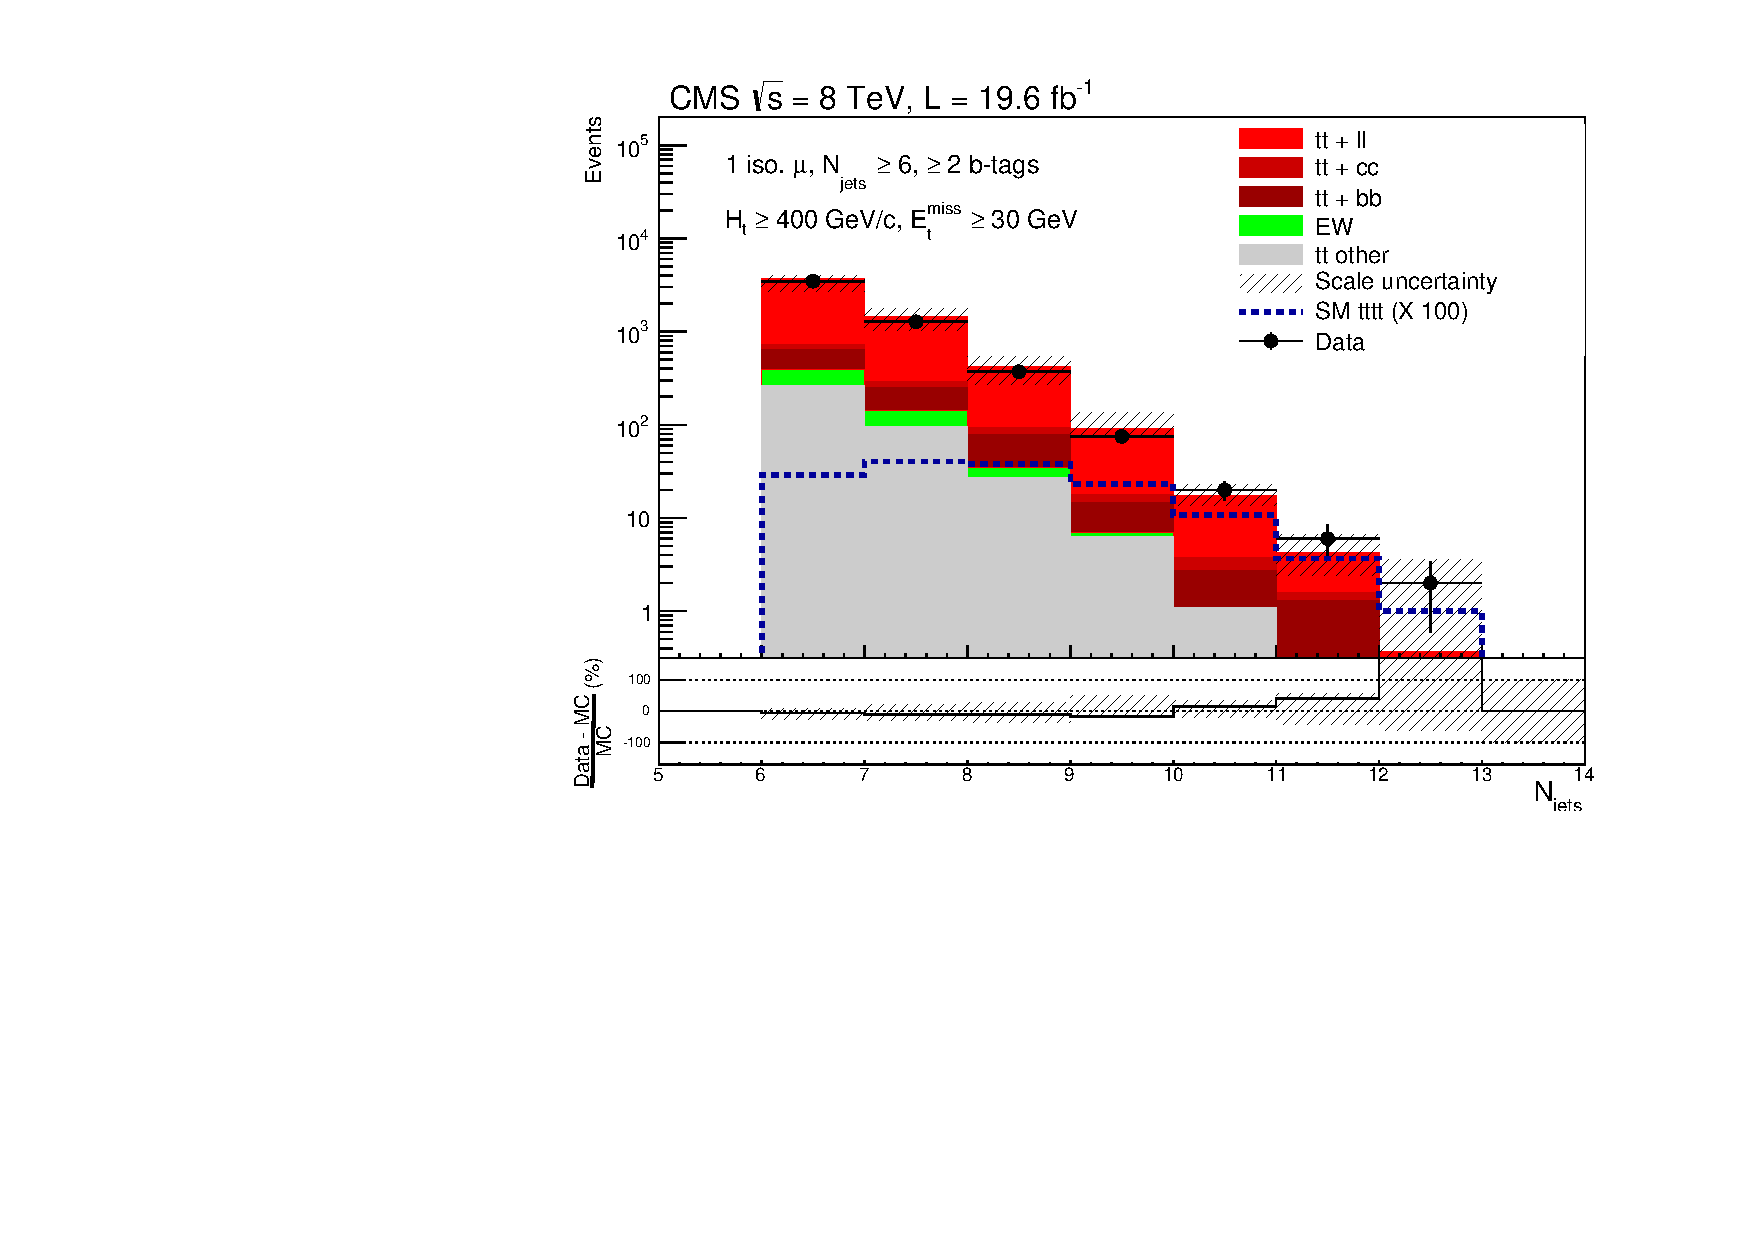
\includegraphics[width=0.49\textwidth]{images/Run1/NbOfSelectedJets_mu.pdf}
     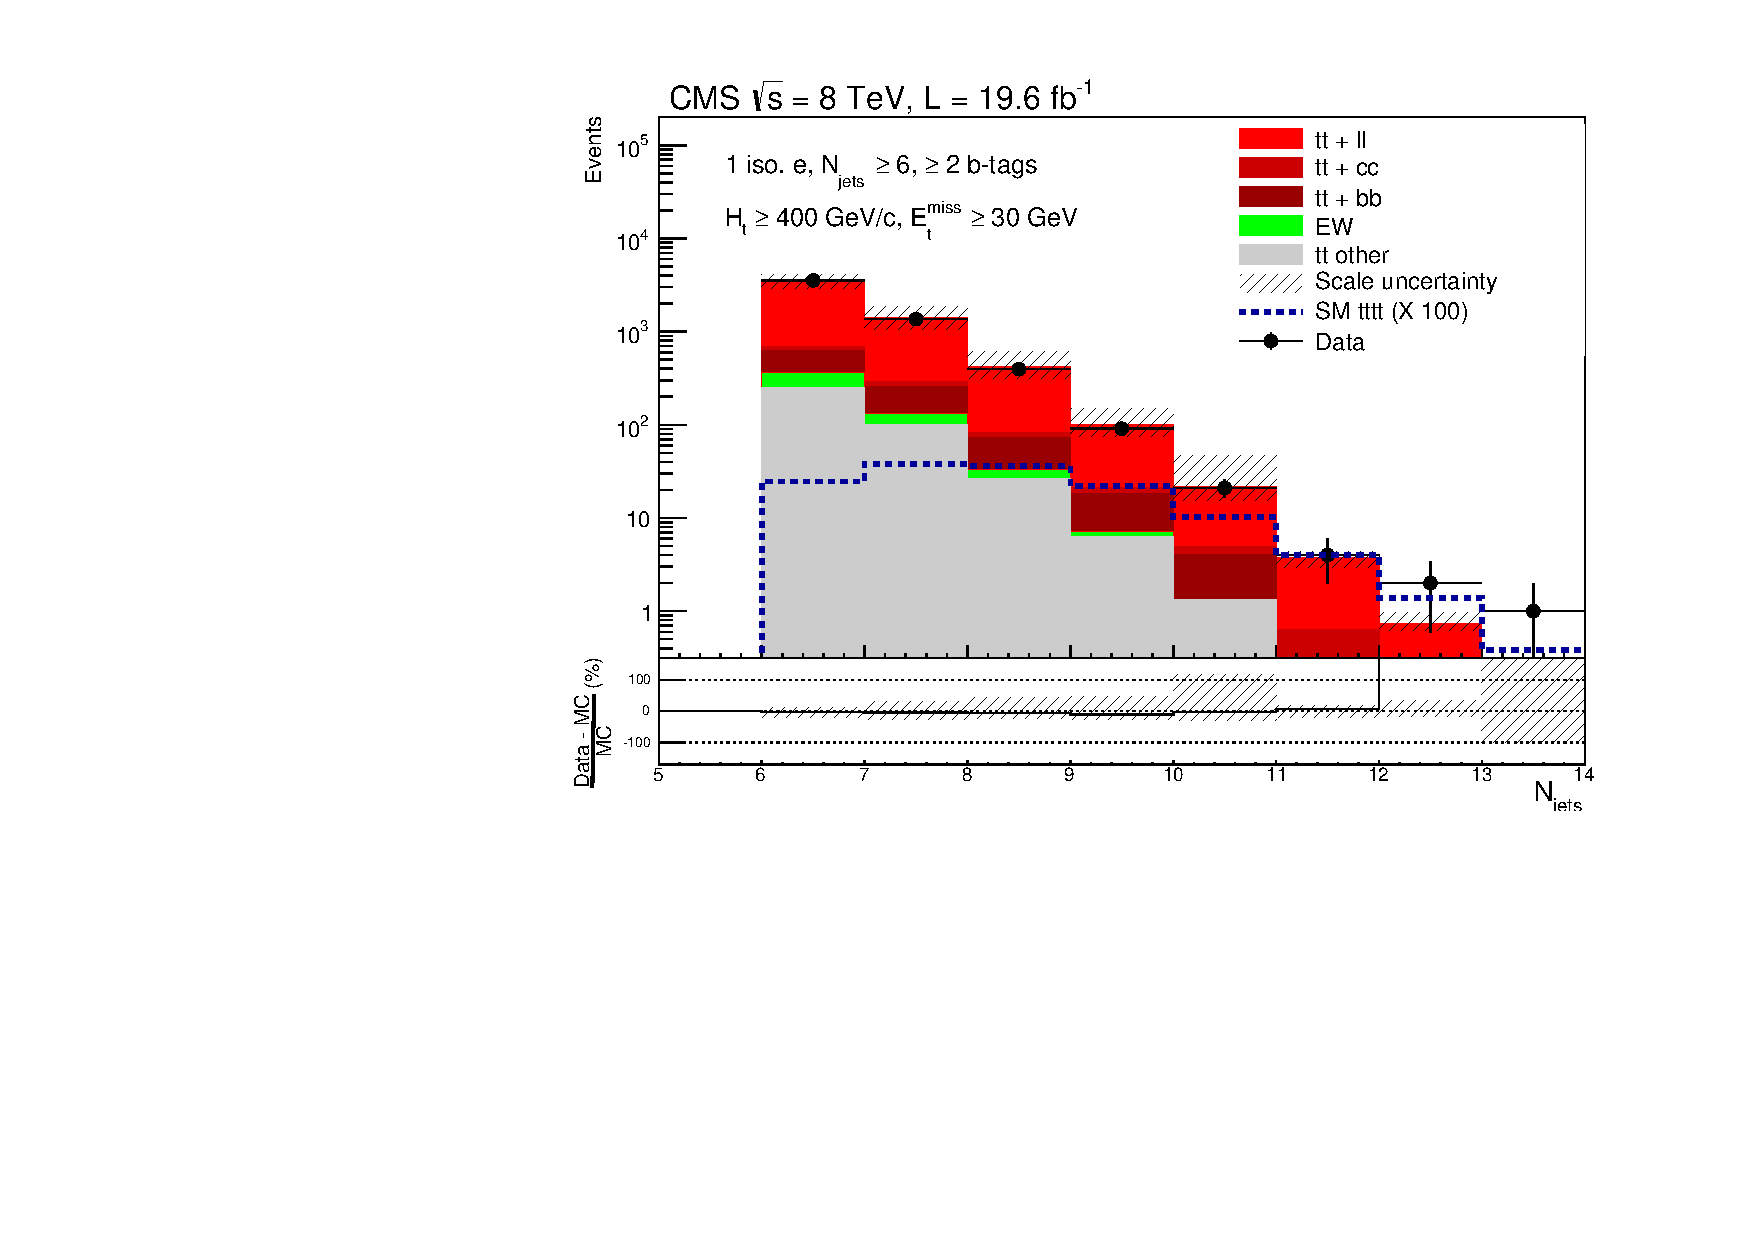
\includegraphics[width=0.49\textwidth]{images/Run1/NbOfSelectedJets_e.pdf}       
    \caption{Data-simulation comparison for \njets for $\mu$ + jets (right) and e + jets (left).}
    \label{fig:datasimnjets}
\end{figure}

\begin{figure}[ht!]
\centering
    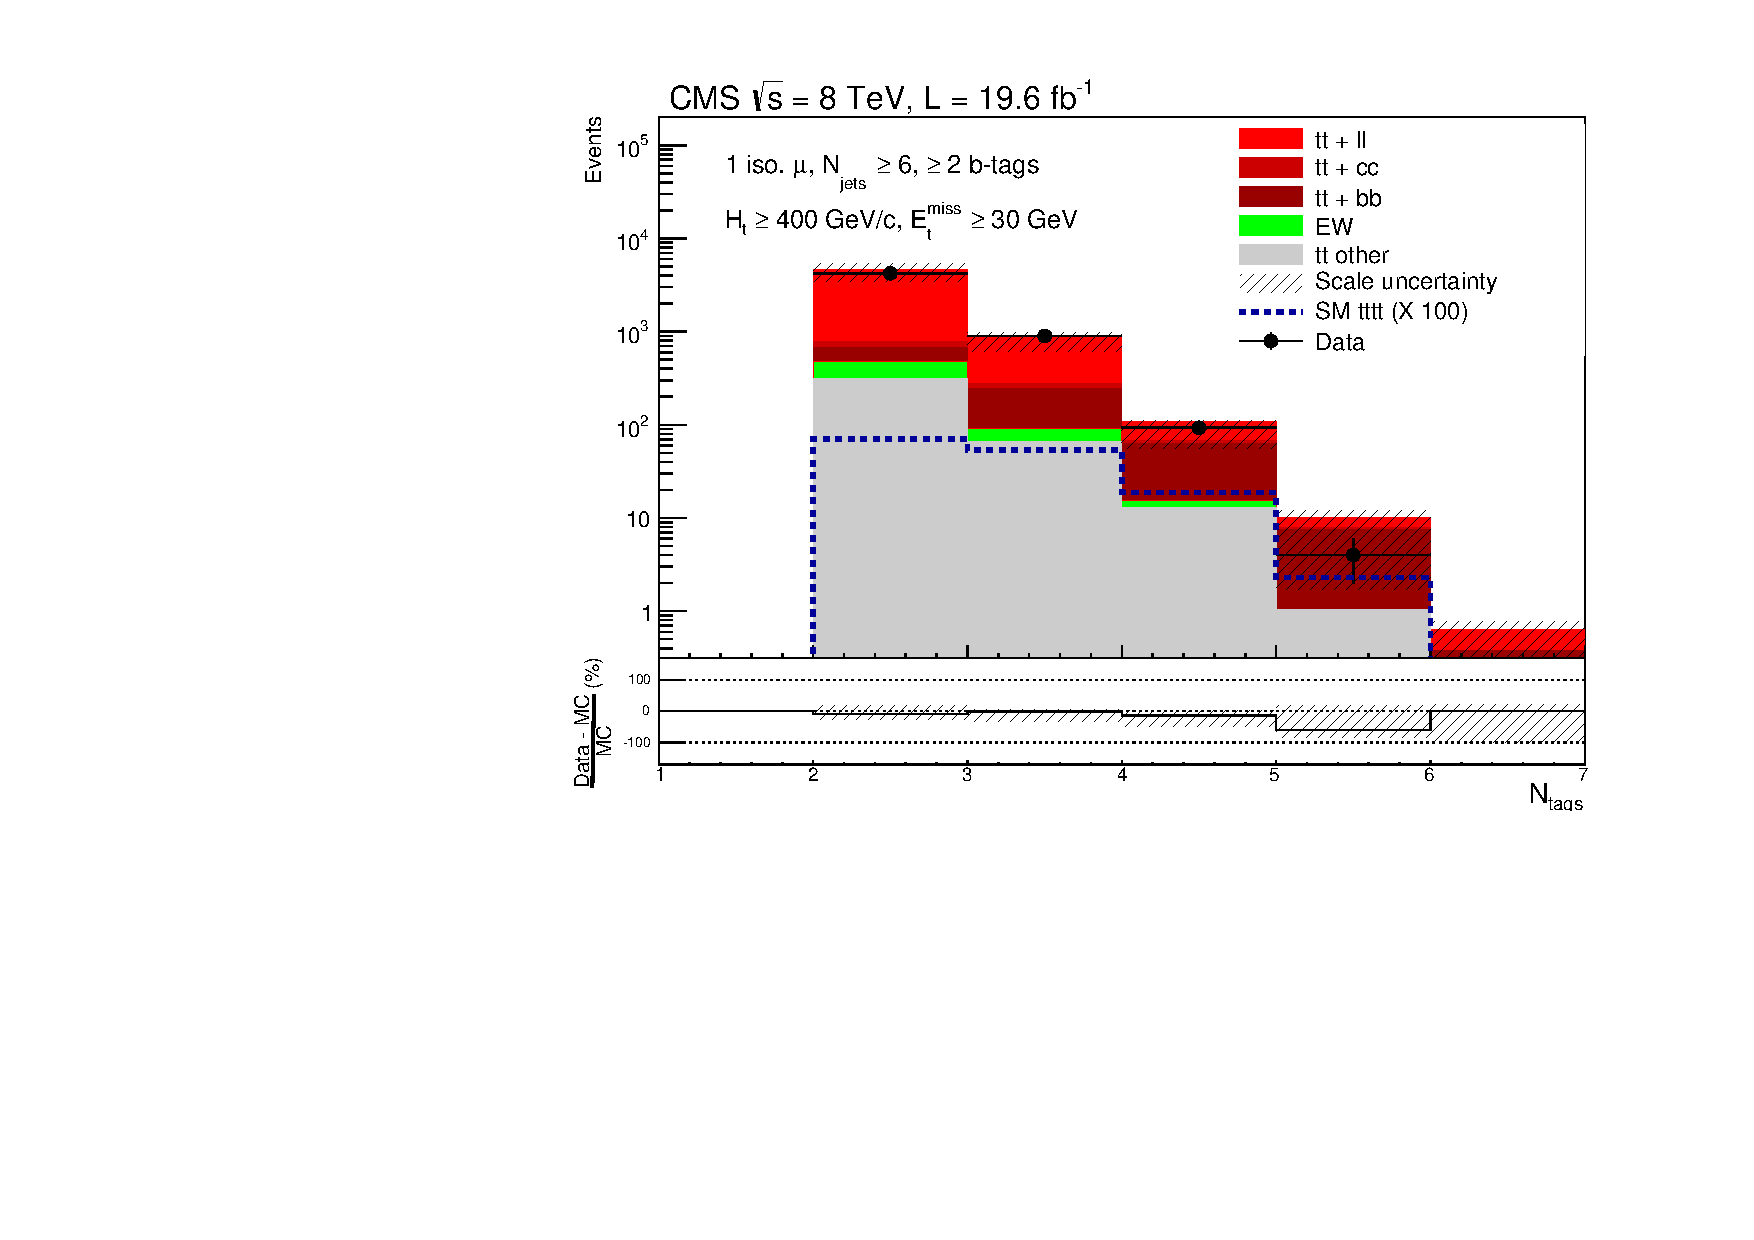
\includegraphics[width=0.49\textwidth]{images/Run1/NbOfSelectedBJets_mu.pdf}
     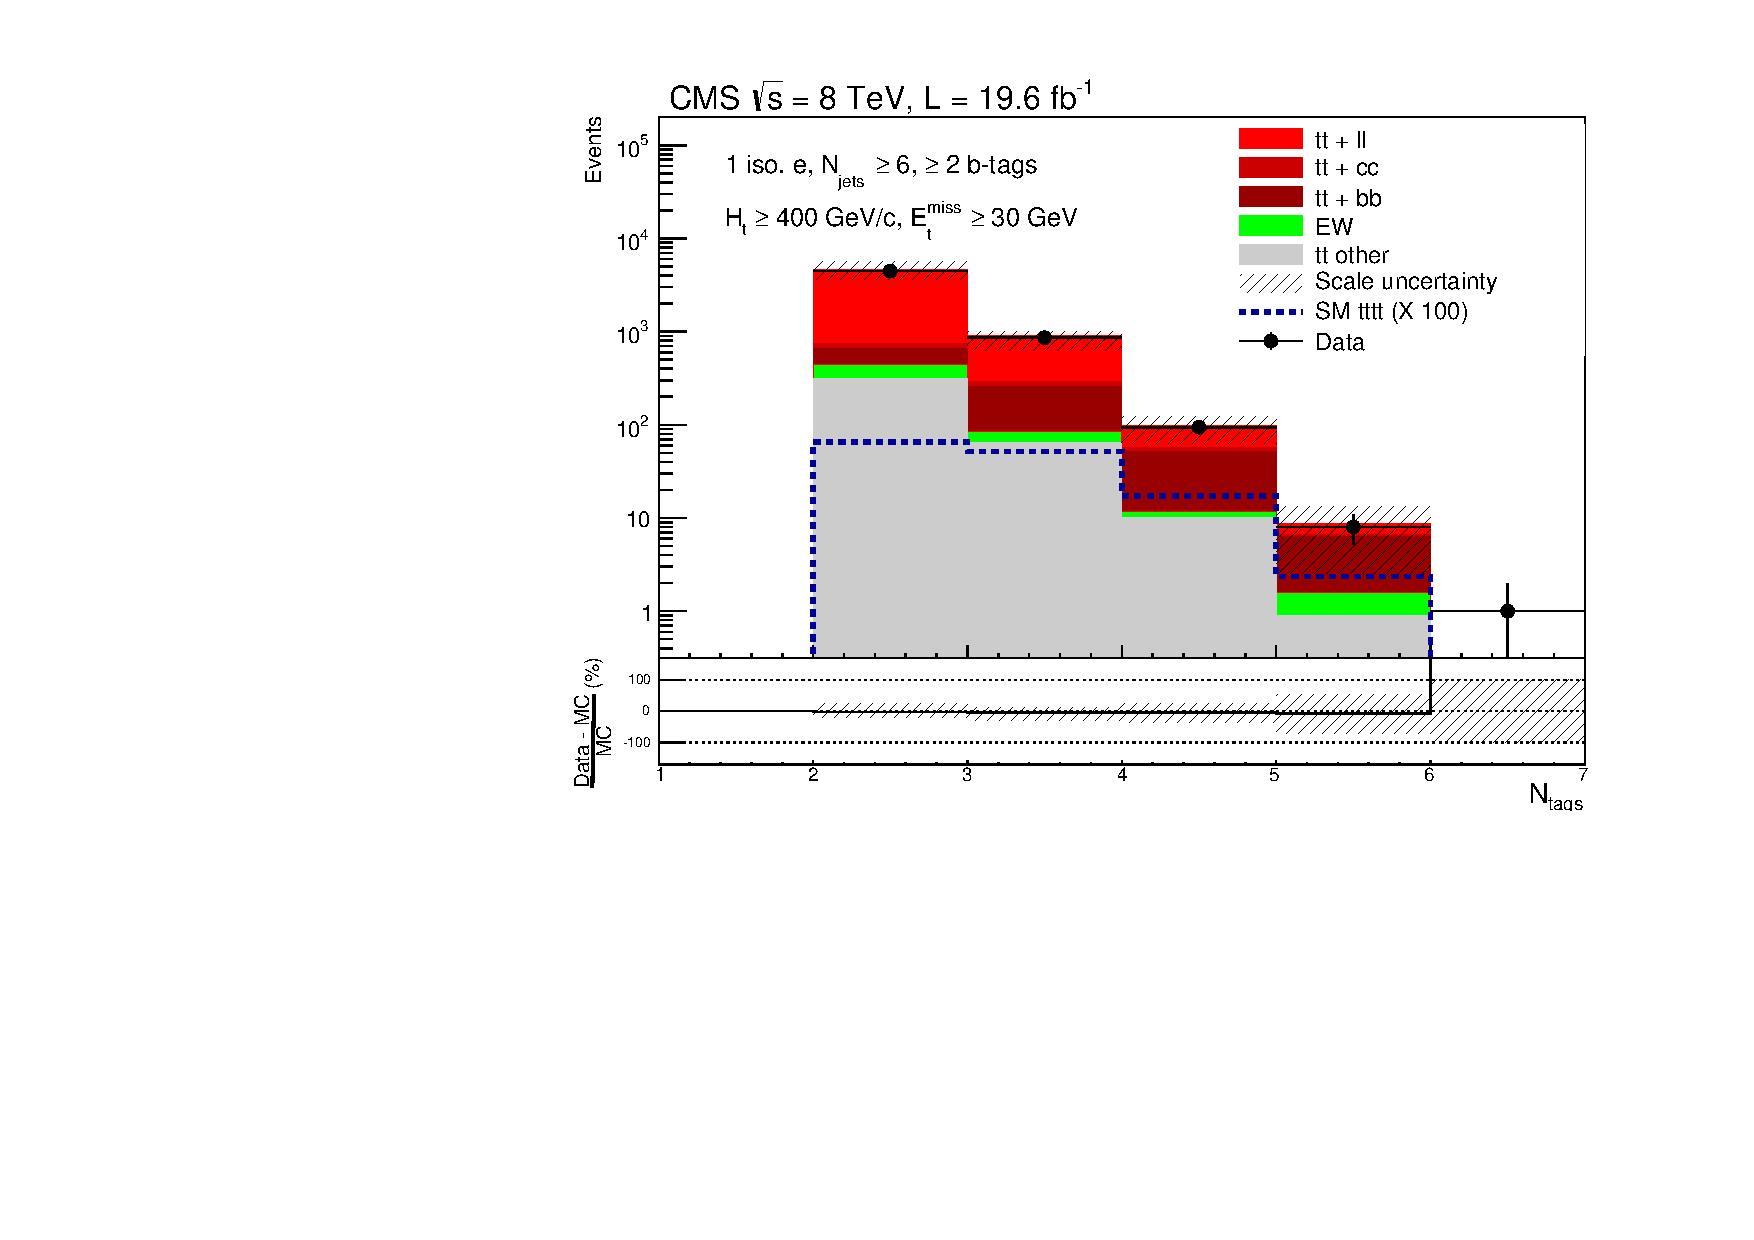
\includegraphics[width=0.49\textwidth]{images/Run1/NbOfSelectedBJets_e.pdf}        
    \caption{Data-simulation comparison for \nbtags for $\mu$ + jets (right) and e + jets (left).}
    \label{fig:datasimnbtags}
\end{figure}

\begin{figure}[ht!]
\centering
    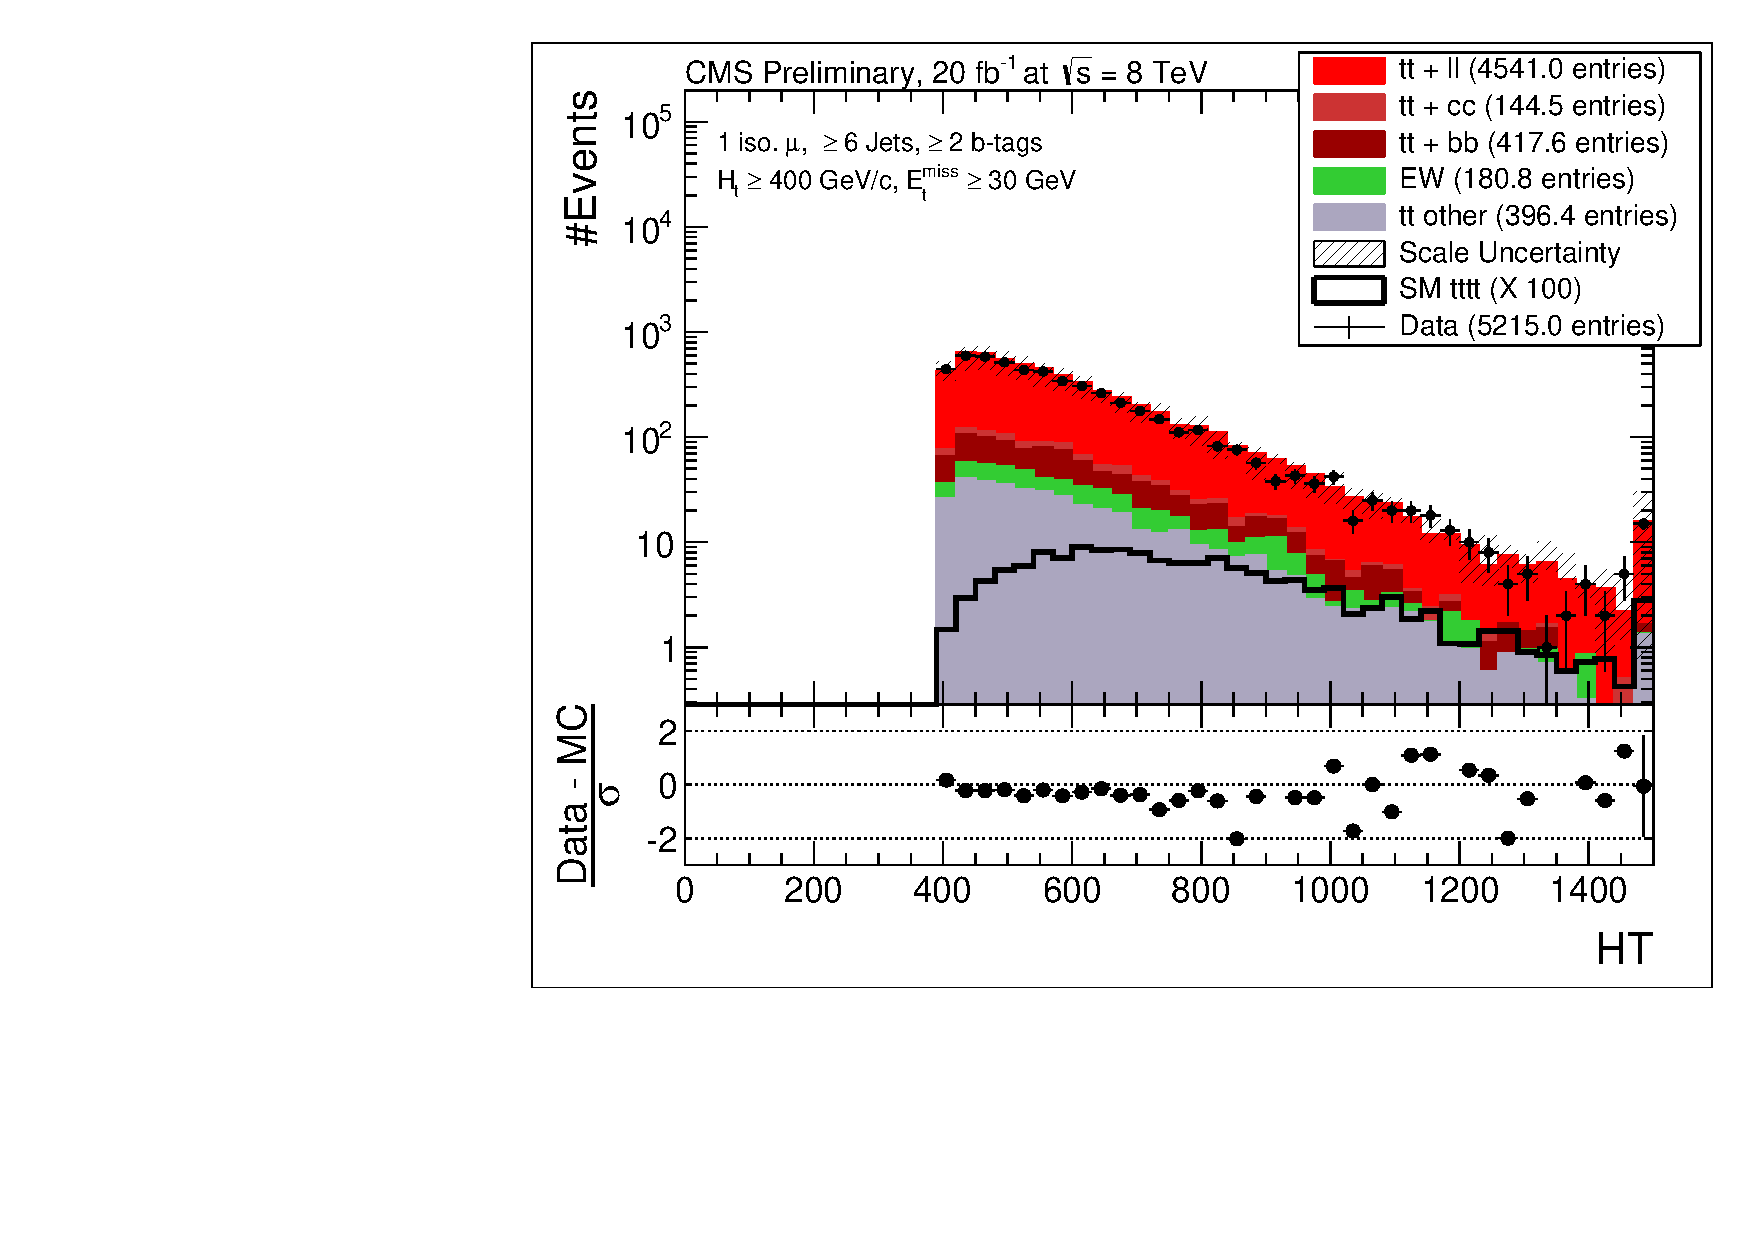
\includegraphics[width=0.49\textwidth]{images/Run1/HT_SelectedJets_StackLogY_Mu.pdf}
     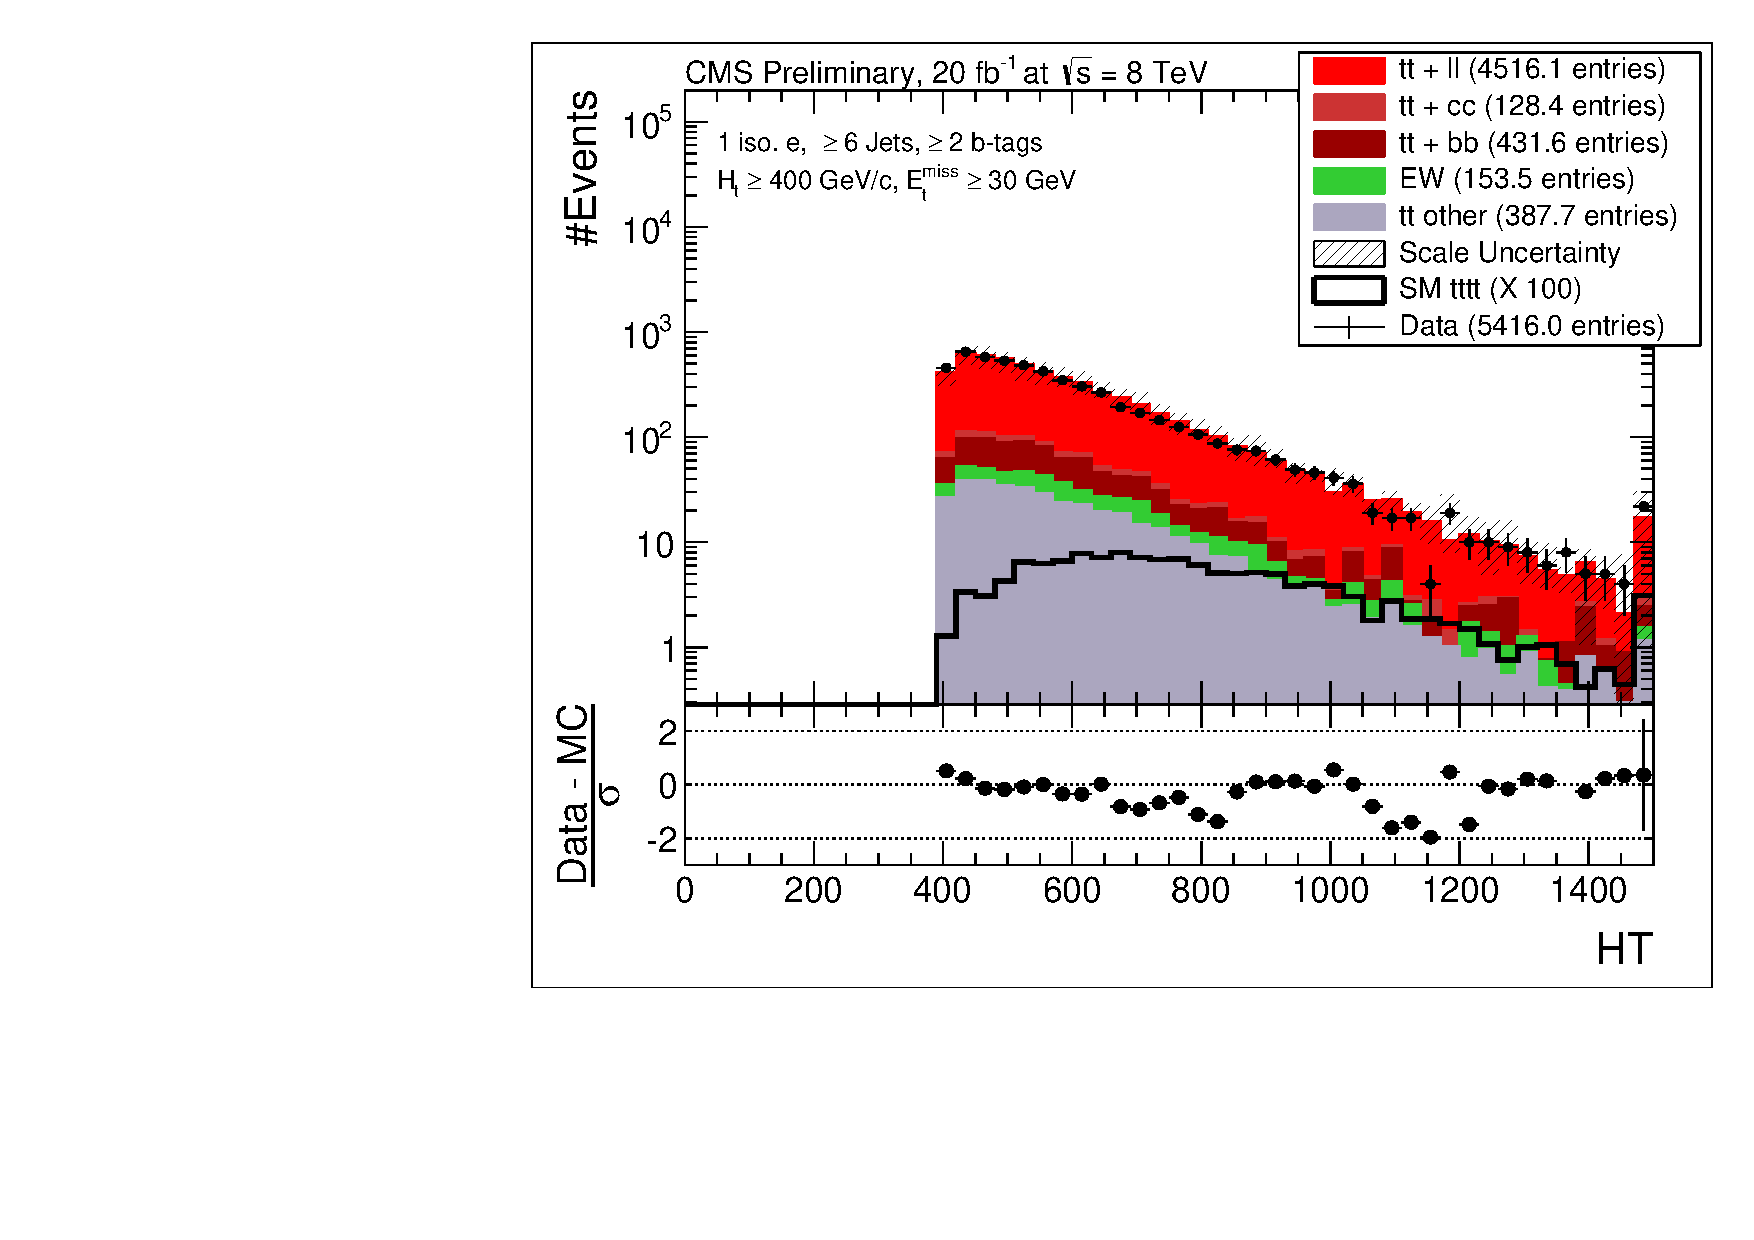
\includegraphics[width=0.49\textwidth]{images/Run1/HT_SelectedJets_StackLogY_e.pdf}          
    \caption{Data-simulation comparison for \HT for $\mu$ + jets (right) and e + jets (left). }
    \label{fig:datasimHT}
\end{figure}

\begin{figure}[ht!]
\centering
    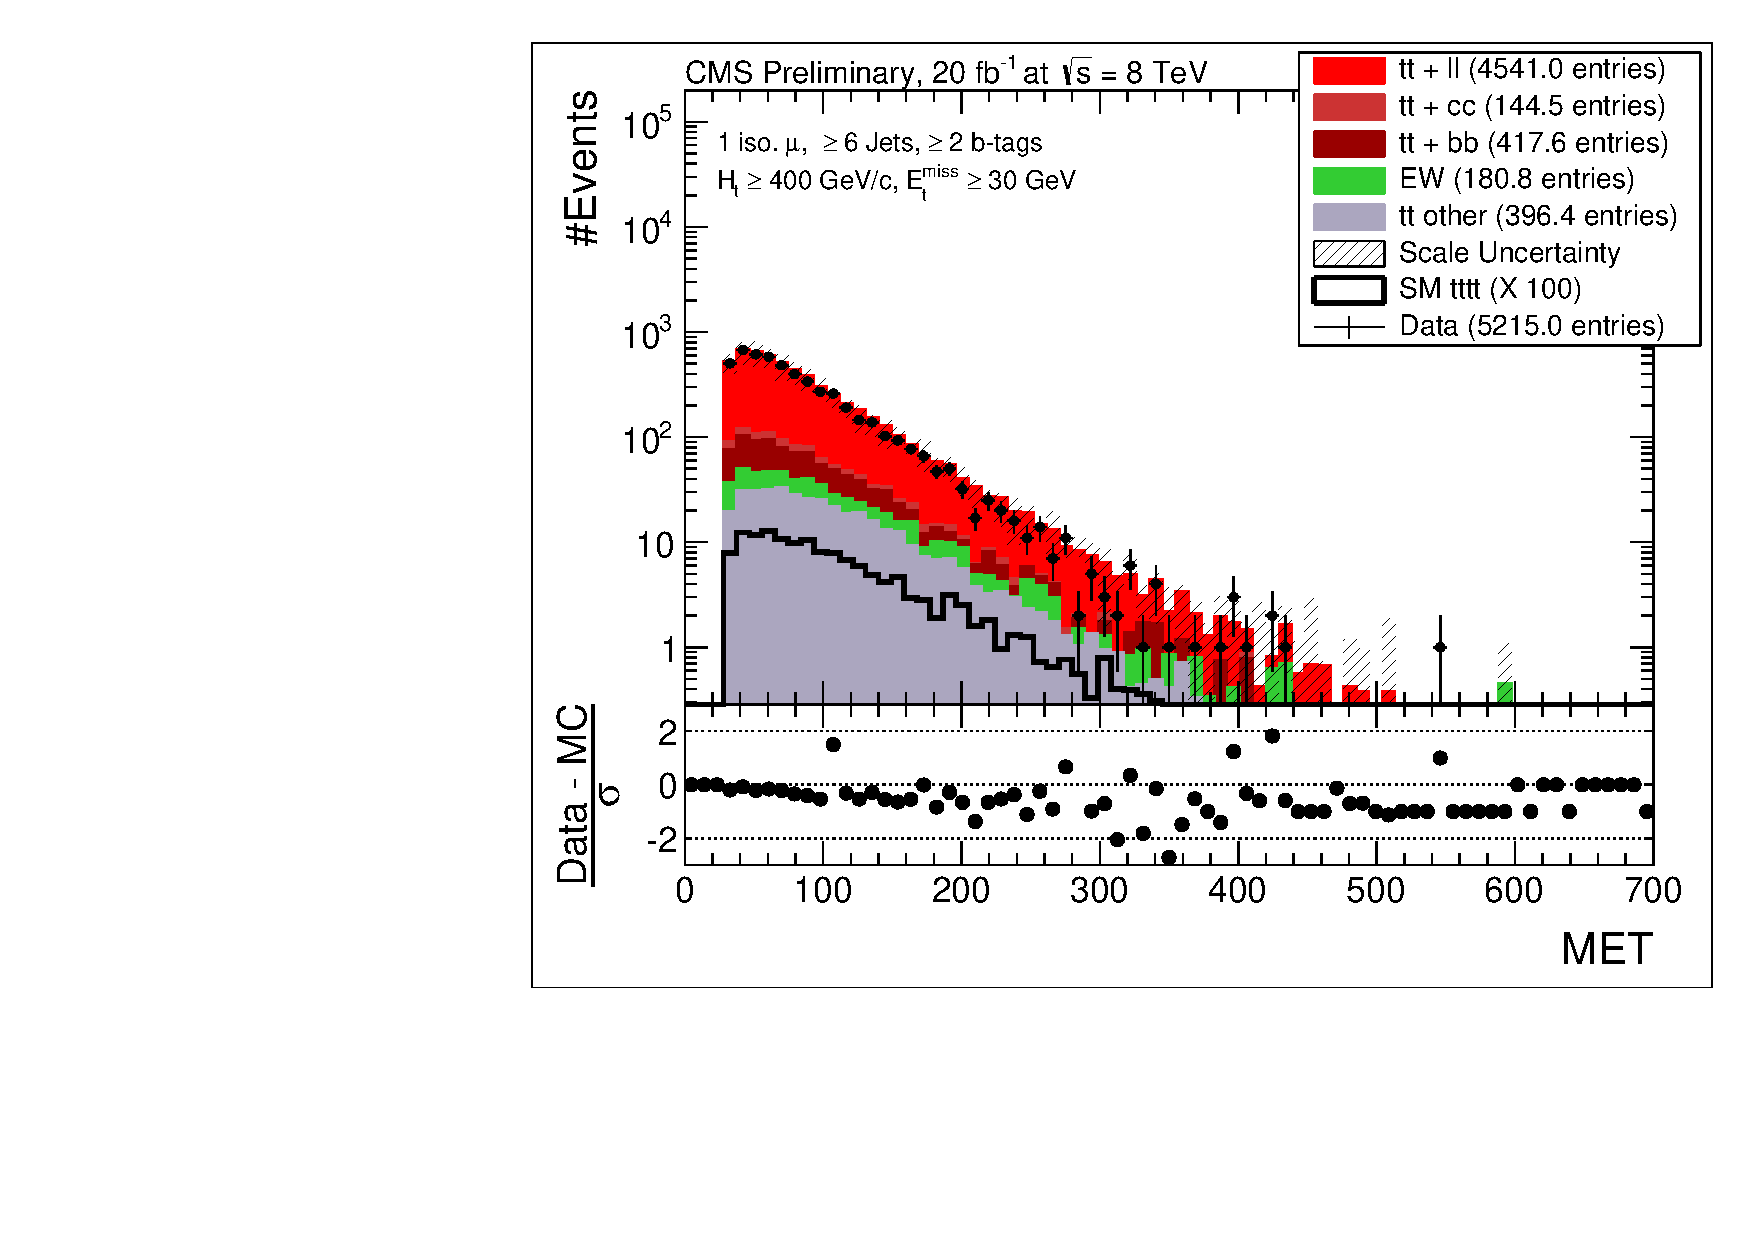
\includegraphics[width=0.49\textwidth]{images/Run1/MET_StackLogY_Mu.pdf}
     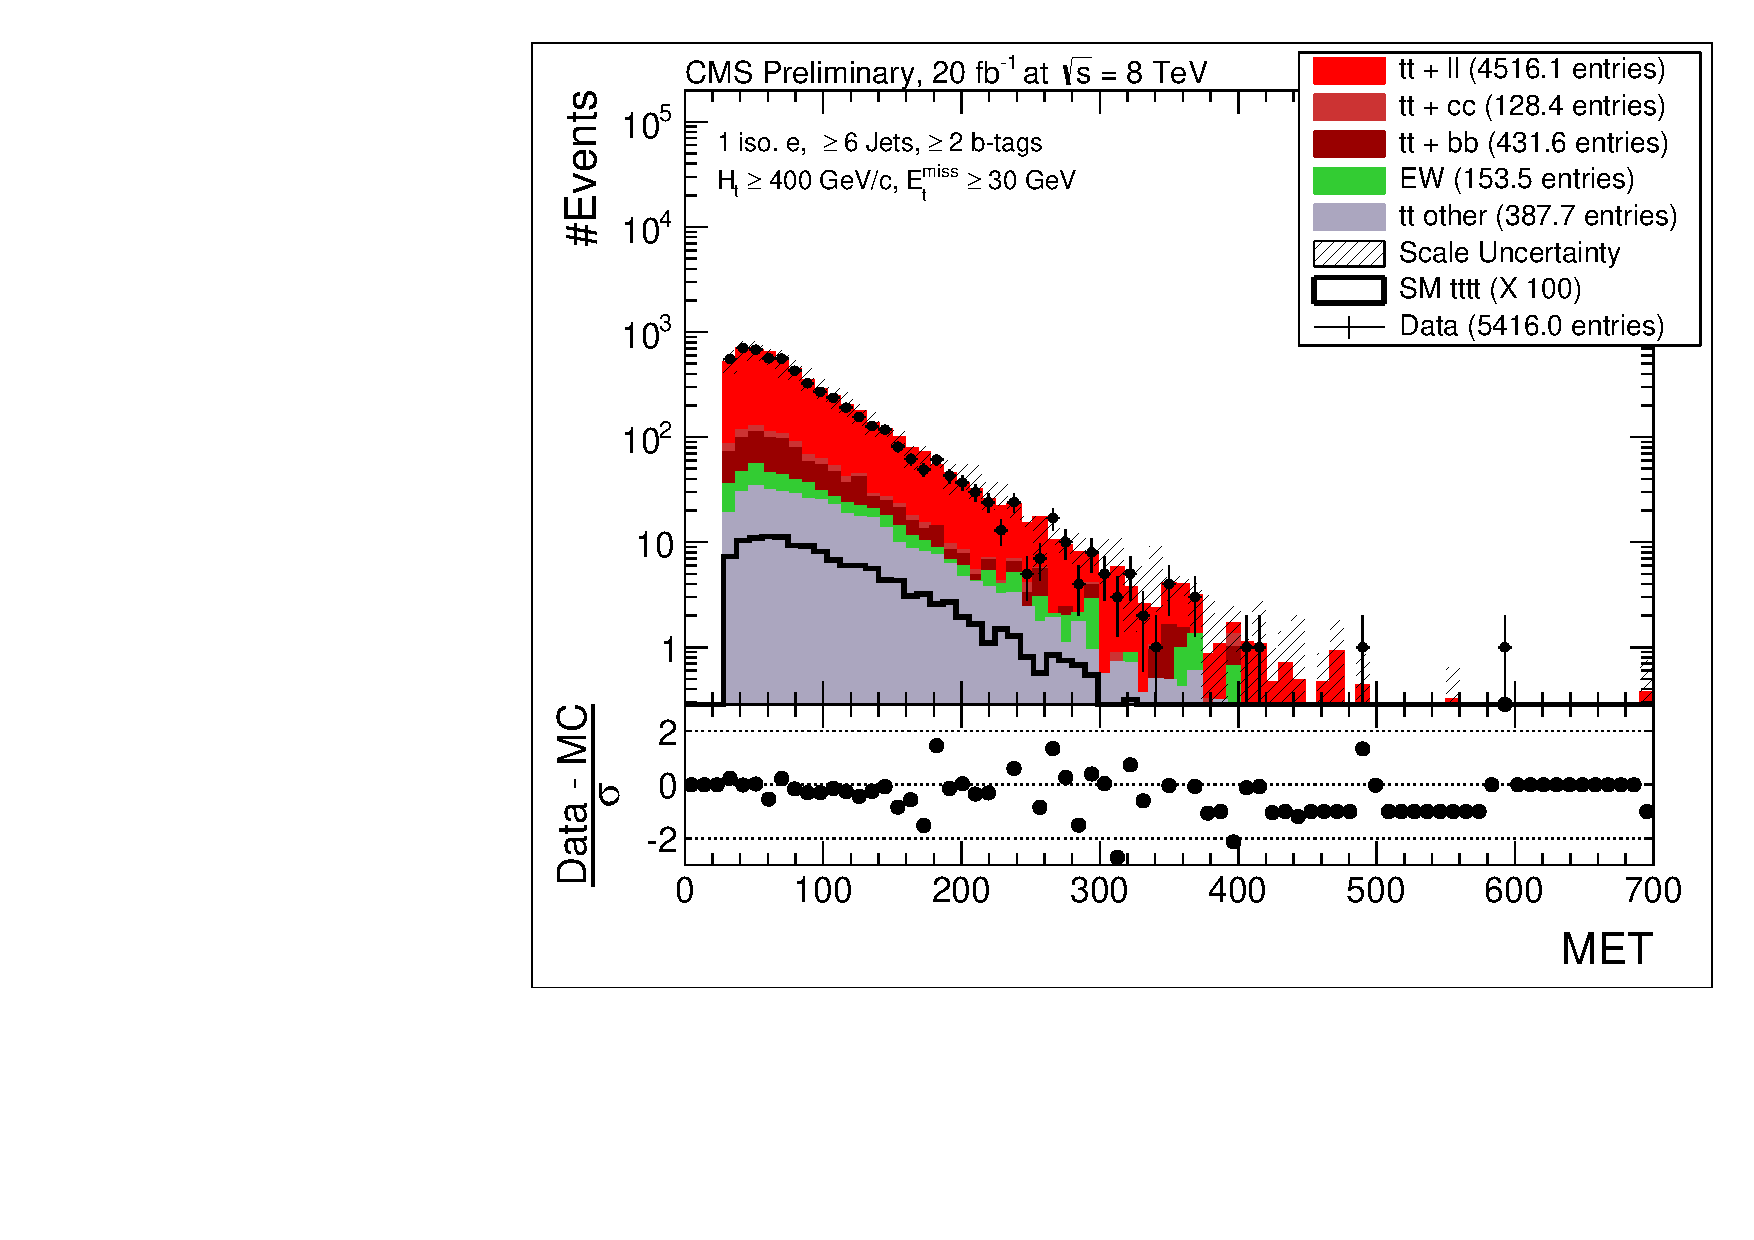
\includegraphics[width=0.49\textwidth]{images/Run1/MET_StackLogY_e.pdf}          
    \caption{Data-simulation comparison for \MET for $\mu$ + jets (right) and e + jets (left). }
    \label{fig:datasimMET}
\end{figure}



\section{Multi-jet background estimation}
\label{sec:QCDbackground}
The presence of multi-jet events within the signal region defined by the baseline selection is investigated in this section. 
%It is rare for multi-jet events to have a highly energetic undetectable particle. Therefore, the $\MET$ distributions for multi-jet events typically peak at \fxnote*{more specific?}{low values}. 
It can be seen from the MET distributions in Fig.~\ref{fig:datasimMET} that the data agrees well with the simulation at low values which suggests there are very few multi-jet events which pass the tight requirements in the baseline selection. 
%Due to this small number of events, it is not possible to use multi-jet MC to estimate this background. In this case, a data-driven method known as the \fxnote*{ref?}{ABCD method} may be used. This method proceeds by selecting two uncorrelated variables from the object or baseline selection and defining three control regions (A,B,C) and one signal region (D) in the 2-dimensional phase space of these variables. The event variable \MET and the lepton variable RelIso were selected as they are \fxnote*{uncorrelated proof??}{uncorrelated} and 
The defined regions in the uncorrelated variables of \MET and $RelIso$ are shown below. The upper bound in $RelIso$ is restricted by the minimum $RelIso$ values required by the HLT in the single muon and single electron streams.\\

For the muon channel these are:
\begin{itemize}
\setlength\itemsep{0em}
\item A : 30 $<\MET<$ 500, 0.1 $<$ RelIso $<$ 0.15
\item B : 0 $<\MET<$ 30, 0.1 $<$ RelIso $<$ 0.15
\item C : 0 $<\MET<$ 30, 0 $<$ RelIso $<$ 0.1
\item D : 30 $<\MET<$ 500, 0 $<$ RelIso $<$ 0.1
\end{itemize}
For the \eplusjets:
\begin{itemize}
\itemsep0em
\item A : 30 $<\MET<$ 500, 0.12 $<$ RelIso $<$ 0.2
\item B : 0 $<\MET<$ 30, 0.12 $<$ RelIso $<$ 0.2
\item C : 0 $<\MET<$ 30, 0 $<$ RelIso $<$ 0.12
\item D : 30 $<\MET<$ 500, 0 $<$ RelIso $<$ 0.12
\end{itemize}

%It is assumed that the multi-jet background can be estimated from the data minus the background expectation from all of the other MC samples considered in Section~\ref{sec:datasimulation}. 
The results of the background subtraction from data and the defined ABCD regions are shown in Fig.~\ref{fig:QCDplots}.
The number of multi-jet events, N$_{\textrm{multi-jet}}$, in each of the control regions are used to predict the number of multi-jet events in region D using Eq.~\ref{N-multi-jet}, the results of which are shown in Table~\ref{tab:multijet}.

\begin{figure}[!ht]
    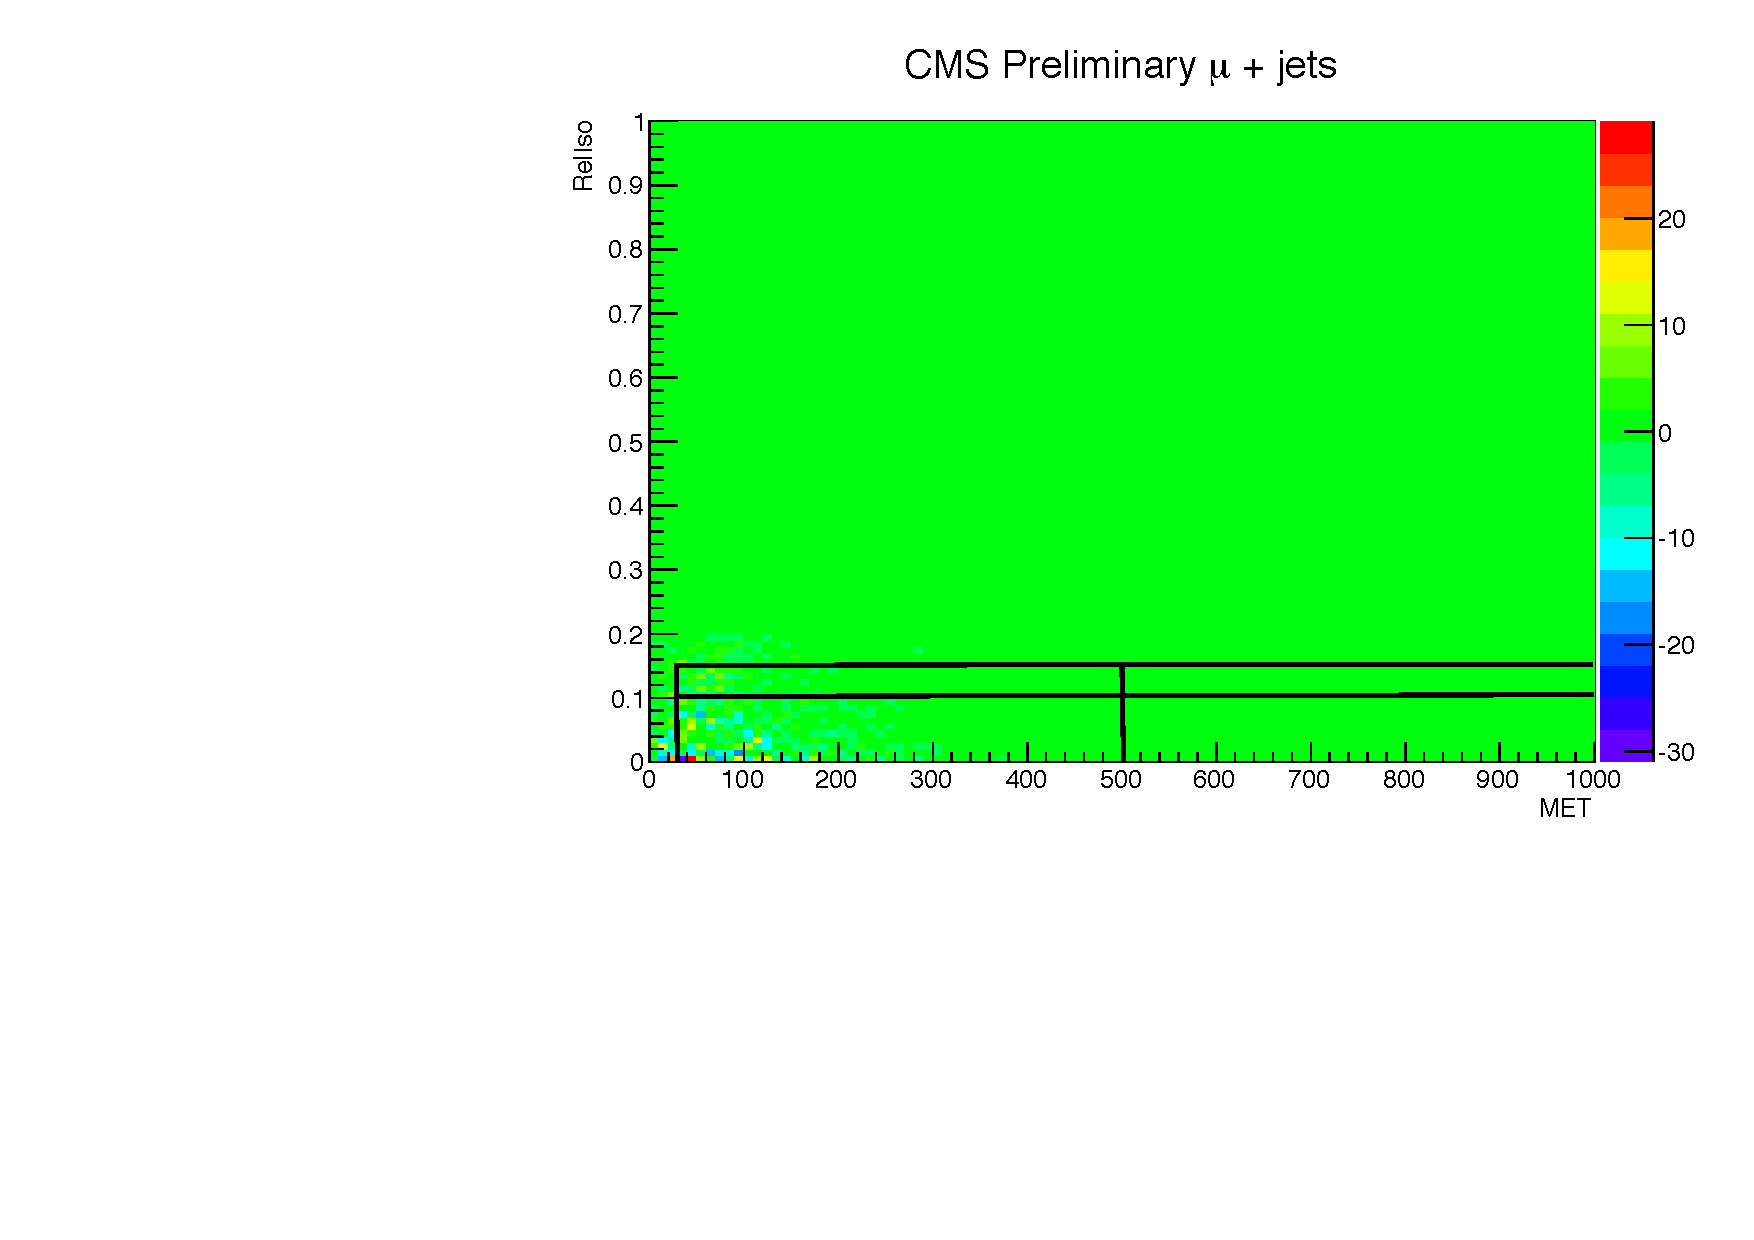
\includegraphics[width=0.49\textwidth]{images/Run1/Data_Minus_MC_Mu-1.pdf}
    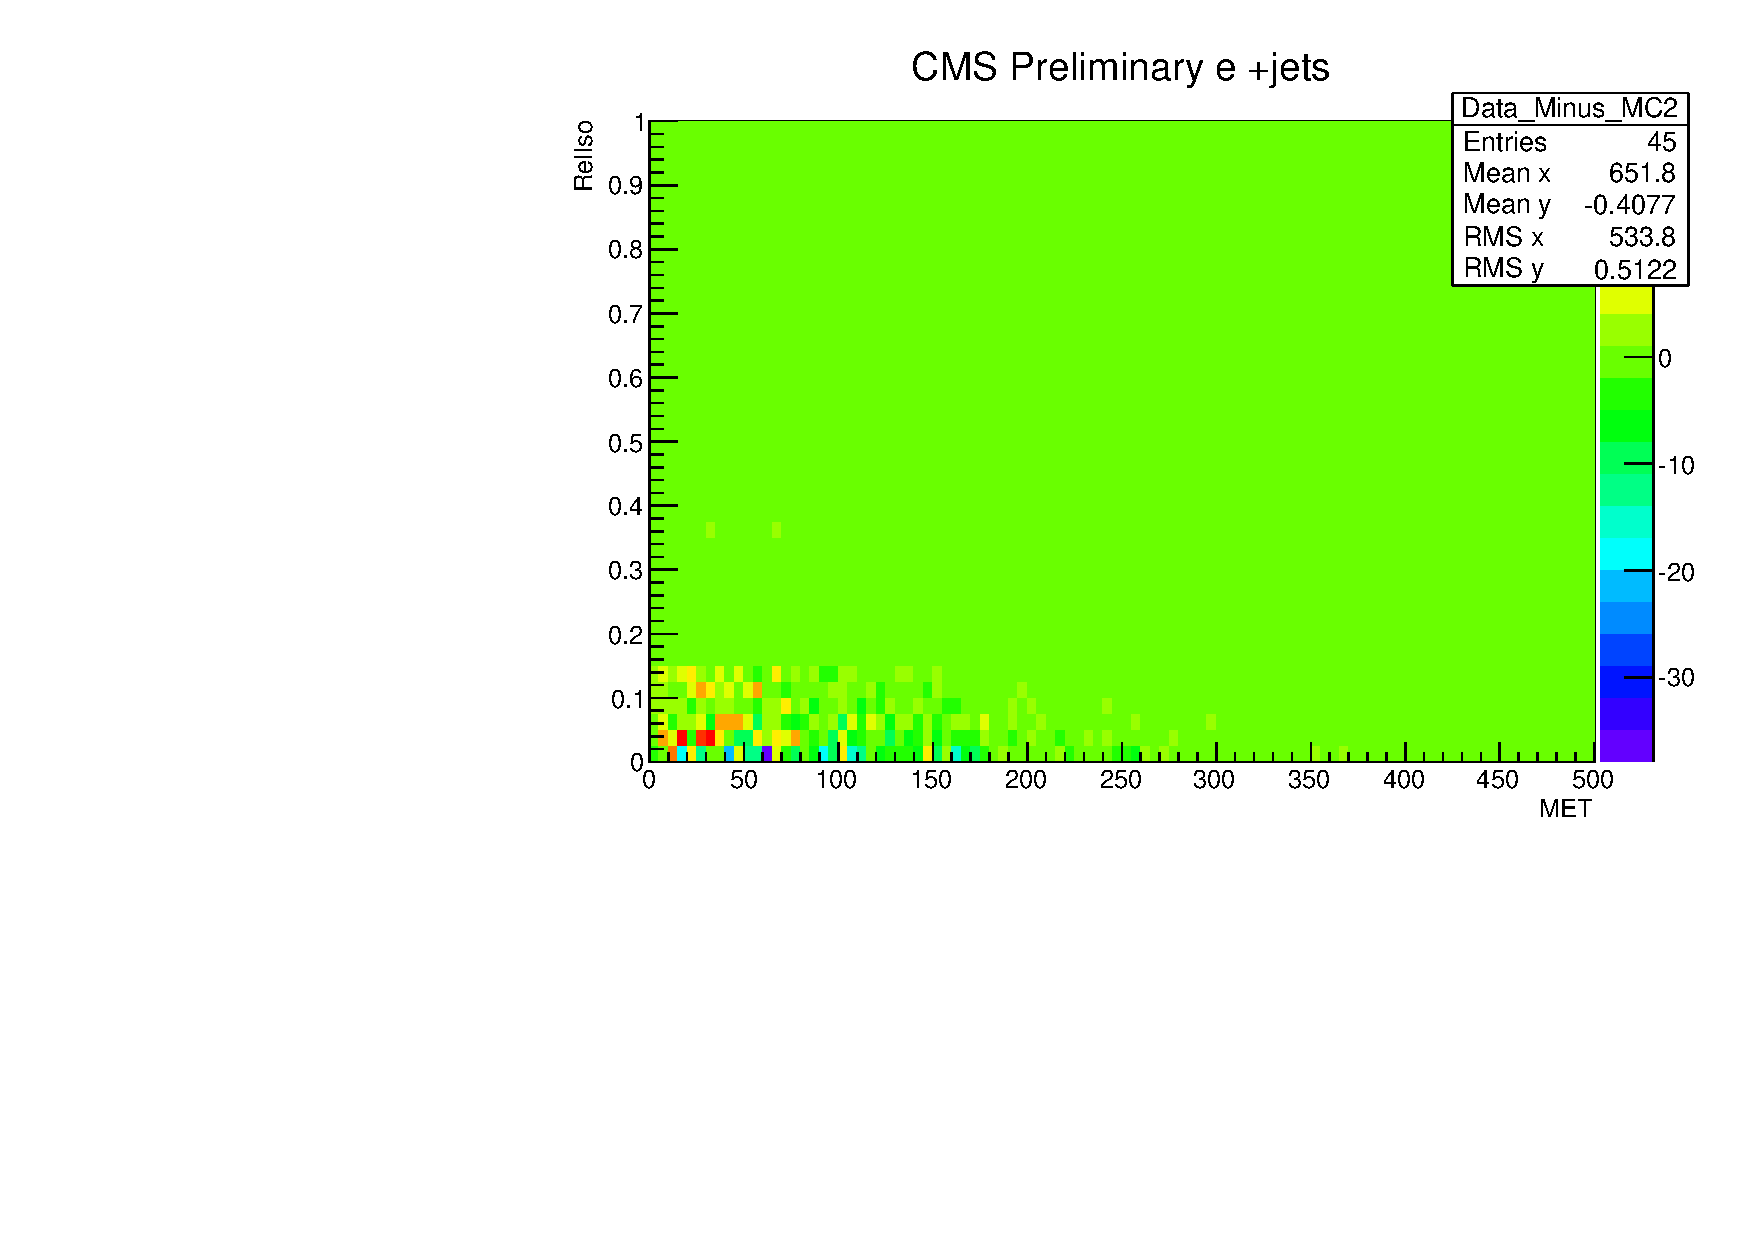
\includegraphics[width=0.49\textwidth]{images/Run1/Data_Minus_MC_El.pdf}
    \caption{Data minus MC background for MET vs lepton iso for $\mu$ + jets (right) and e + jets (left).}
    \label{fig:QCDplots}
\end{figure}


\begin{equation}
\frac{\textrm{N}^{\textrm{B}}_{\textrm{multi-jet}}}{\textrm{N}^{\textrm{A}}_{\textrm{multi-jet}}} = \frac{\textrm{N}^{\textrm{C}}_{\textrm{multi-jet}}}{\textrm{N}^{\textrm{D}}_{\textrm{multi-jet}}}
\label{N-multi-jet}
\end{equation}

\begin{table}[ht!]
\caption{Multi-jet estimation}
\centering
\begin{tabular}{|c |c |c |c |c |}
 \hline 
 Channel & N$^{\textrm{A}}_{\textrm{multi-jet}}$  & N$^{\textrm{B}}_{\textrm{multi-jet}}$ & N$^{\textrm{C}}_{\textrm{multi-jet}}$ & Prediction for N$^{\textrm{D}}_{\textrm{multi-jet}}$  \\
  \hline
$\mu$ + jets & 19.1 & 16.1 & -16.8 & -20  \\
 \hline
$e$ + jets & 36.8  & 50.8 & 62.7 &45.5  \\
\hline
\end{tabular}
\label{tab:multijet}
\end{table}

As the the number of \ttbar events in simulation has fluctuated to be greater than the data in region C in the muon channel, the prediction for the signal region D is negative. As this prediction is unphysical, the number of events is estimated to be zero in the muon channel. In the electron, 45.5 multi-jet events are predicted which is considered negligible at $<1\%$ of the massive \ttbar background. Hence, the multi-jet background is not considered further.
\fxnote{scale up scale down...200\% uncertainty?}

\section{Discriminating between signal and background}
\label{sec:discriminating}
The dominant background process after the baseline selection is \ttbar production. It is three orders of magnitude greater than the \tttt signal process in the signal region. This motivates the search for variables which can discriminate between these two processes. There are three main features which can be used to discriminate; the number of top quarks which can be reconstructed in the event, the number of b-jets found in each event, and event activity such as \HT.

\subsection{Top quark content}
\label{sec:topContent}
In the single lepton channel for \tttt production, there are three top quarks where the W boson decays hadronically, these will be referred to as hadronic top quarks. For the main background of \ttbar there is only one hadronic top quark. Additional jets in \ttbar come from \fxnote*{assume previously defined}{ISR or FSR} in order to satisfy the requirements of the baseline selection. Therefore, it should only be possible to reconstruct more than one top quark from three jets originating from it's hadronic decay in \tttt but not in \ttbar. However, the \antikt algorithm can only distinguish separate jets if they have \DR$>0.5$ between them, hence it may not always be possible to reconstruct all hadronic top quarks. To ascertain whether this might be a powerful technique for separating \tttt and \ttbar or not, 1000 \tttt and 1000 \ttbar events were analysed where there was one muon with \PT $>$ 26 GeV and exactly 6 jets with \PT $>$ 30 and $\lvert \eta \rvert<$ 2.5. Hadronic top quarks are considered reconstructible at parton level if they decayed into jets with \DR  $>$  0.5. The number of reconstructible hadronic top quarks for \tttt and \ttbar are shown in Fig.~\ref{fig:ReconHadTops}.

\begin{figure}[!ht]
    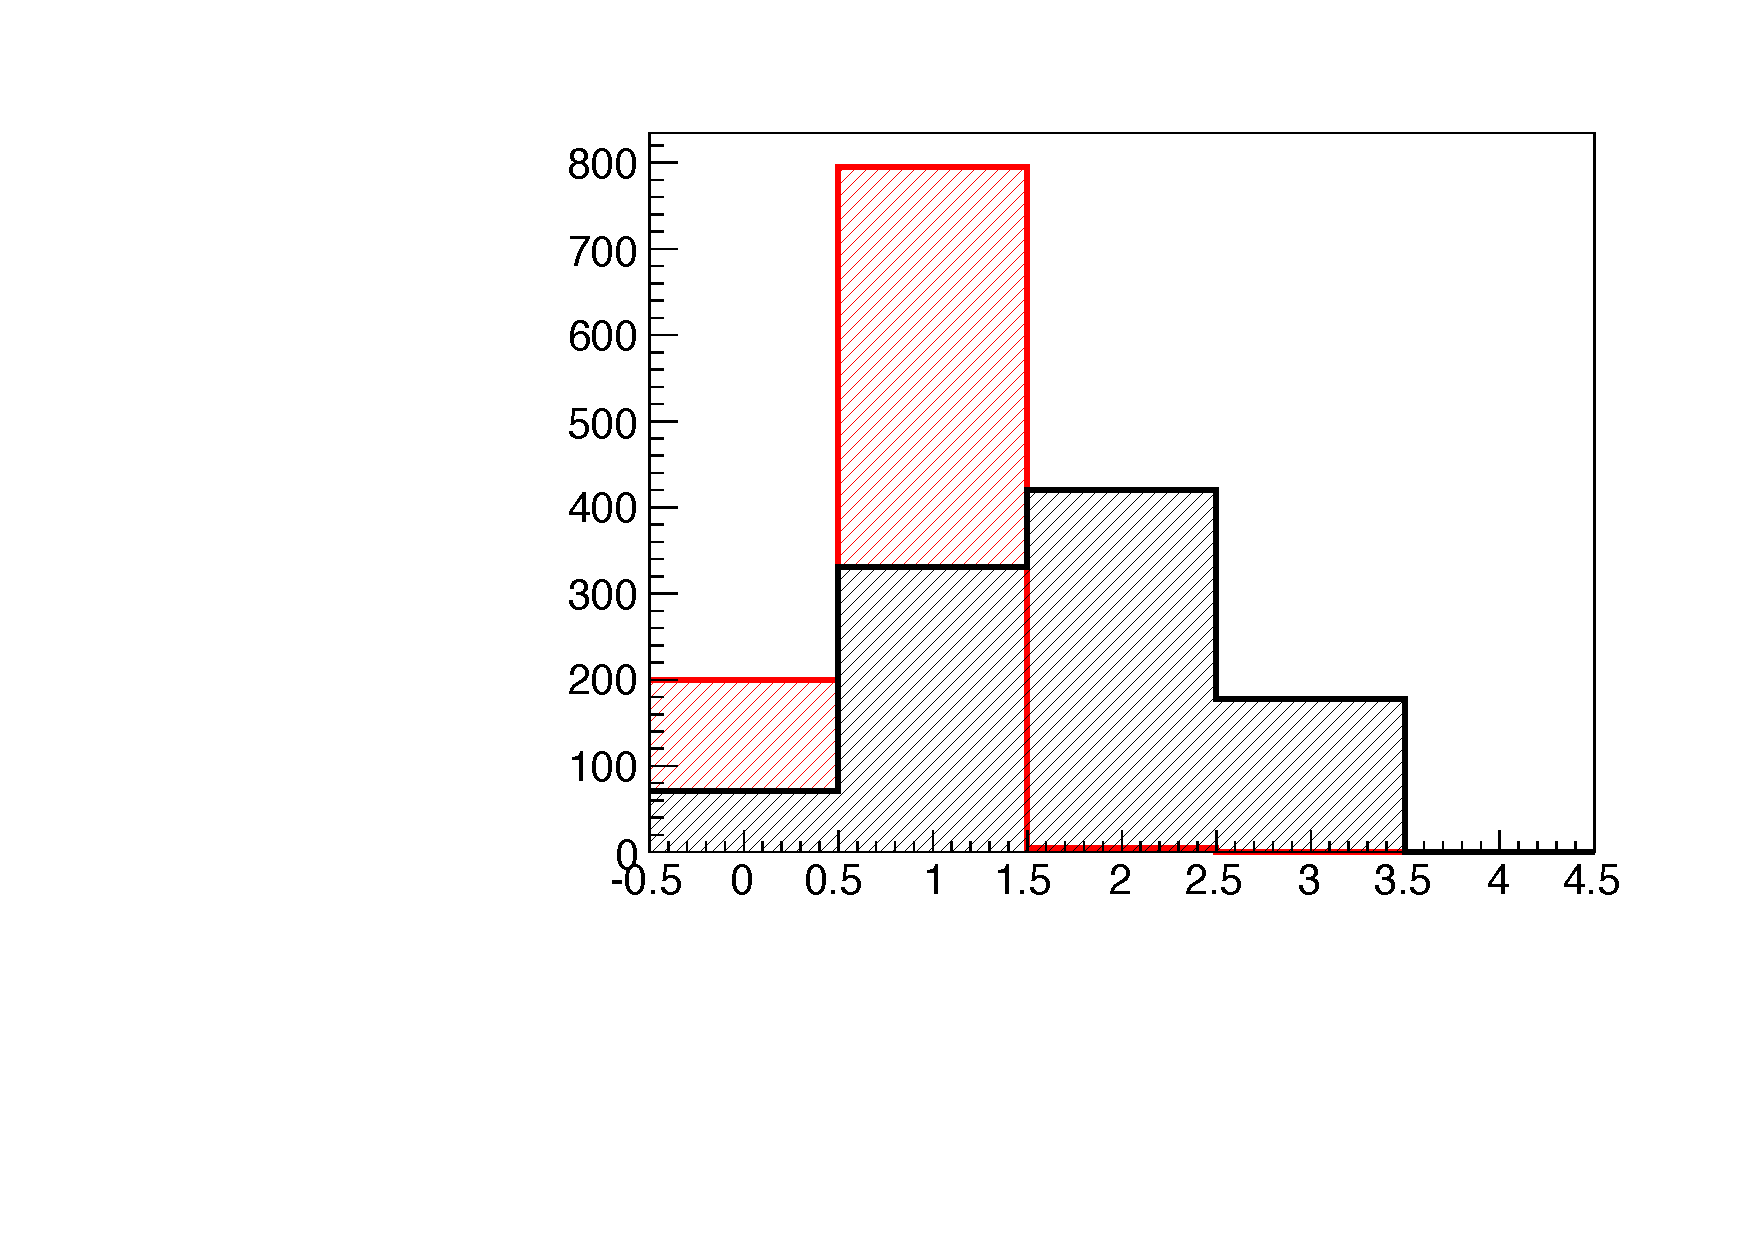
\includegraphics[width=0.6\textwidth]{images/Run1/ReconstructibleTops.pdf}
    \caption{The number of reconstructible hadronic top quarks in \tttt and \ttbar}
    \label{fig:ReconHadTops}
\end{figure}

For \tttt production at parton level it is possible to reconstruct more than one hadronic top quark $\approx$ 63 $\%$ of the time compared to a negligible number of times in \ttbar, as is evident in the Fig.~\ref{fig:ReconHadTops}. Hence, using the number of hadronic tops can be assumed to be a powerful variable worth investigating. One obstacle to this is the large number of ways in which the jets can be combined in events with \njets $\geq 6$.\fxnote{more on combinatorics? -> but James' work} This motivates the use of multi-variate analysis to distinguish between good tri-jet combinations and bad tri-jet combinations, where a tri-jet refers to any given combination of three jets. Figure~\ref{fig:TopBDTinput} shows the minimal number of discriminating variables which are used including:\\
\textbf{Tri-jet invariant mass} - Good tri-jet combinations should have an invariant mass distribution which peaks around the top mass.\\
\textbf{Di-jet invariant mass} - The di-jet combination is formed from the two jets with the smallest \DR separation. The invariant mass distribution should peak around the W mass.\\
\textbf{\ptrat} - This is the ratio of the vectorial \pt to the scalar sum of the \pt of the jets in the tri-jet combination.\\
\textbf{\DPTW} - This is the \Dphi separation between the tri-jet and di-jet system.\\
\textbf{\DPTb} - This is the \Dphi separation between the tri-jet and remaining jet not included in the di-jet system.\\
\textbf{\CSVj} - For the jet not used in the di-jet system, the CSV b-tagging discriminator value is used.\\

\begin{figure}[ht!]
\centering
    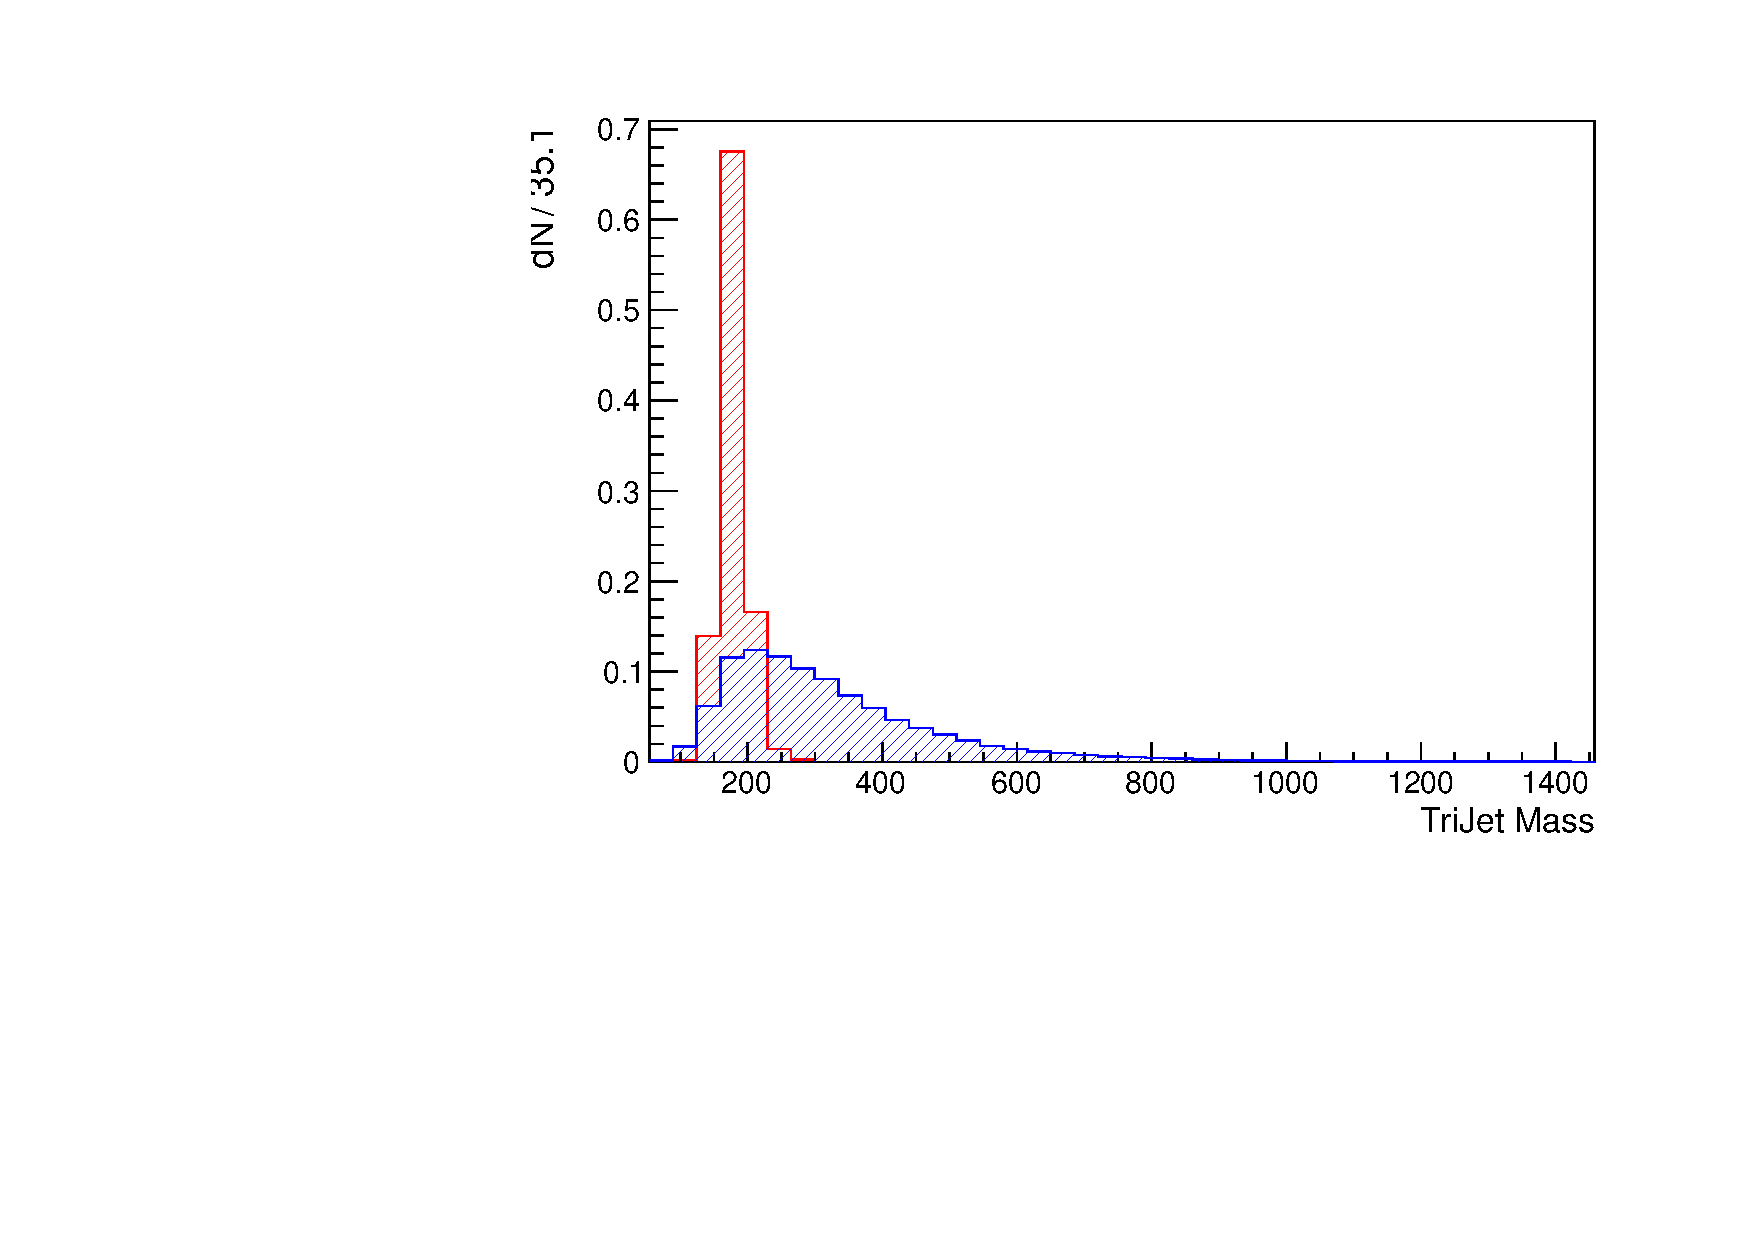
\includegraphics[width=0.49\textwidth]{images/Run1/TriJetMass.pdf}
     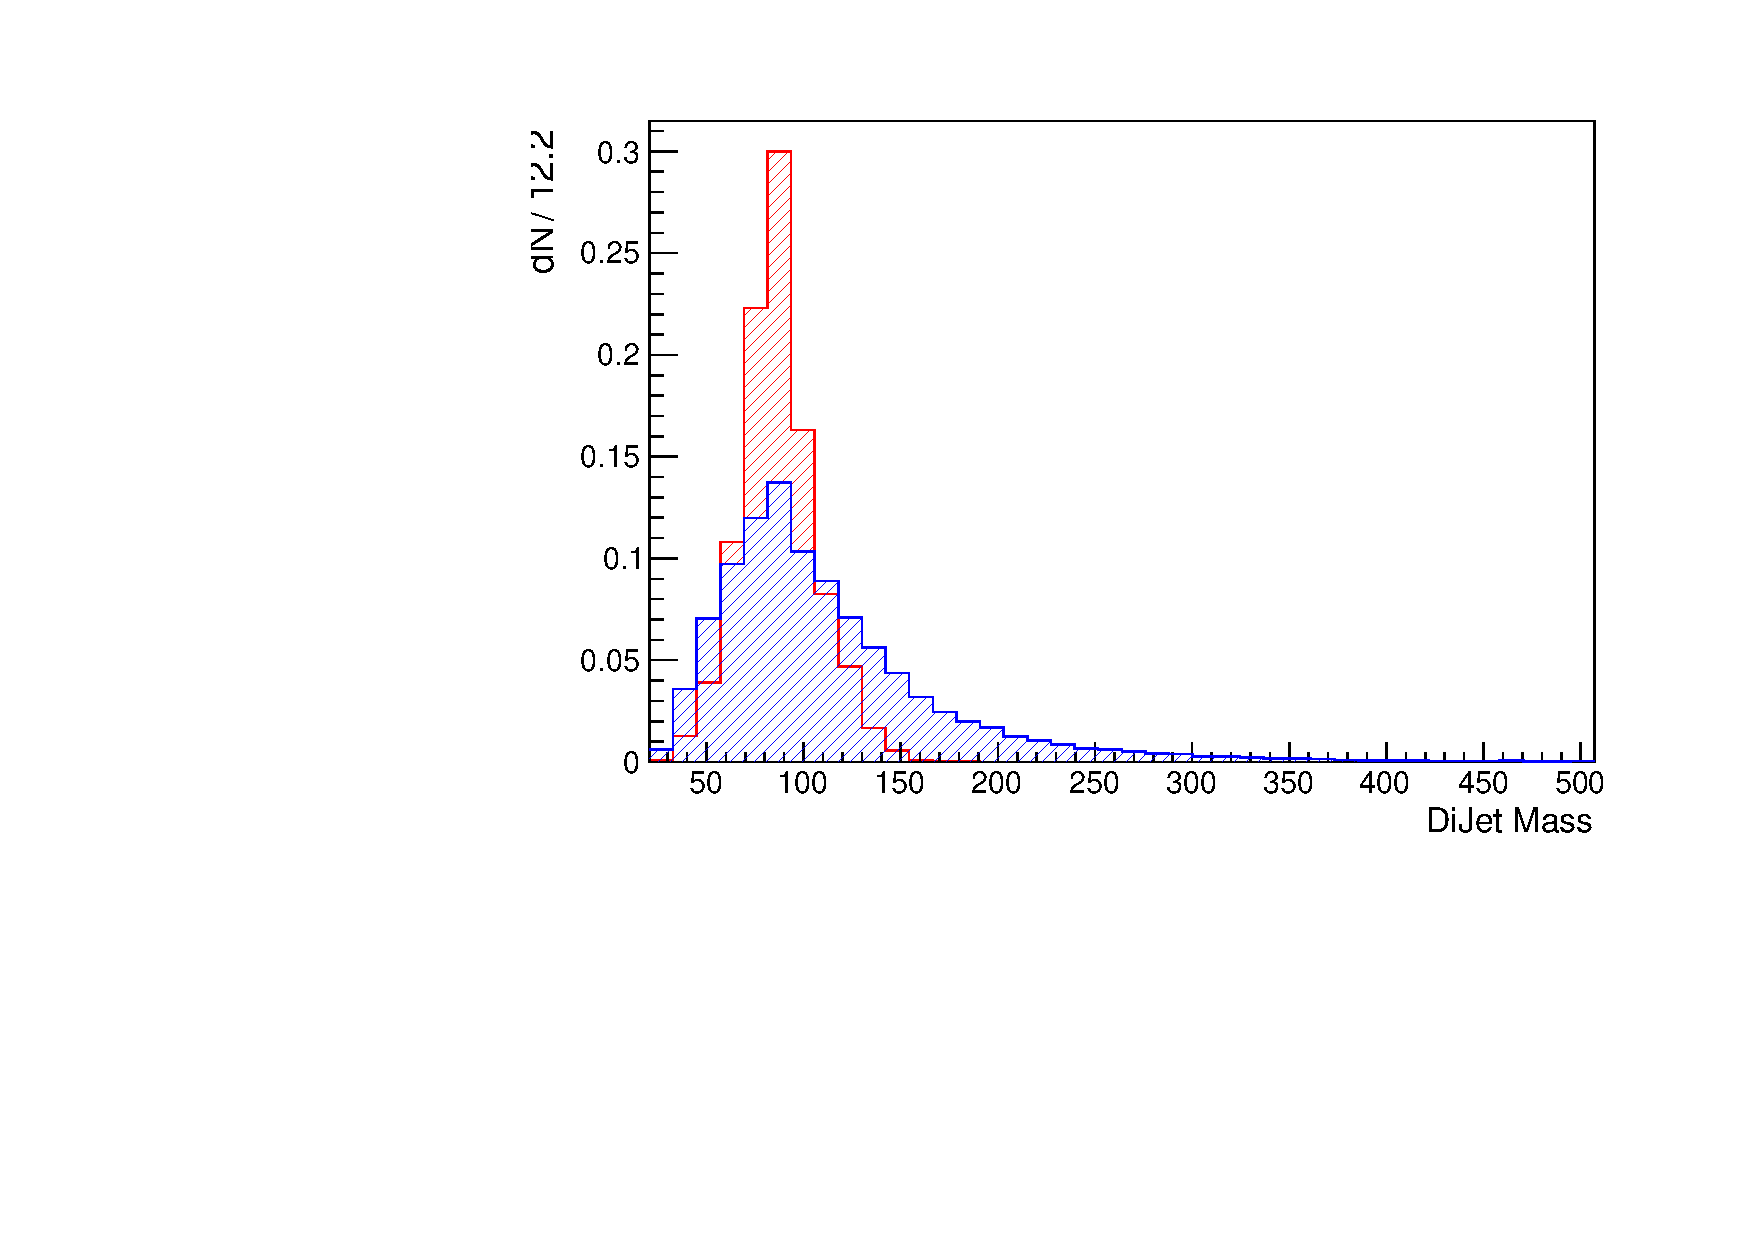
\includegraphics[width=0.49\textwidth]{images/Run1/HadWMass.pdf}
    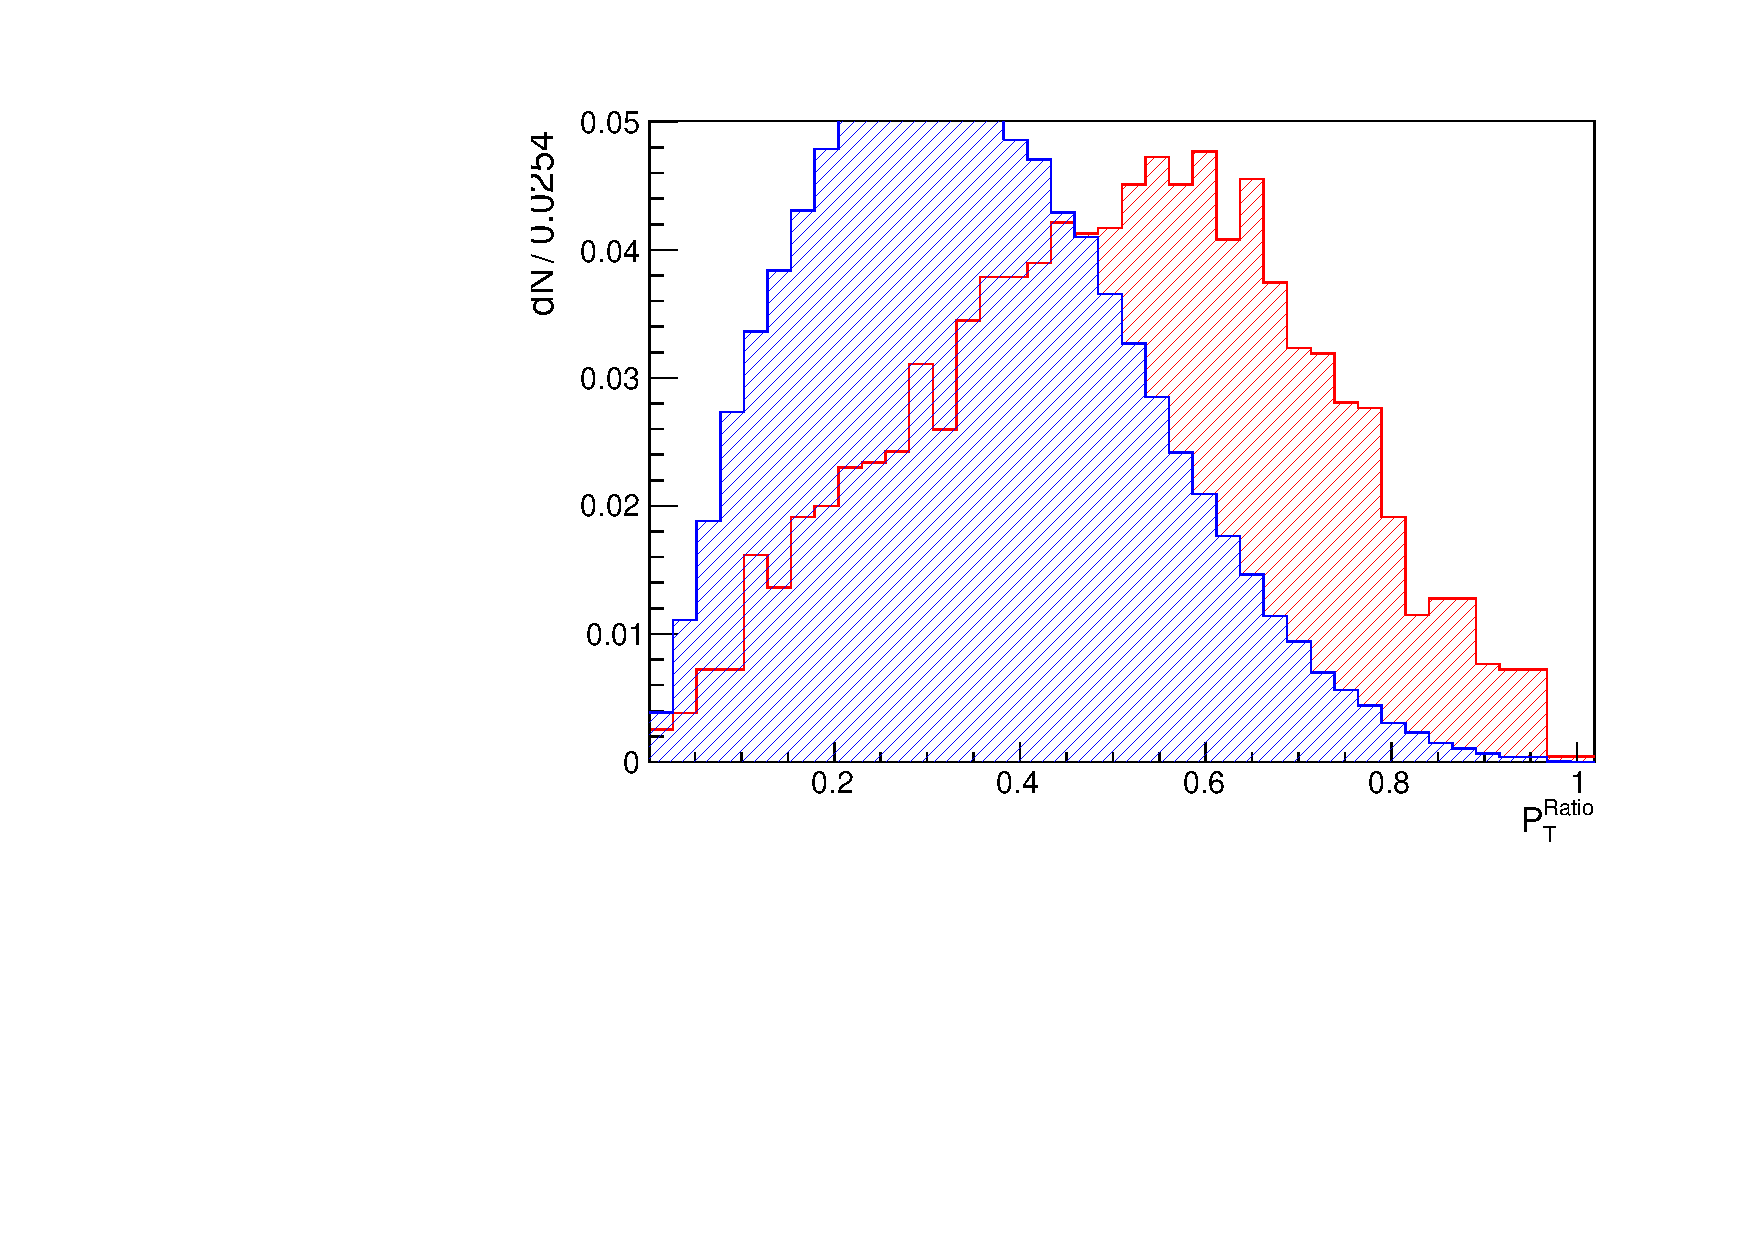
\includegraphics[width=0.49\textwidth]{images/Run1/ThSumPTVecPT.pdf}
     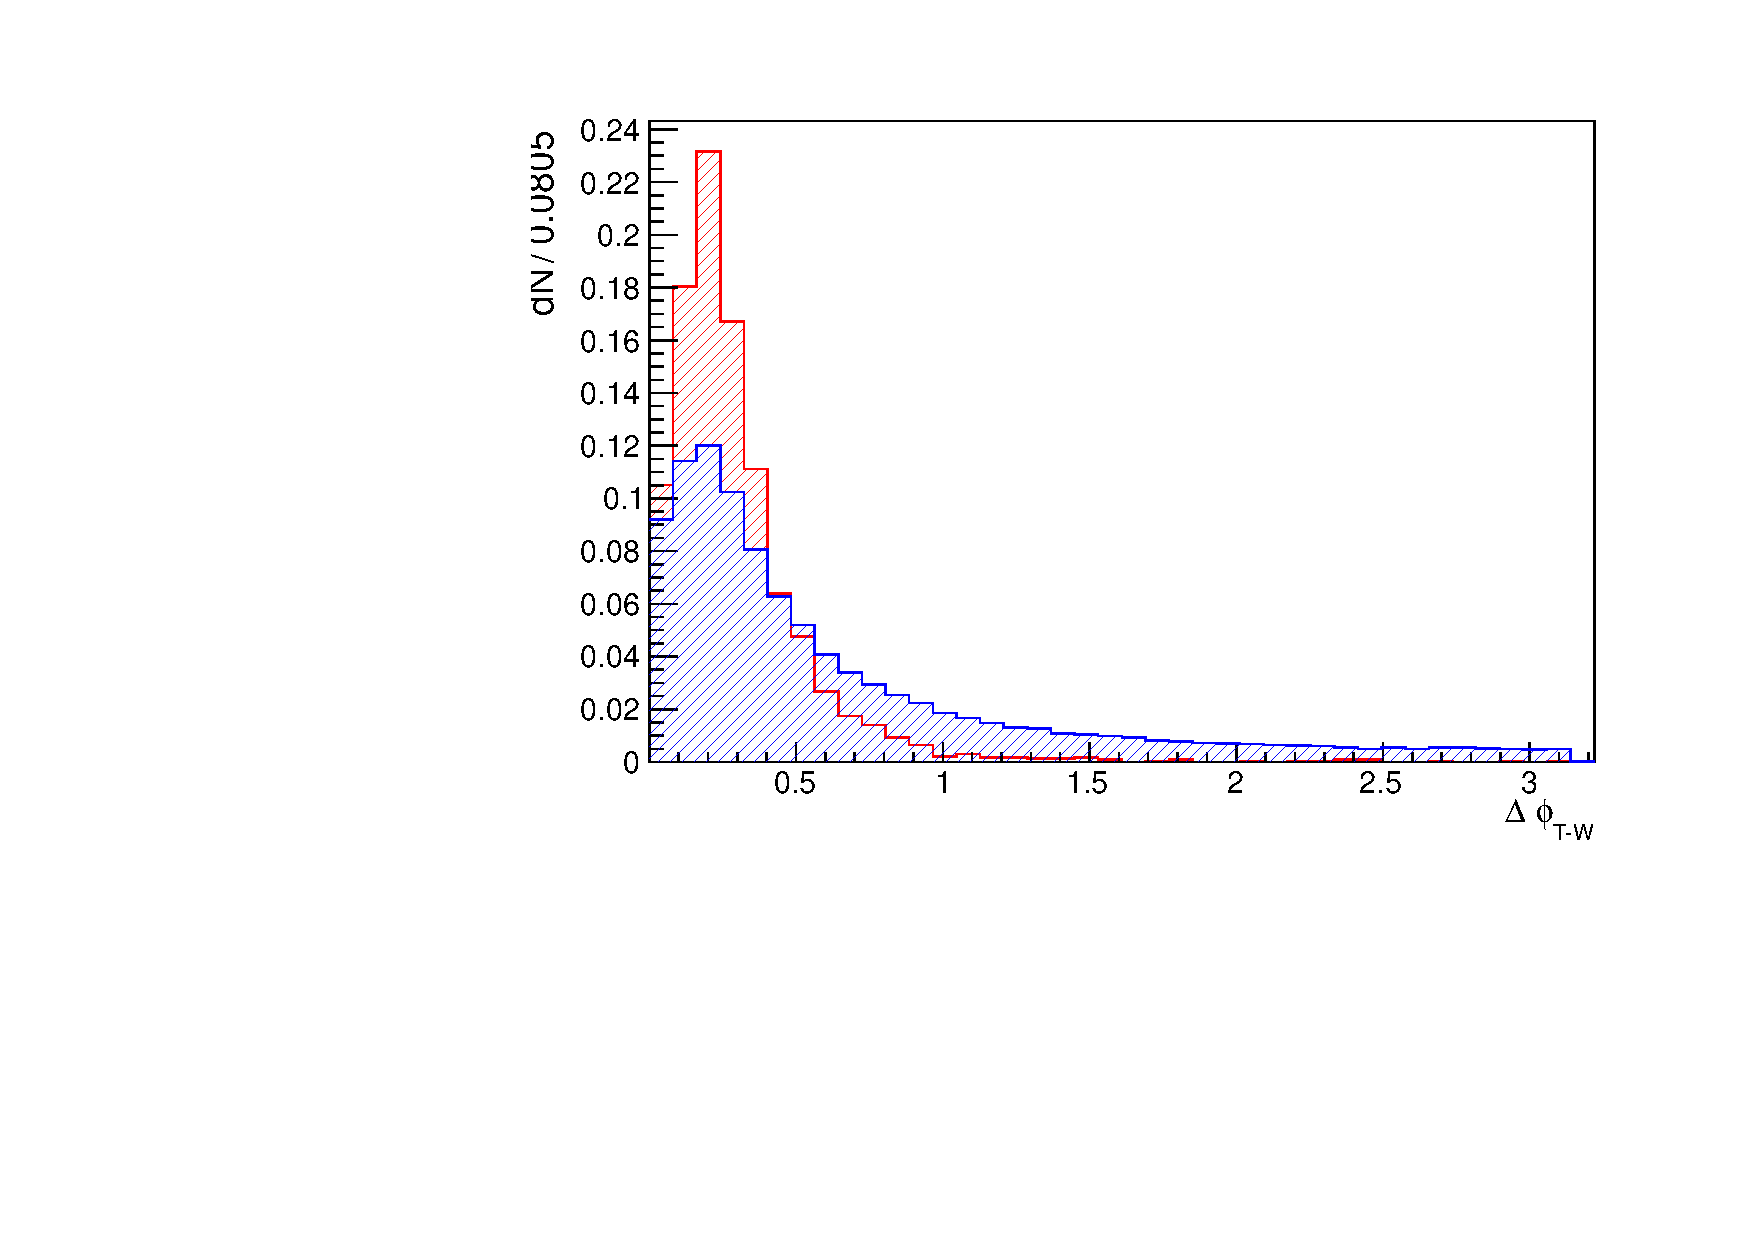
\includegraphics[width=0.49\textwidth]{images/Run1/AnThWh.pdf}
    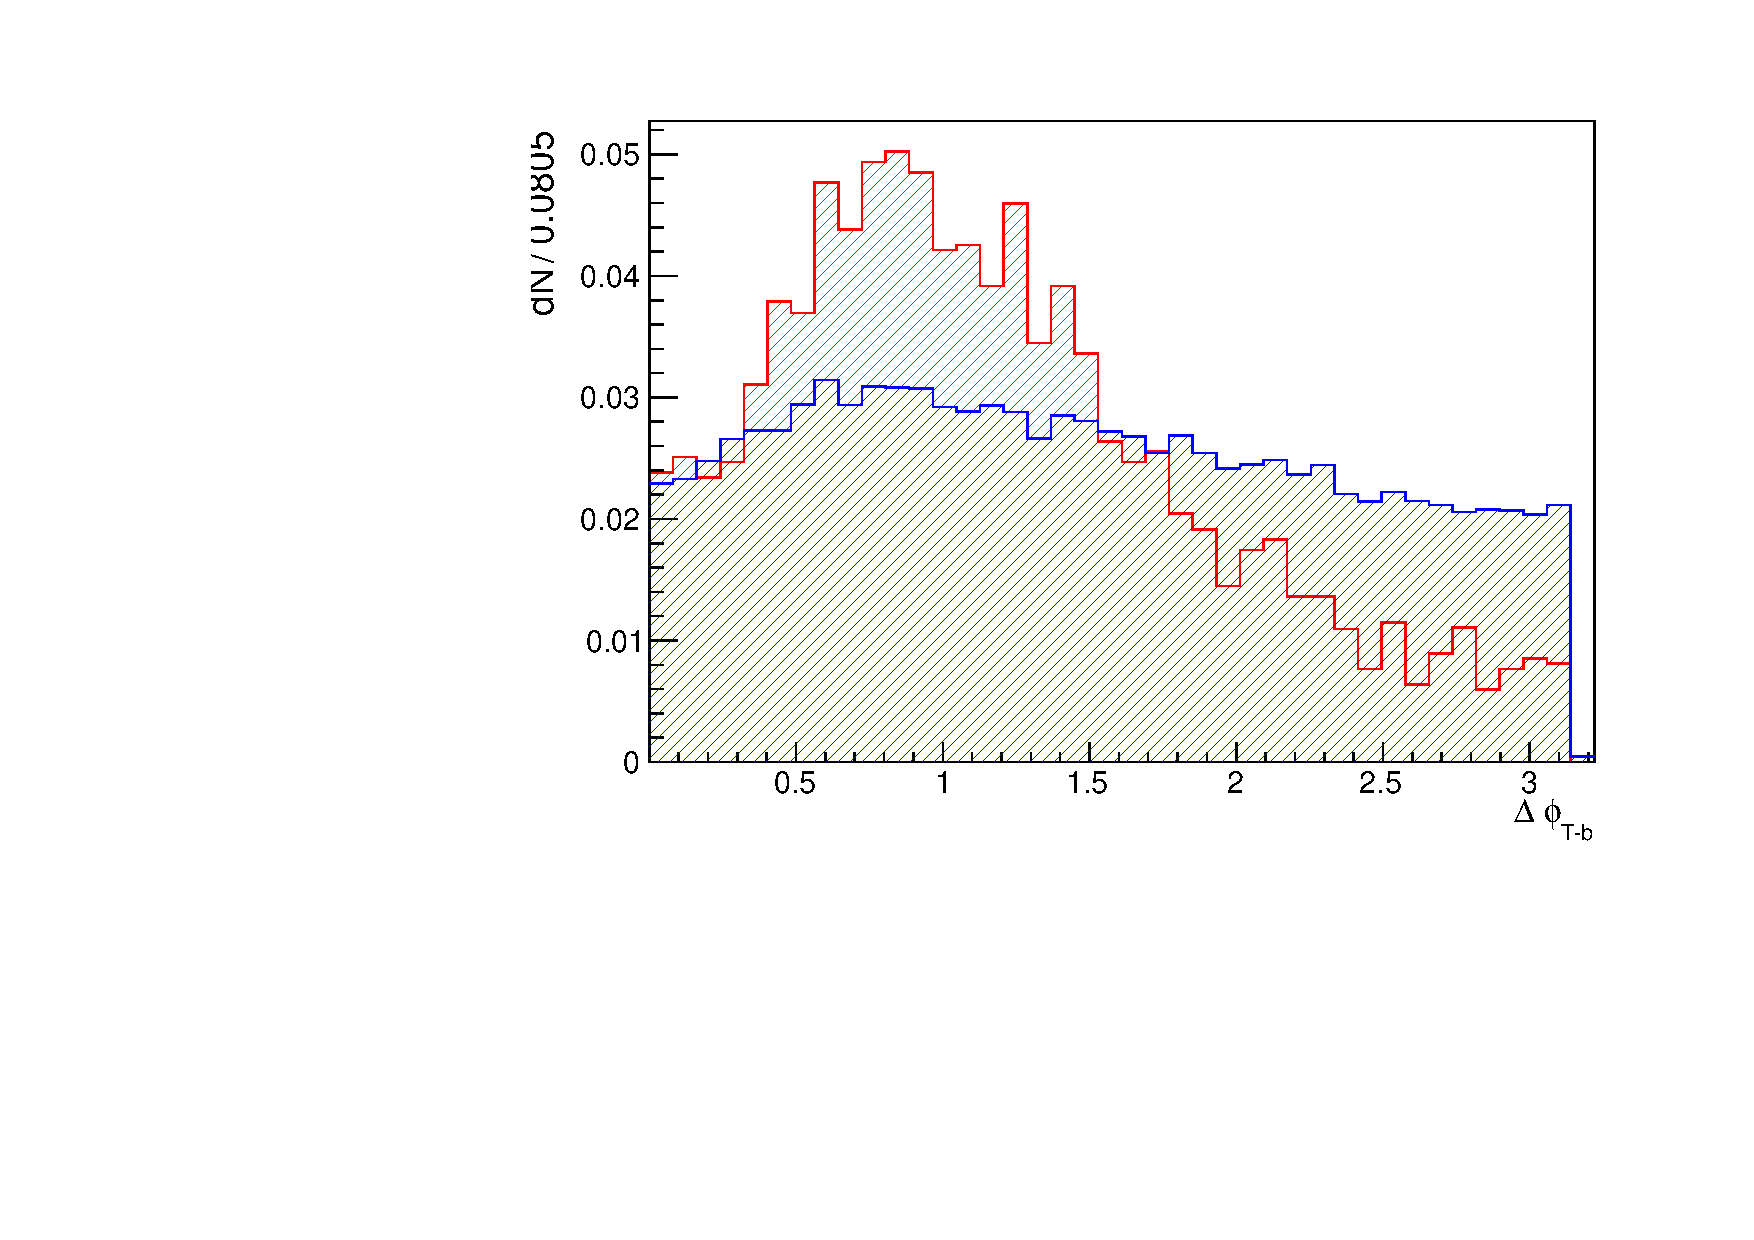
\includegraphics[width=0.49\textwidth]{images/Run1/AnThBh.pdf}
     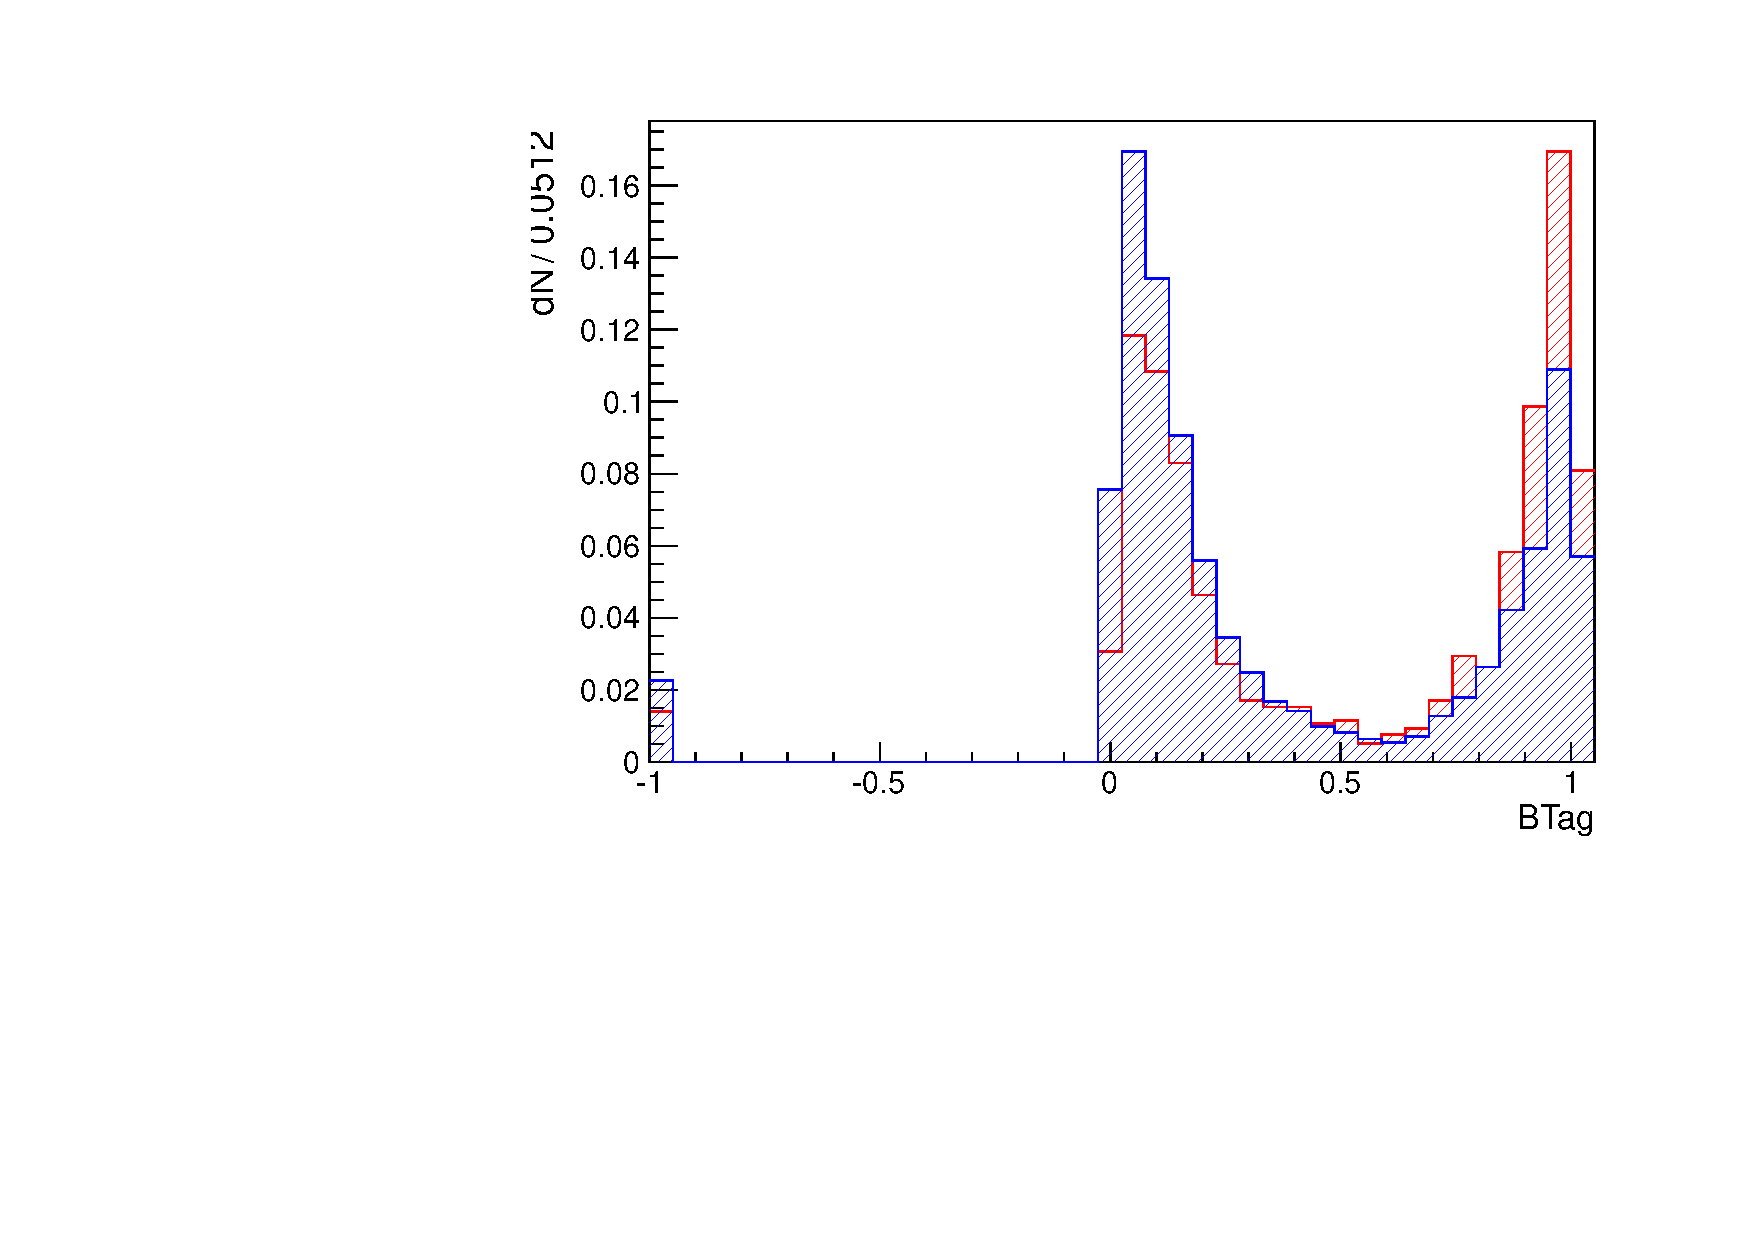
\includegraphics[width=0.49\textwidth]{images/Run1/BTag.pdf}          
    \caption{Input variables into top quark reconstruction BDT.}
    \label{fig:TopBDTinput}
\end{figure}

The multi-variate analysis tool chosen to calculate a variable to discriminate between good and bad tri-jet combinations is a BDT. The BDT is described in more detail in Section~\ref{sec:BDT}. The distribution of the discriminator variable which is output from the BDT is shown in Fig.~\ref{fig:TopBDToutput} where the features in the shape are caused by the large discriminating power of the tri-jet and di-jet invariant mass.
\begin{figure}[!ht]
\centering
    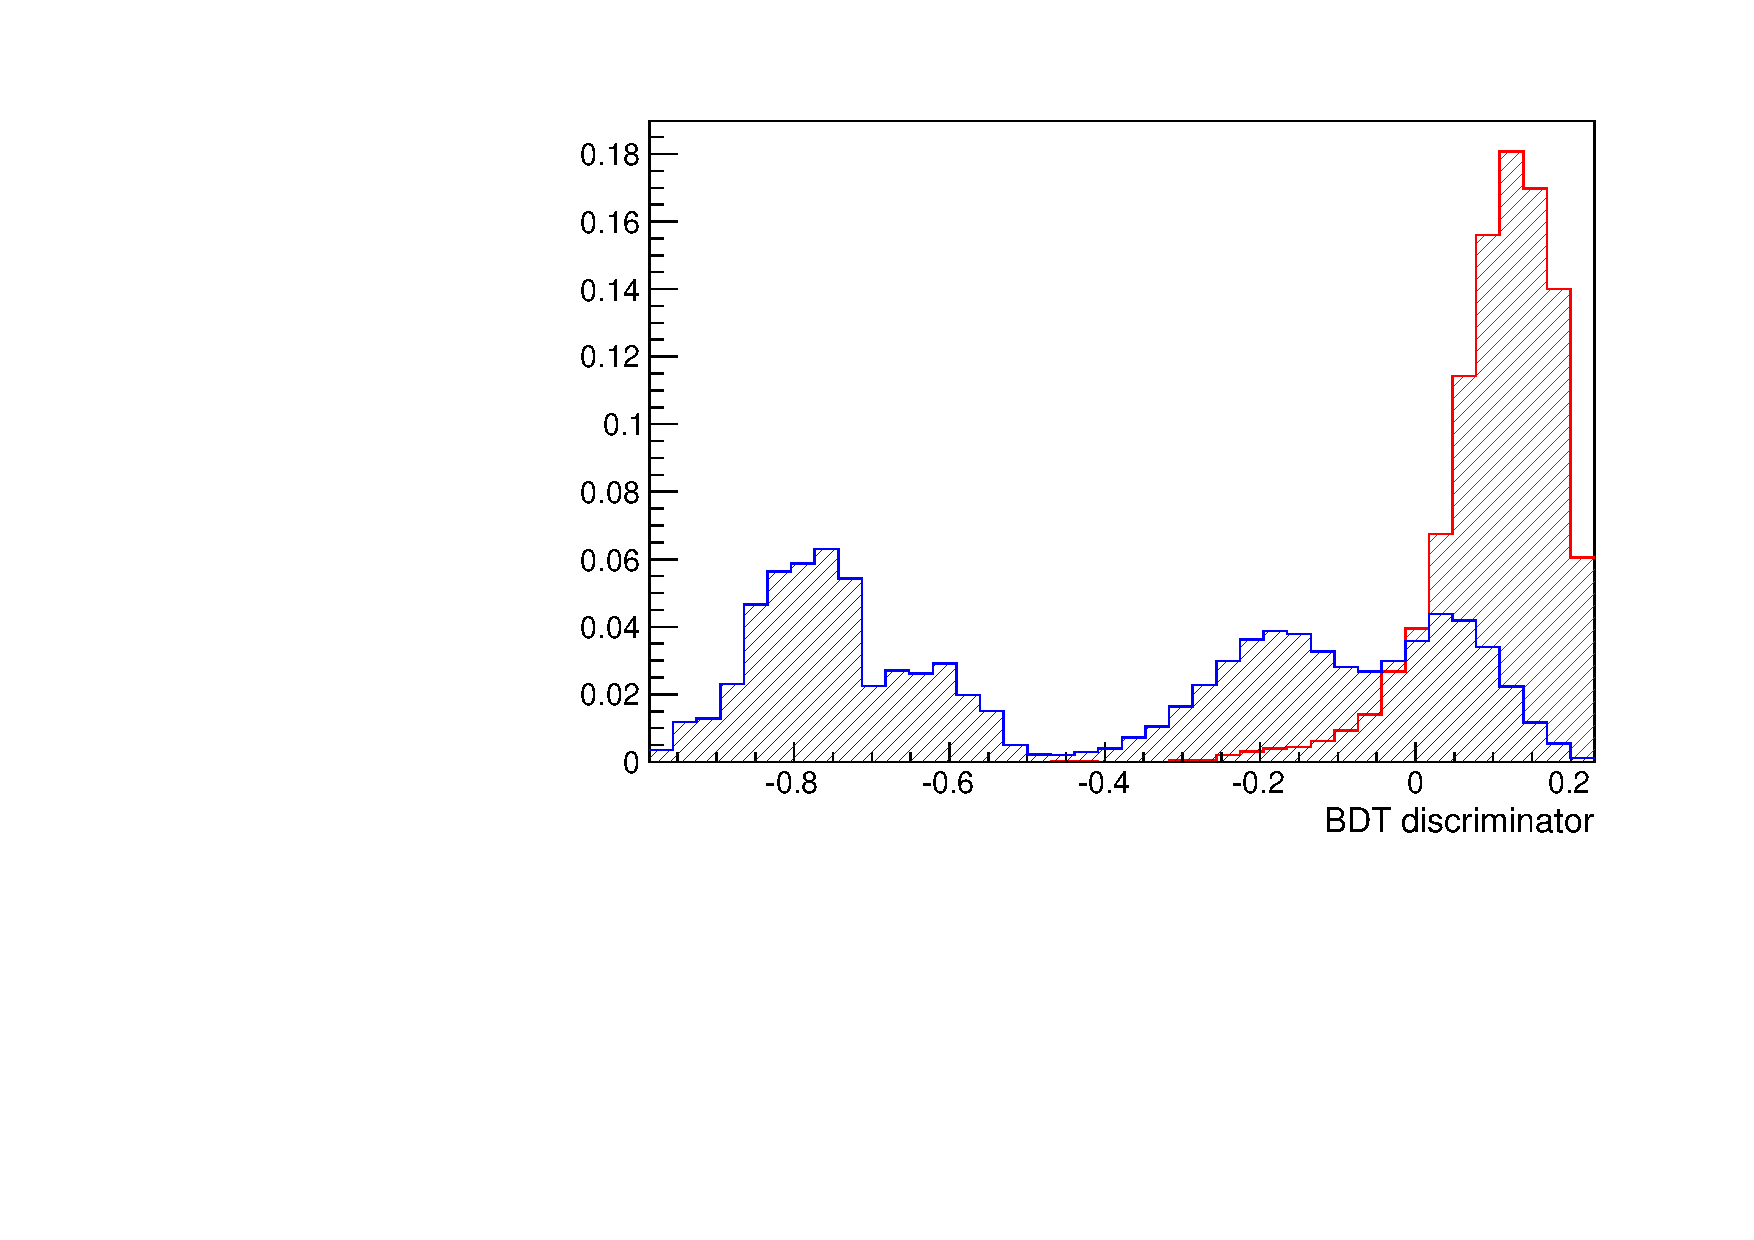
\includegraphics[width=0.6\textwidth]{images/Run1/BDT_Disc.pdf}
    \caption{Output discriminator variable from top quark reconstruction BDT}
    \label{fig:TopBDToutput}
\end{figure}

\subsubsection*{Multitopness}
Multitopness is defined to be the BDT discriminator value of the second highest ranking tri-jet after the first highest-ranking tri-jet has been removed from the collection and the remaining jets have been passed through the BDT again. The multitopness value should have values close to 1 for events where there is a second reconstructible top and a value close to -1 where there is only one reconstructible top which has been removed from the collection and the remaining jets are from ISR or FSR. The distributions of the multitopness variable are shown in Fig.~\ref{fig:Multitopness} for the muon and electron channel. It can be seen that the data and simulation agree well and there is some difference between the shape of the signal and background distributions. The interesting features in the distributions shape come from the the BDT. The two strongest variables, the tri-jet invariant mass and the di-jet invariant mass, split the dataset sharply into two and then four main sections.

\begin{figure}[!ht]
    \includegraphics[width=0.49\textwidth]{images/Run1/MultiTopness_Mu.pdf}
    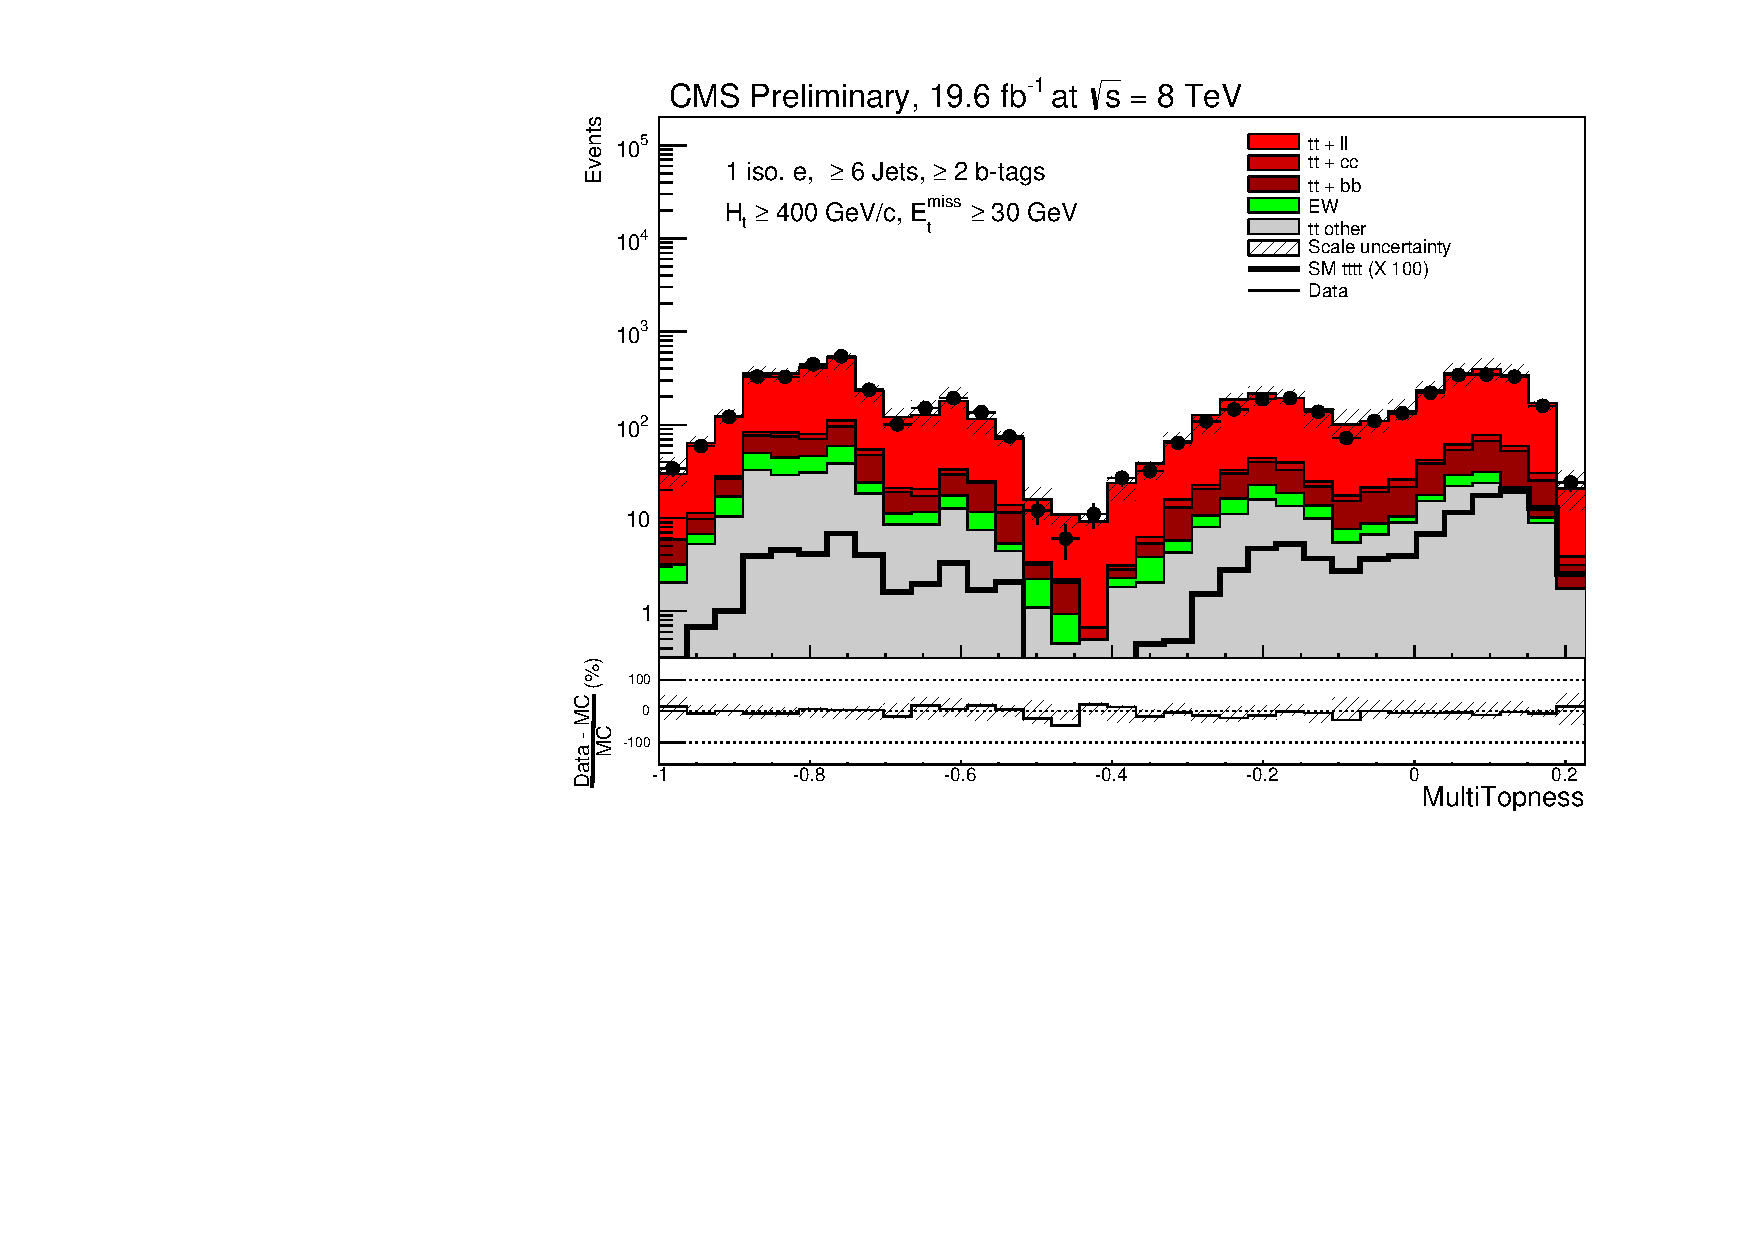
\includegraphics[width=0.49\textwidth]{images/Run1/MultiTopness_e.pdf}
    \caption{Multitopness variable in data and simulation for $\mu$ + jets (right) and e + jets (left).}
    \label{fig:Multitopness}
\end{figure}

\subsubsection*{Reduced Event Variables}
New event variables are constructed from removing the highest ranking tri-jet from the jets collection to created a reduced event. These reduced event variables exploit the fact the \ttbar events should only have softer jets remaining from ISR and FSR, whereas \tttt events should have ore energetic jets from the two additional hadronic top quarks.

\textbf{\HTX} - This is the \HT of the reduced event.\\
\textbf{\sumjetmassX} - Invariant mass of all jets contained in the reduced event.

Plots for these reduced event variables can be seen in Figs~\ref{fig:HTX},~\ref{fig:sumjetmassX}.

\begin{figure}[!ht]
    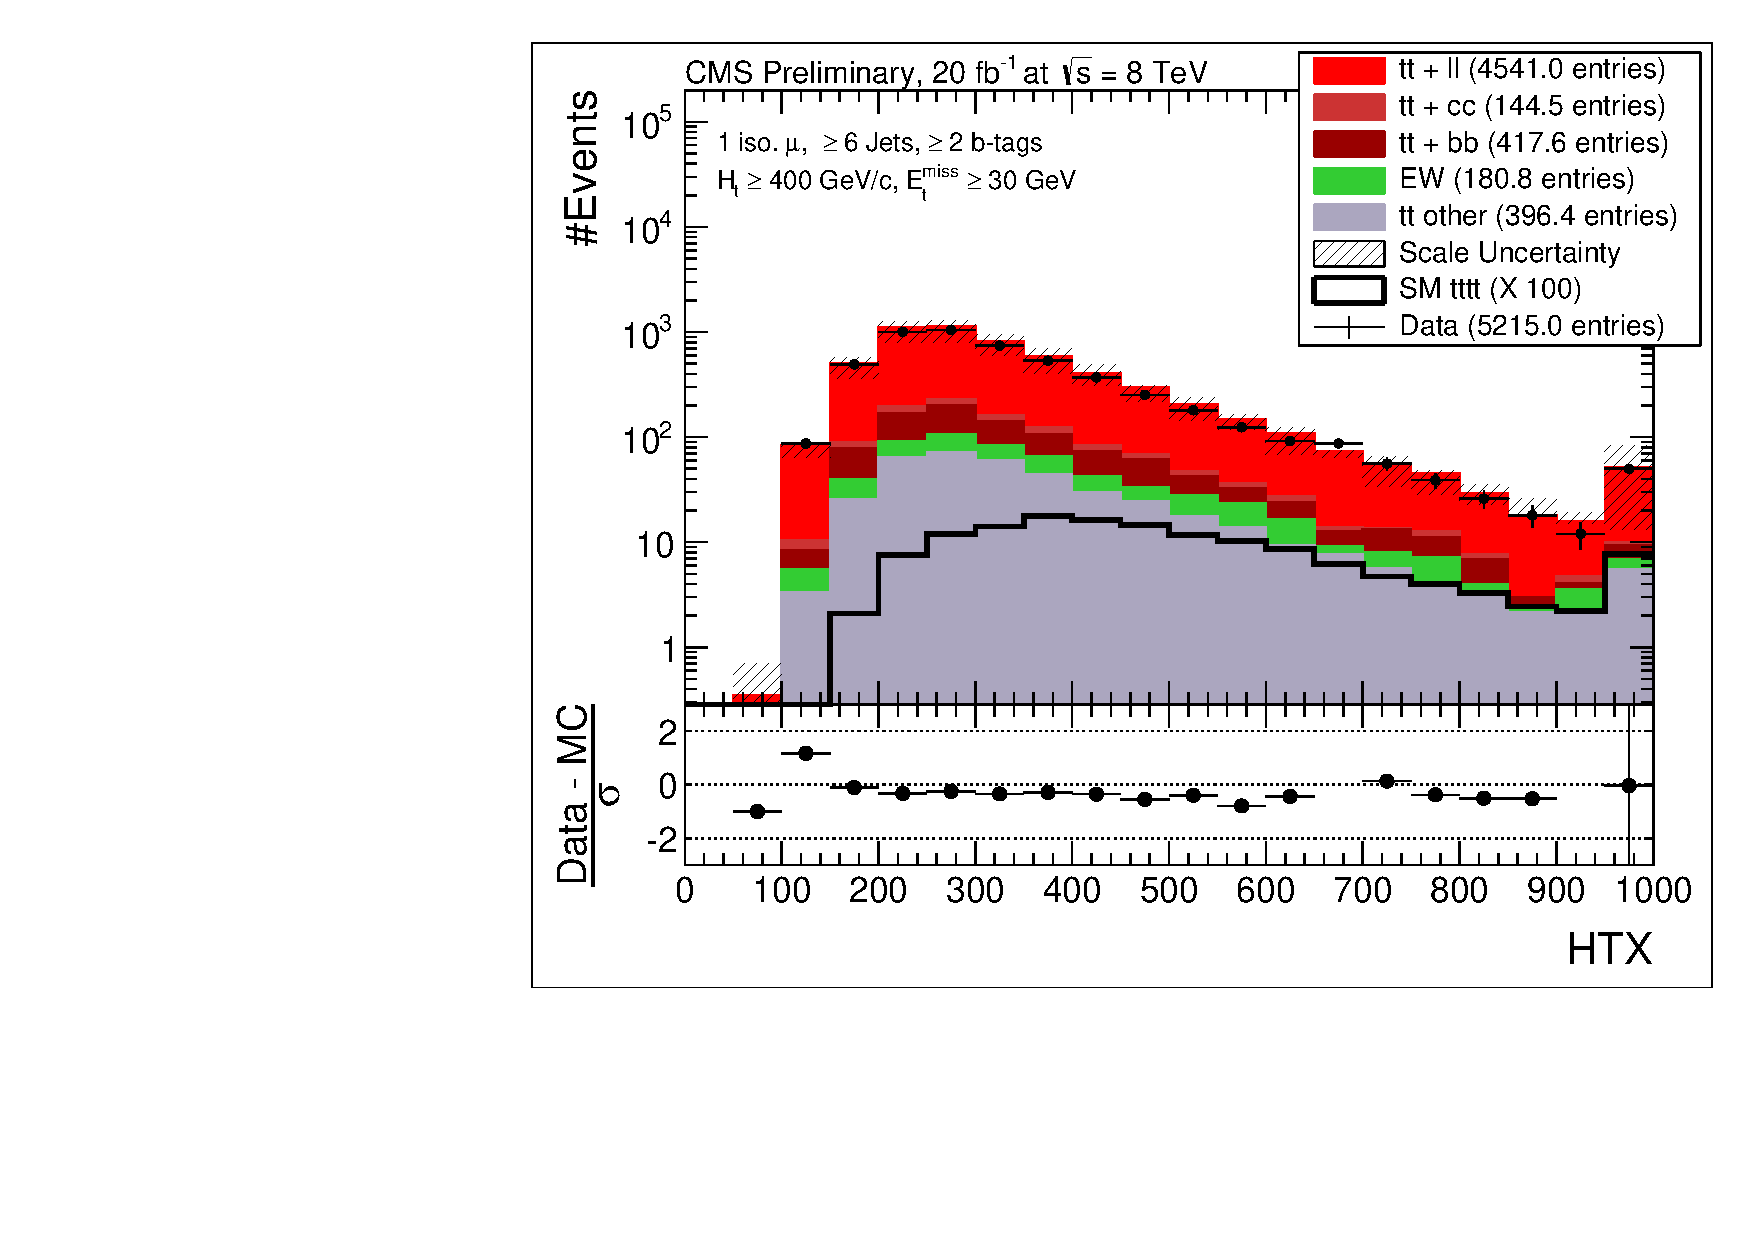
\includegraphics[width=0.49\textwidth]{images/Run1/HTX_StackLogY_Mu.pdf}
    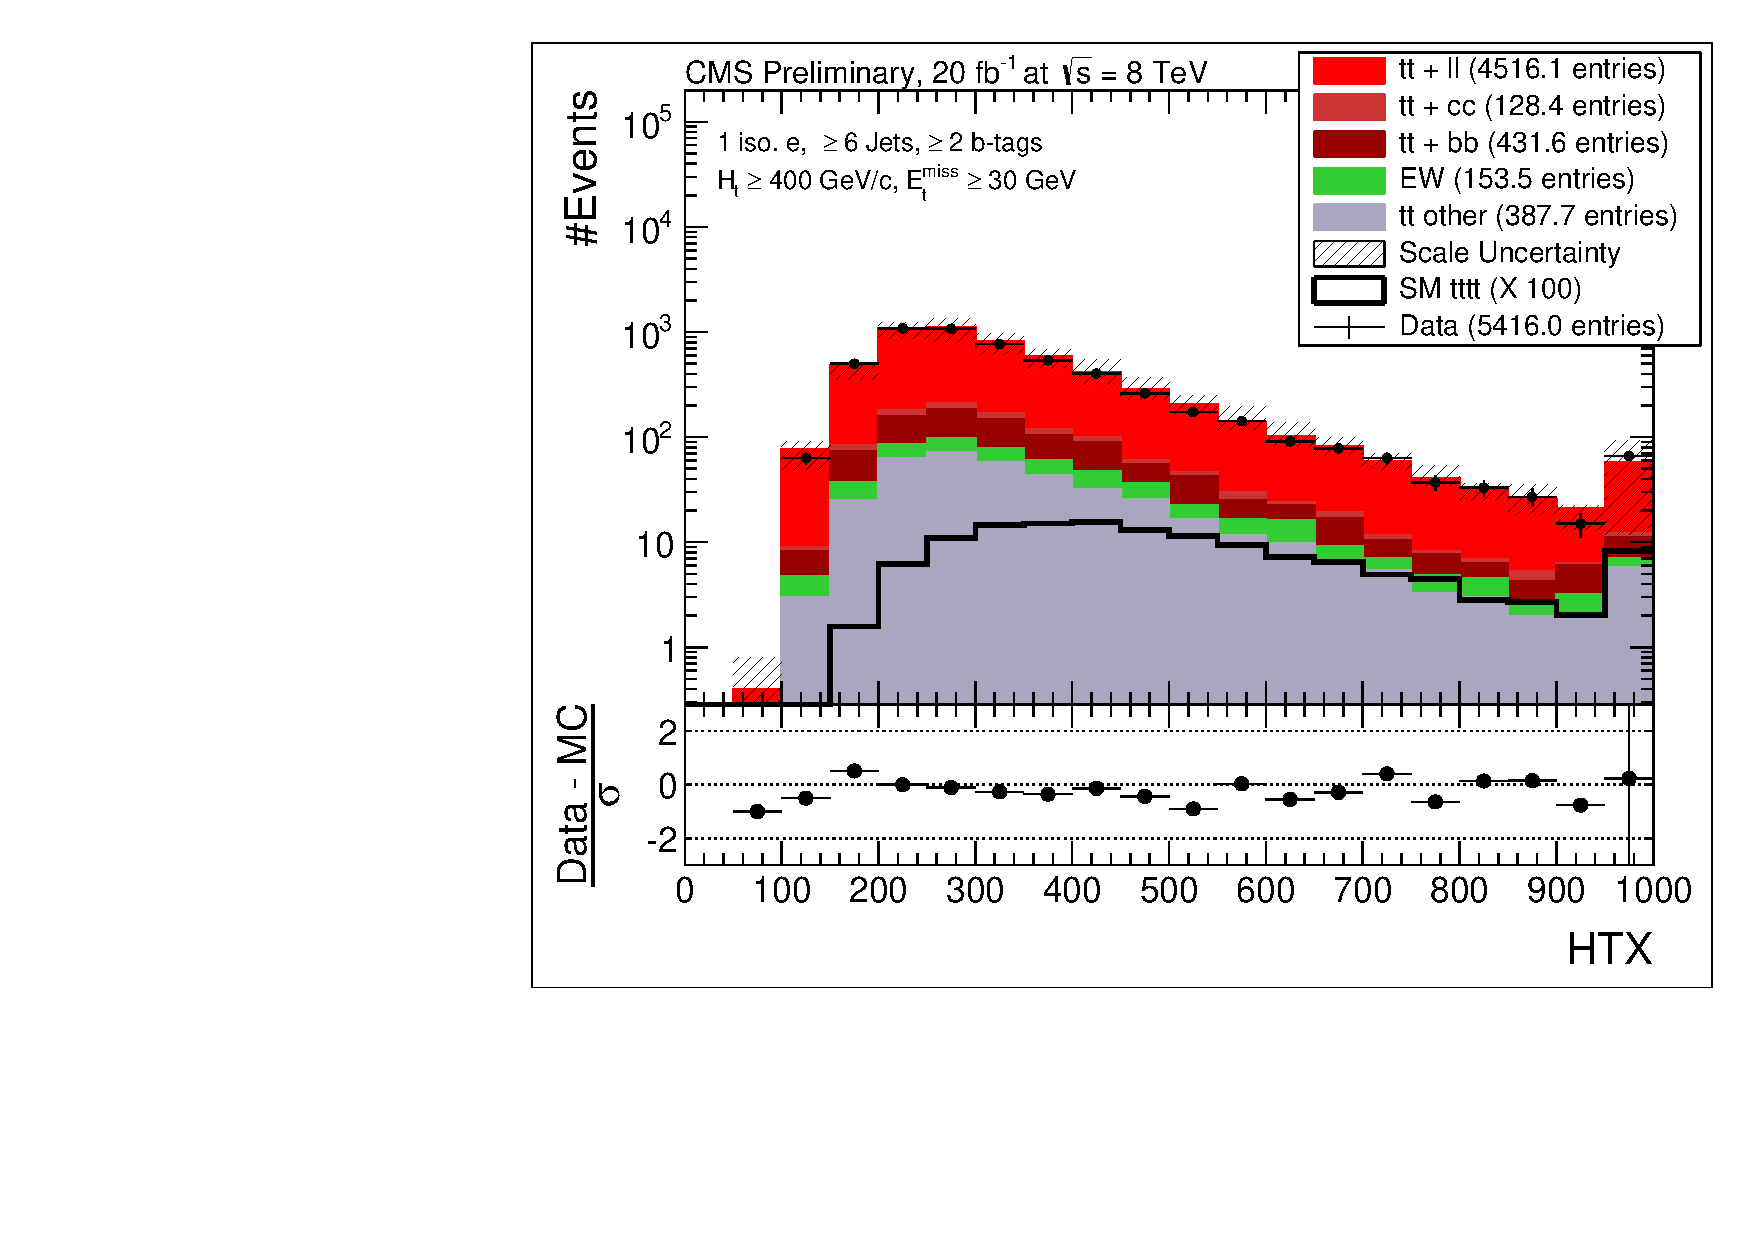
\includegraphics[width=0.49\textwidth]{images/Run1/HTX_StackLogY_e.pdf}
    \caption{\HTX for $\mu$ + jets (right) and e + jets (left).}
    \label{fig:HTX}
\end{figure}

\begin{figure}[!ht]
    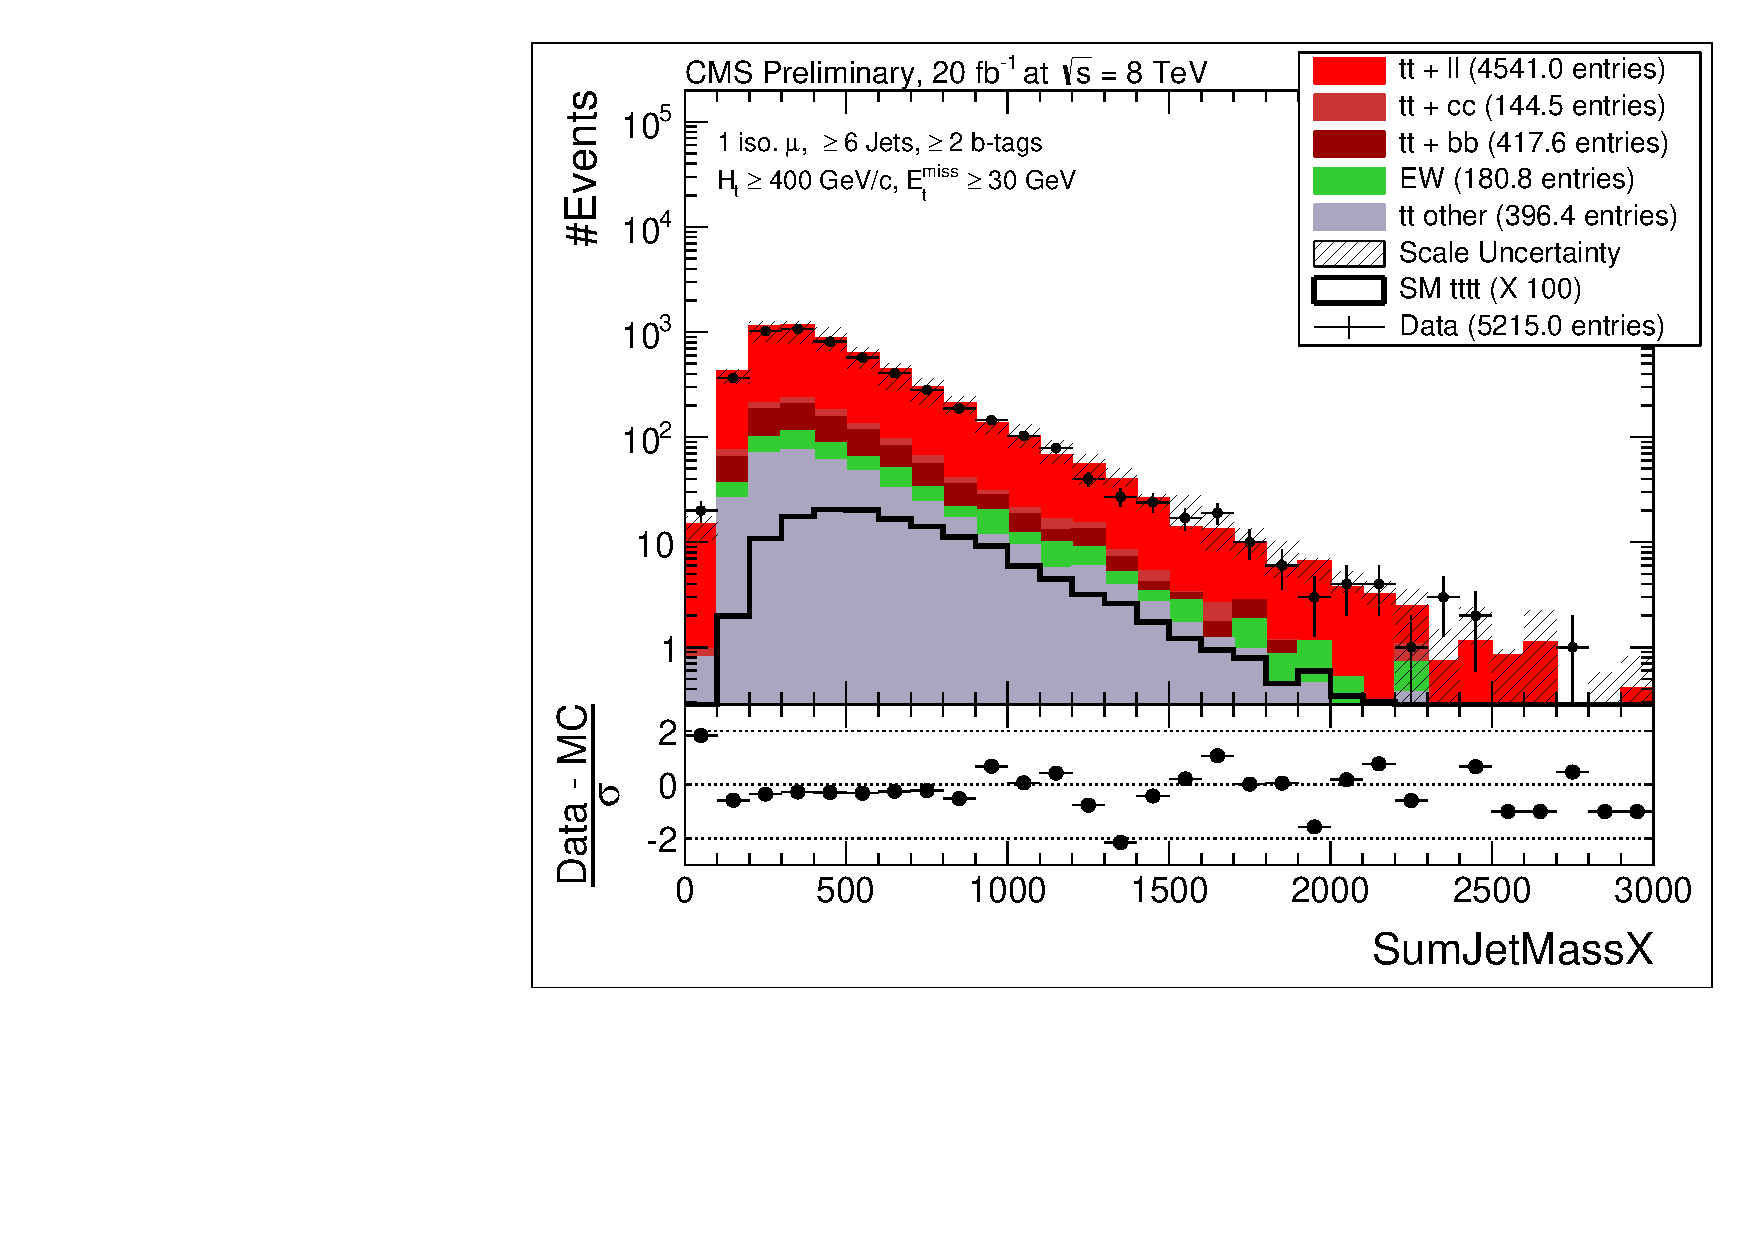
\includegraphics[width=0.49\textwidth]{images/Run1/SumJetMassX_StackLogY_Mu.pdf}
    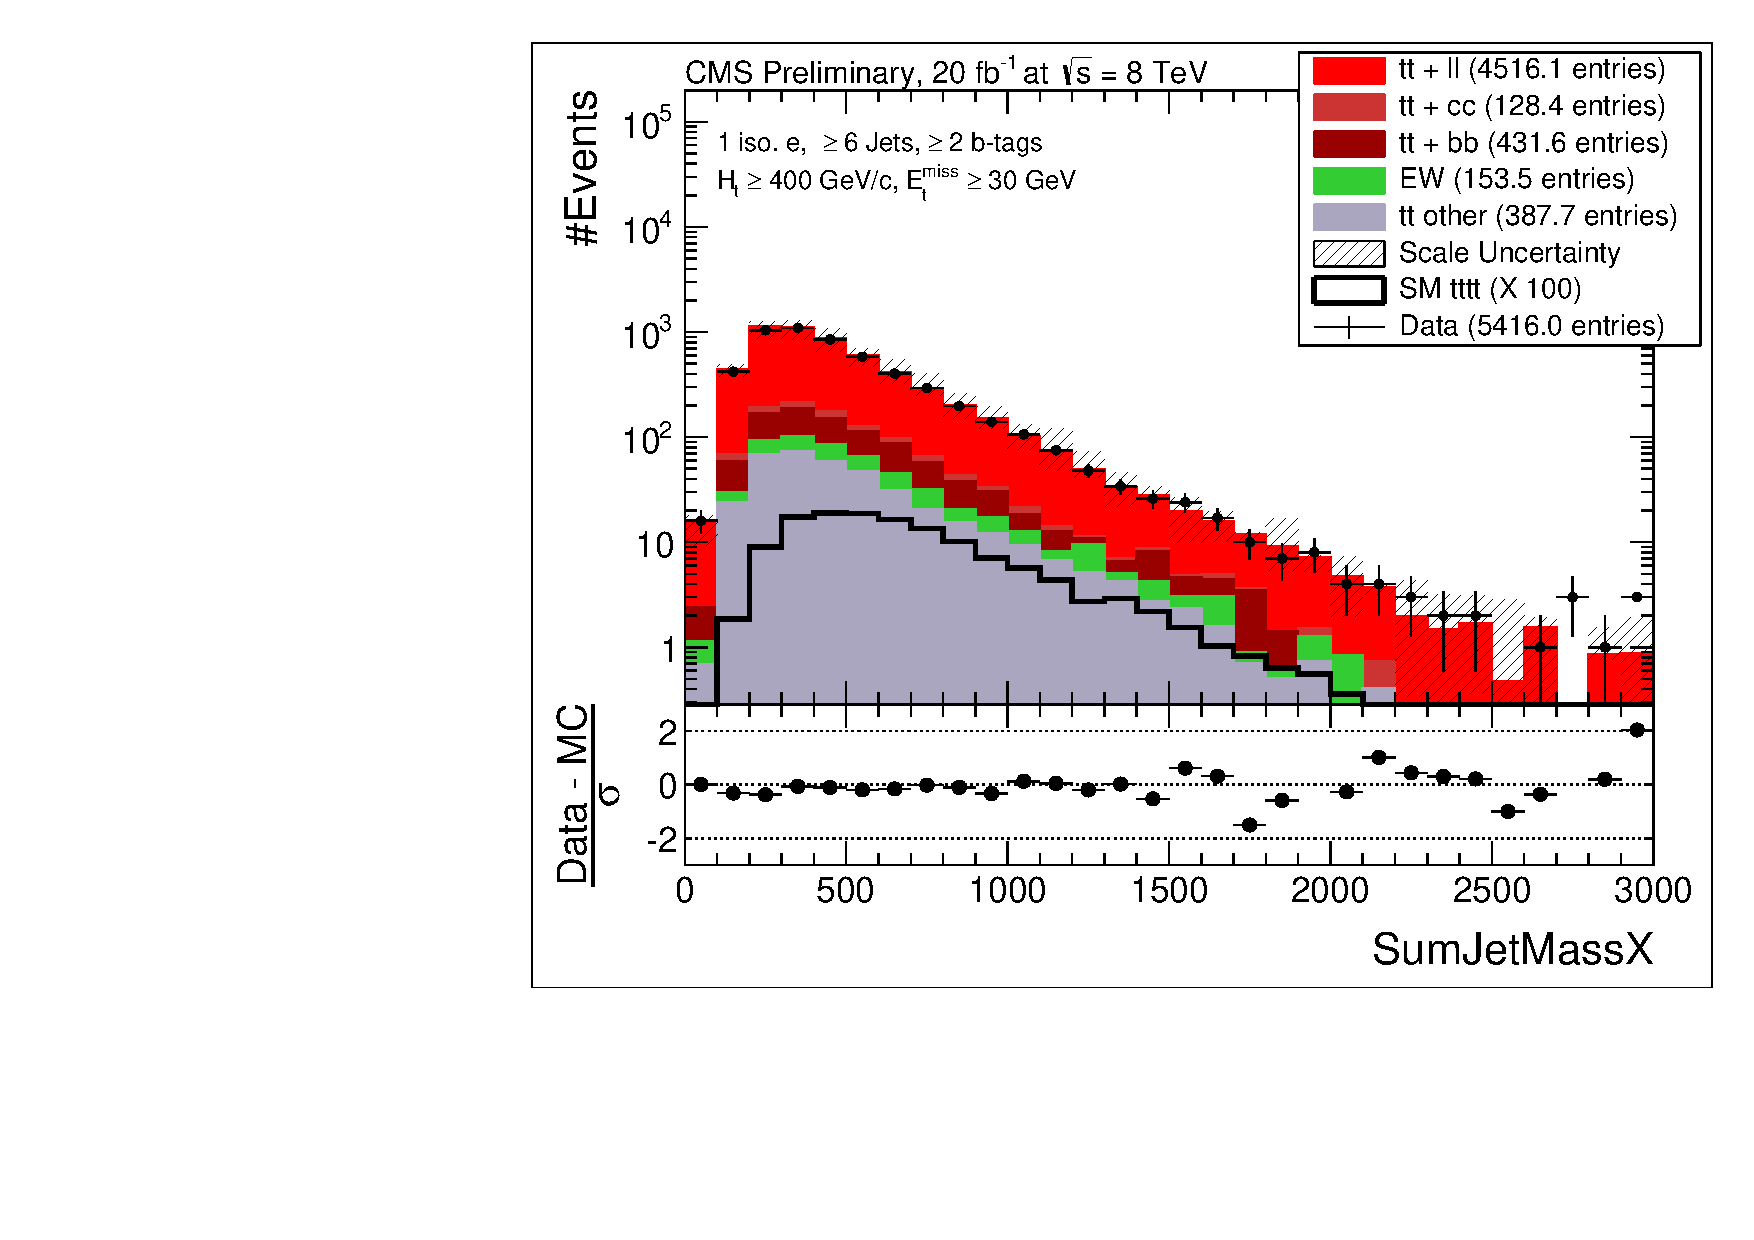
\includegraphics[width=0.49\textwidth]{images/Run1/SumJetMassX_StackLogY_e.pdf}
    \caption{\sumjetmassX for $\mu$ + jets (right) and e + jets (left).}
    \label{fig:sumjetmassX}
\end{figure}

\subsection{b-jet content}
\label{sec:bottomContent}
Top quarks decay almost exclusively into bottom quarks by \cPqt $\rightarrow$ \cPqb \Wplus or \cPaqt $\rightarrow$ \cPaqb \Wminus. Therefore, it should be possible to use the number of bottom quarks in the event to distinguish between \tttt events, which should have four bottom quarks in comparison to \ttbar + jets events which typically have two bottom quarks. However this variable does not help to distinguish between \tttt and \ttbb as \ttbb will also have four bottom quarks in the final state. Also \ttbar + jets may have additional bottom quarks arising from the ISR or FSR. Fig~\ref{fig:datasimnbtags} shows the distribution of \nbtags.

\subsection{Event activity}
\label{sec:eventActivity}
Many variables can be derived by utilising the fact that \tttt events can have up to 10 hard jets whereas \ttbar events should only have up to 4 hard jets. This difference in hadronic activity is exploited by forming the following variables:\\
\textbf{\njets} - The number of jets is an obvious variable for distinguishing between \tttt and \ttbar. It can be seen in Fig.~\ref{fig:datasimnjets}. \\
\textbf{\HTb} - The scalar sum of the \pt of the b-tagged jets in the event. Bottom quarks which come from top quark decays tend to have higher \pt than bottom quarks which come from gluon splitting and other processes. As \tttt events should contain four b-quarks which come from top decays and \ttbar events contain two b-quarks from top decays, this variable should be larger for \tttt events, as can be seen in Fig.~\ref{fig:HTb}.\\
\textbf{Centrality} - This is defined as the ratio of the \HT in the event to the H in the event, where H is the scalar sum of the total momentum (P) in the event.\\
\textbf{\HTrat} - This is defined as the ratio of the \HT of the four leading jets to the \HT of the other jets in the event. For \ttbar, which should have only four hard jets, this ratio should be larger than \tttt which should have a value closer to one as the four hardest jets are balanced be additional hard jets in the event. \\
\textbf{5th jet \pt} - After the four leading hard jets in \ttbar, the 5th jet should have, on average, a lower momentum in \ttbar events than in \tttt events. This can be seen in Fig.~\ref{fig:5thjetpt}.\\
\textbf{6th jet \pt} - Again, the \pt of the 6th jet in \ttbar events should be, on average, lower than in \tttt where the 6th jet is still coming from a hard process. This can be seen in Fig.~\ref{fig:6thjetpt}.\\

\begin{figure}[!ht]
    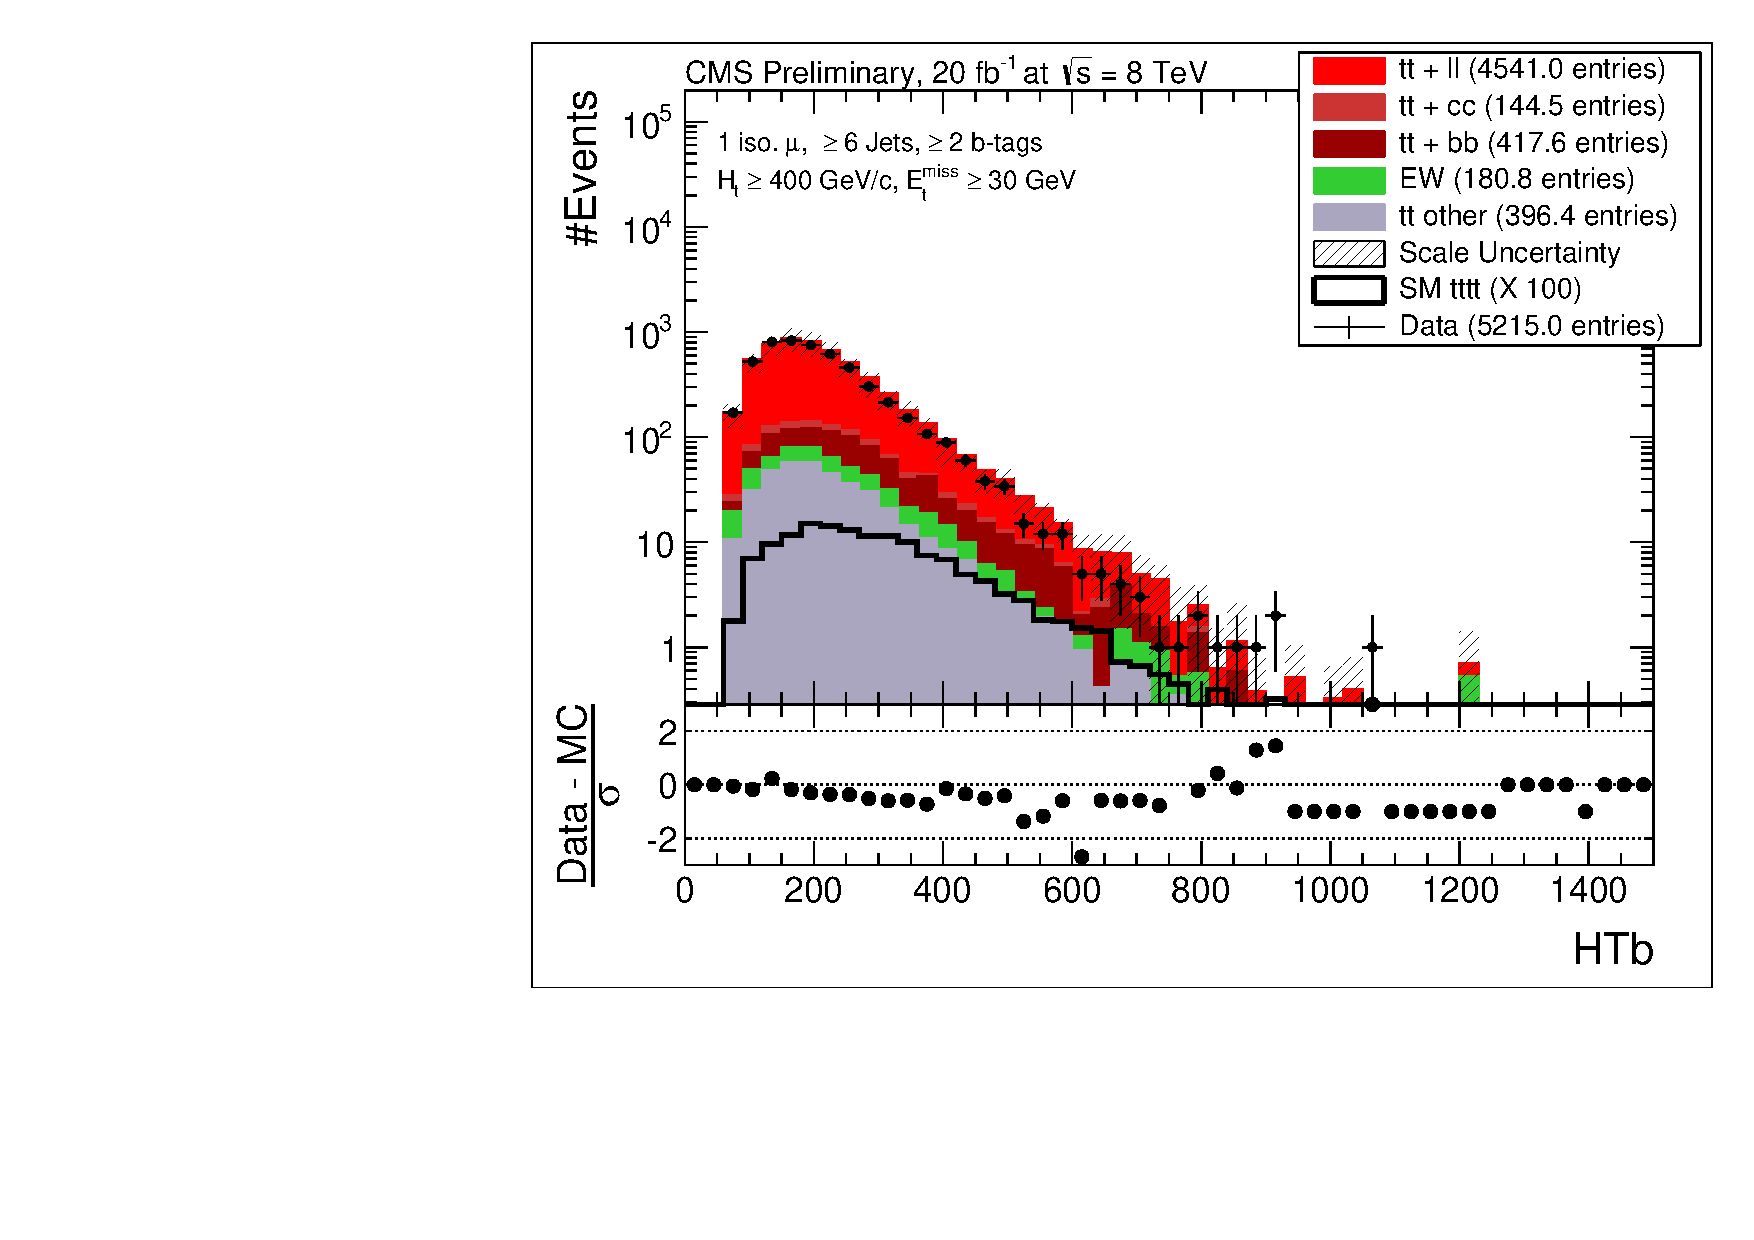
\includegraphics[width=0.49\textwidth]{images/Run1/HTb_SelectedJets_StackLogY_Mu.pdf}
    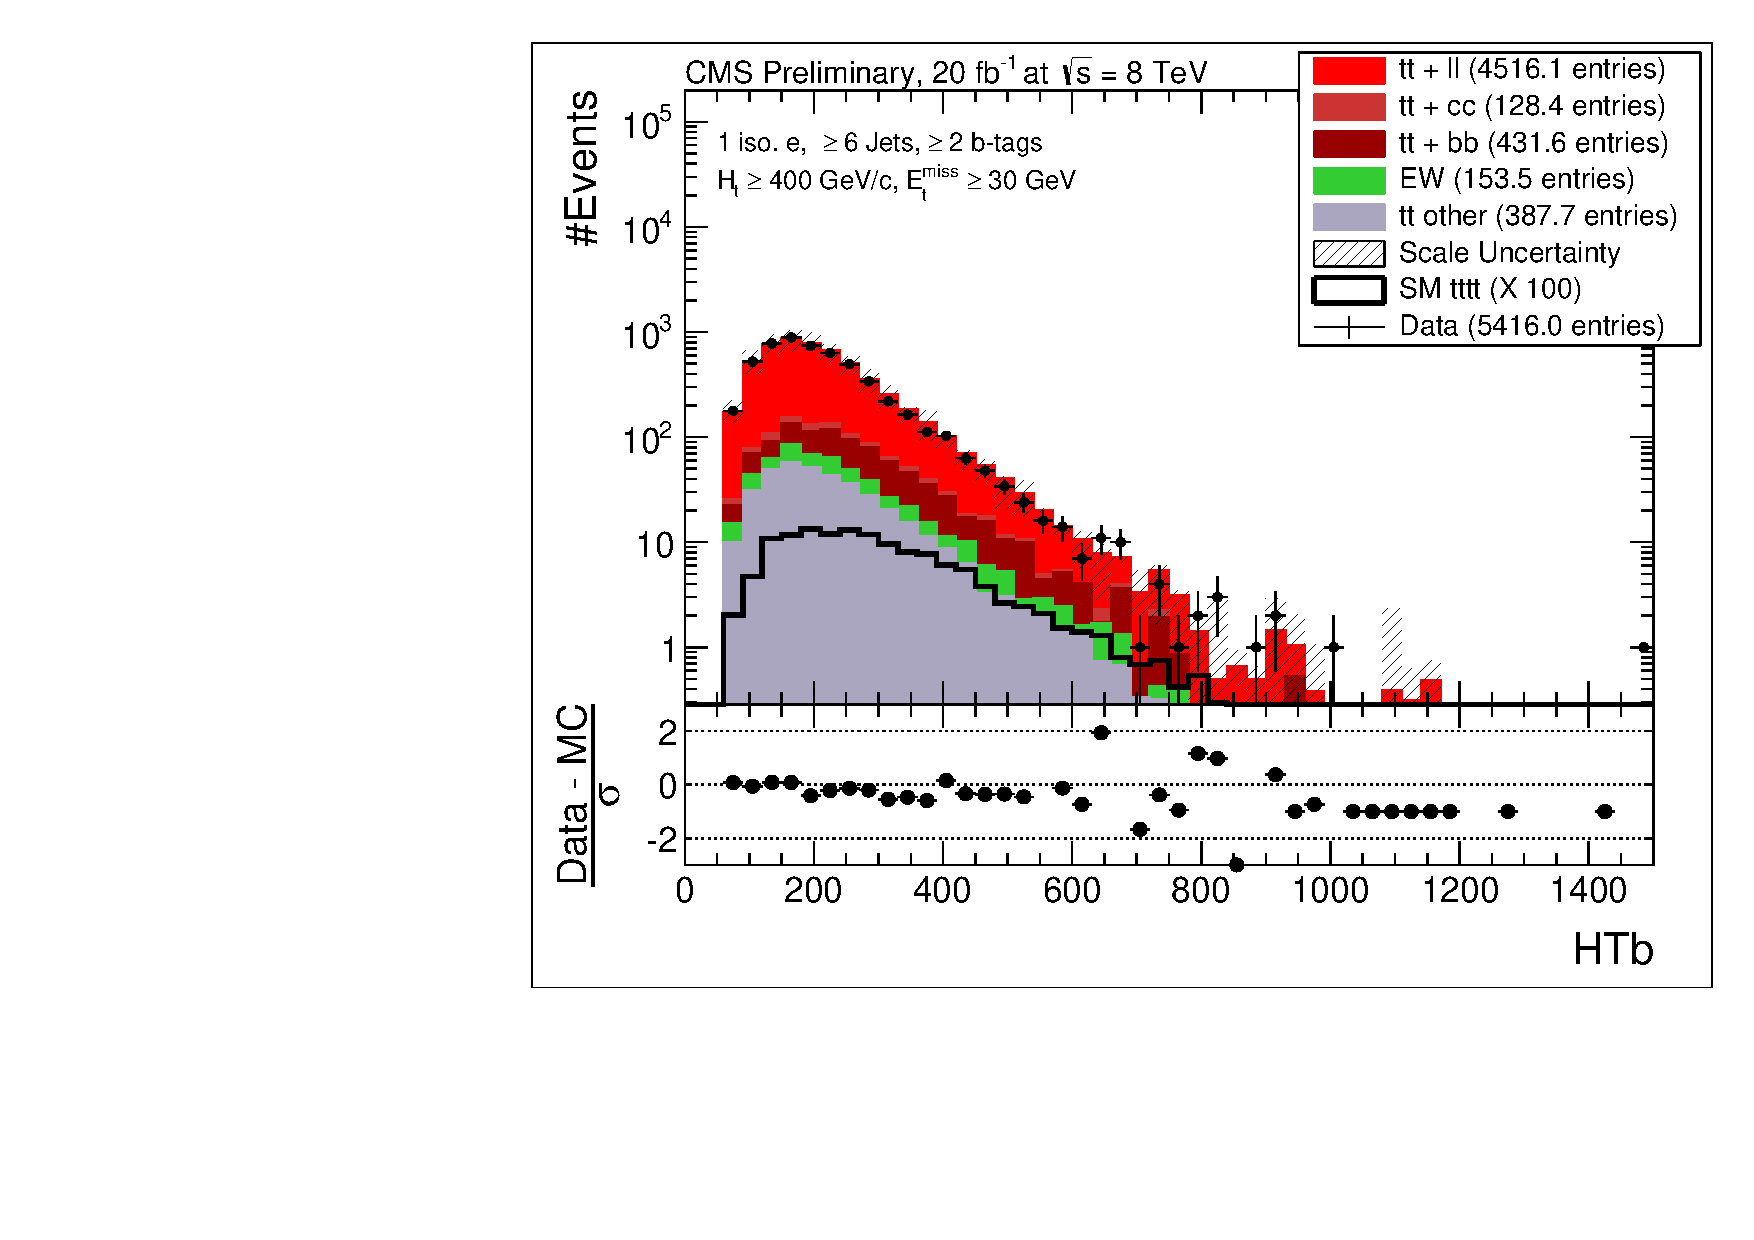
\includegraphics[width=0.49\textwidth]{images/Run1/HTb_SelectedJets_StackLogY_e.pdf}
    \caption{\HTb for $\mu$ + jets (right) and e + jets (left).}
    \label{fig:HTb}
\end{figure}

\begin{figure}[!ht]
    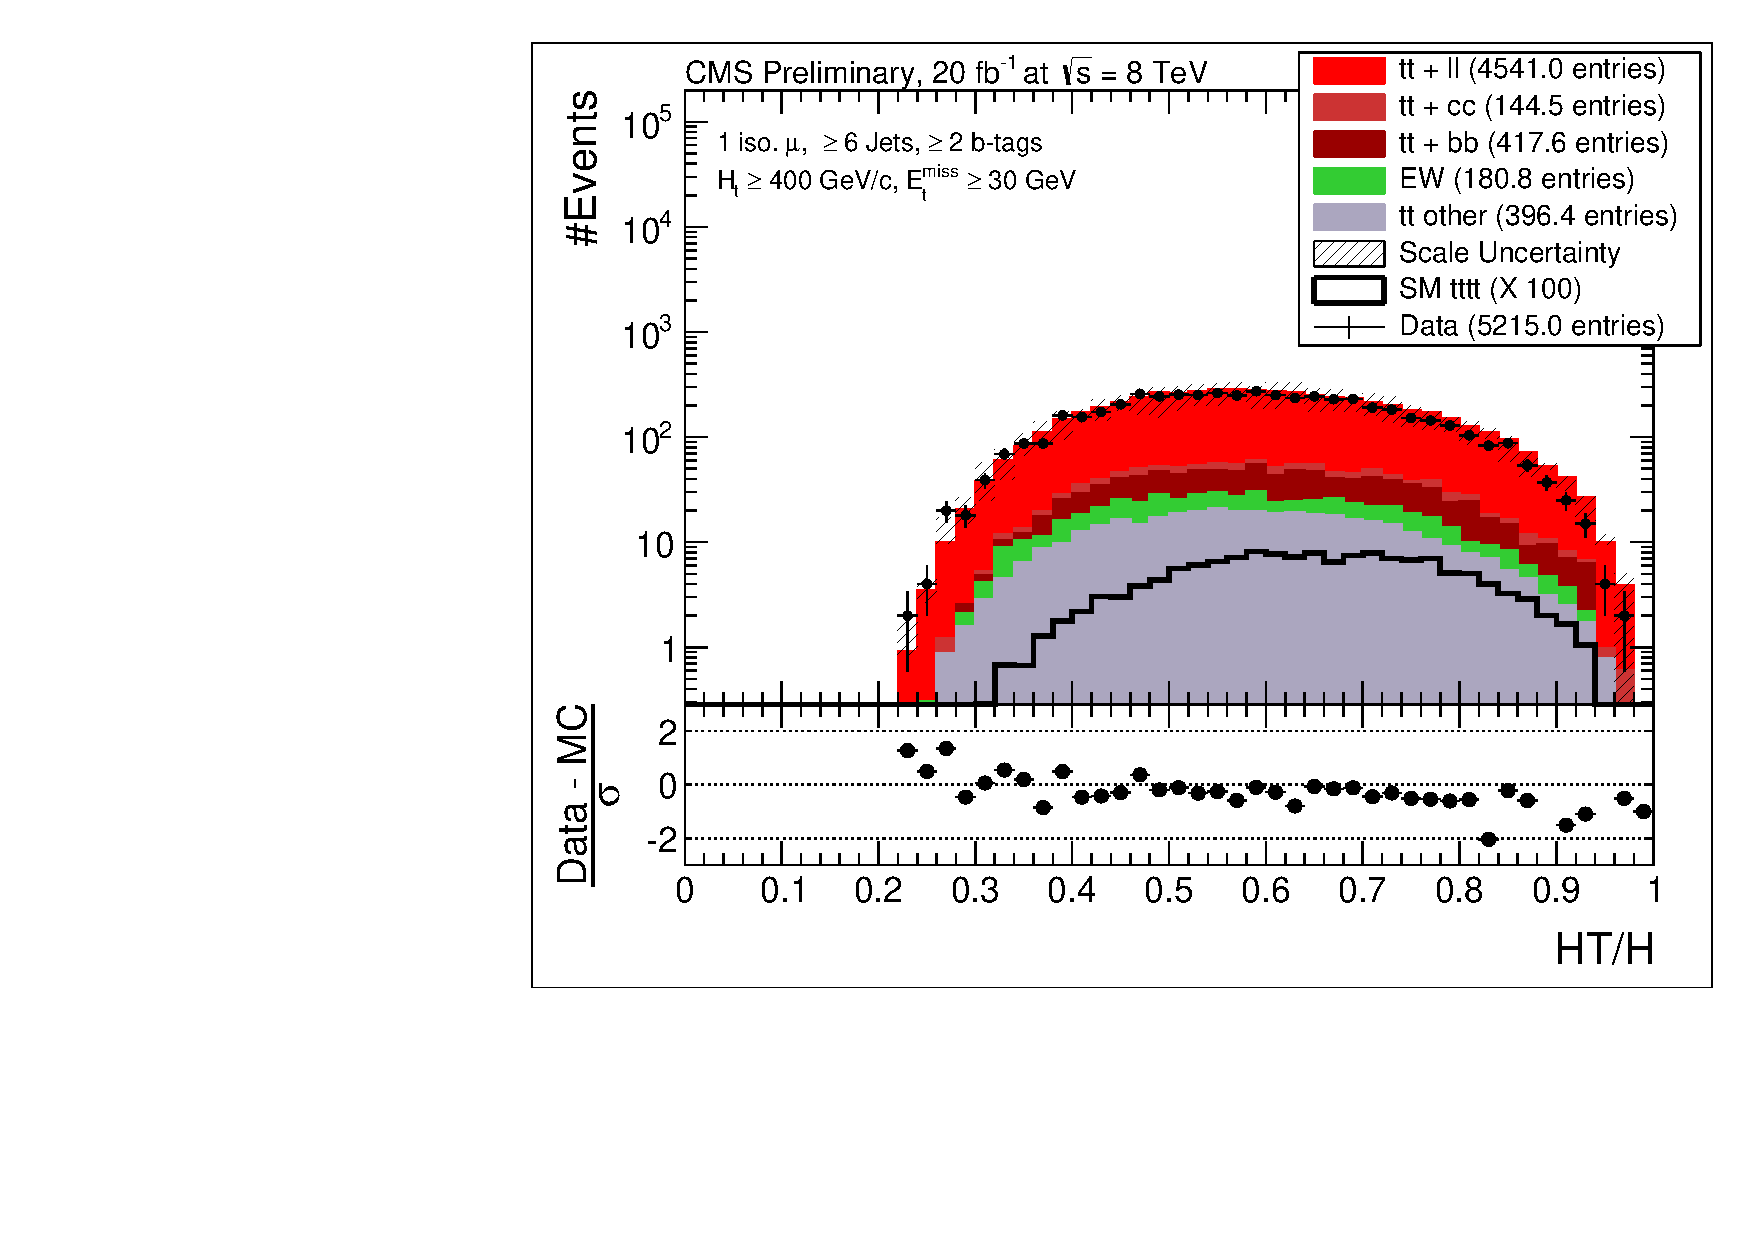
\includegraphics[width=0.49\textwidth]{images/Run1/HTH_StackLogY_Mu.pdf}
    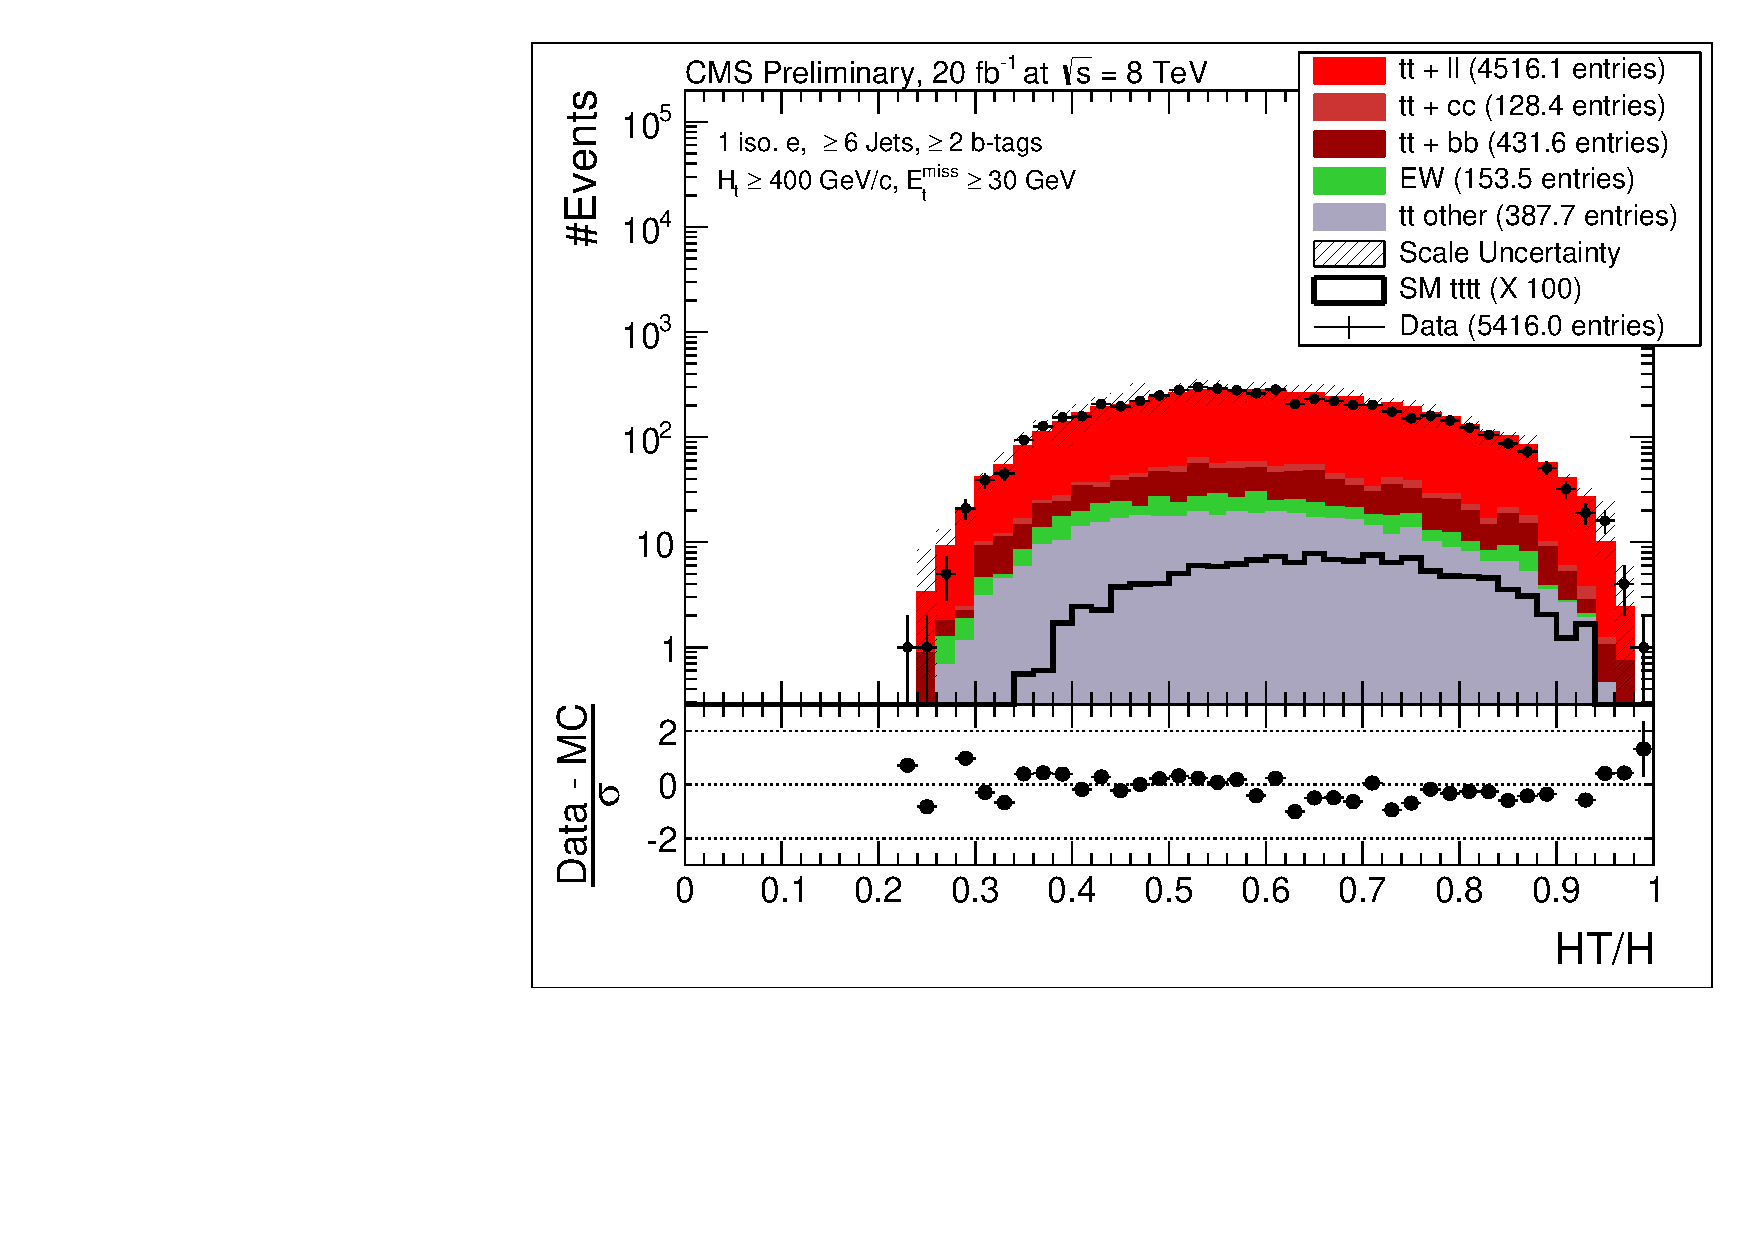
\includegraphics[width=0.49\textwidth]{images/Run1/HTH_StackLogY_e.pdf}
    \caption{Centrality for $\mu$ + jets (right) and e + jets (left).}
    \label{fig:HTrat}
\end{figure}

\begin{figure}[!ht]
    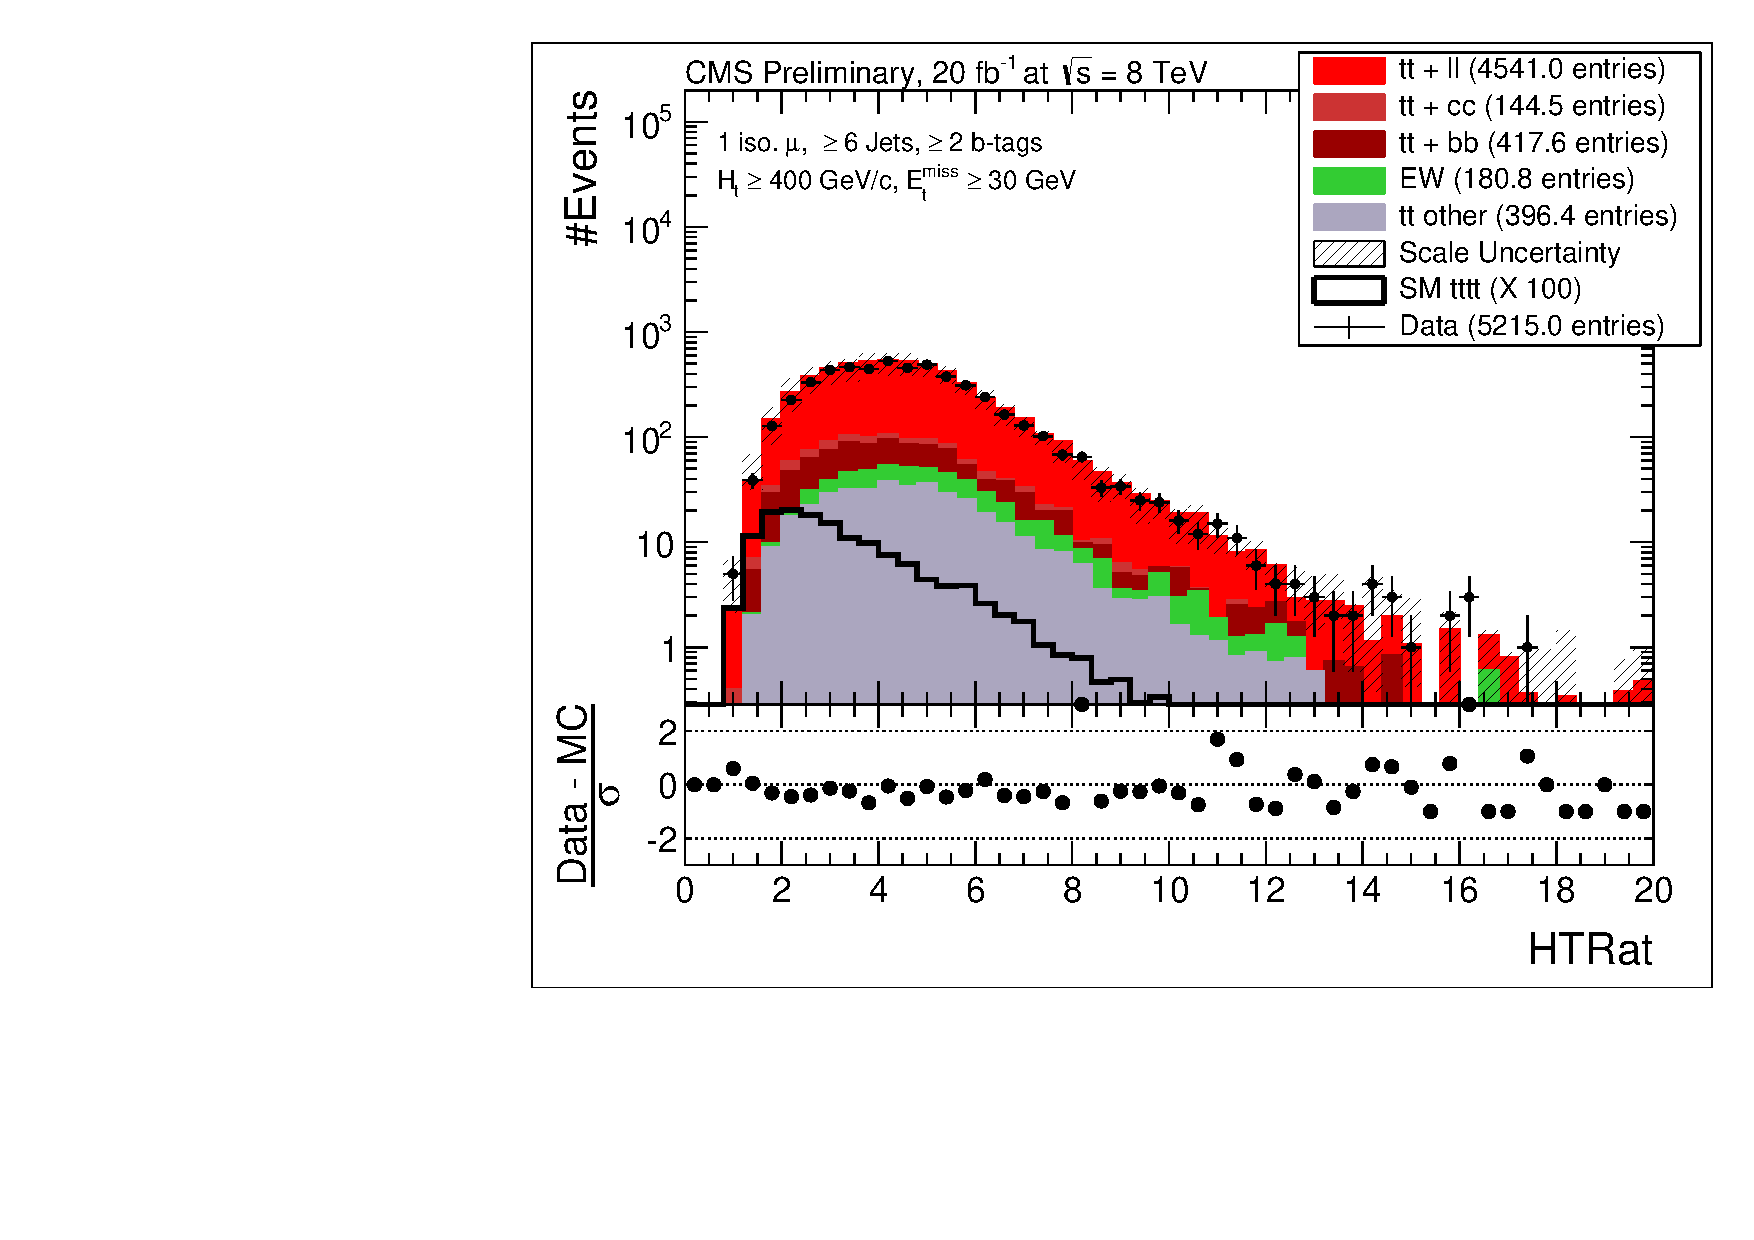
\includegraphics[width=0.49\textwidth]{images/Run1/HTRat_StackLogY_Mu.pdf}
    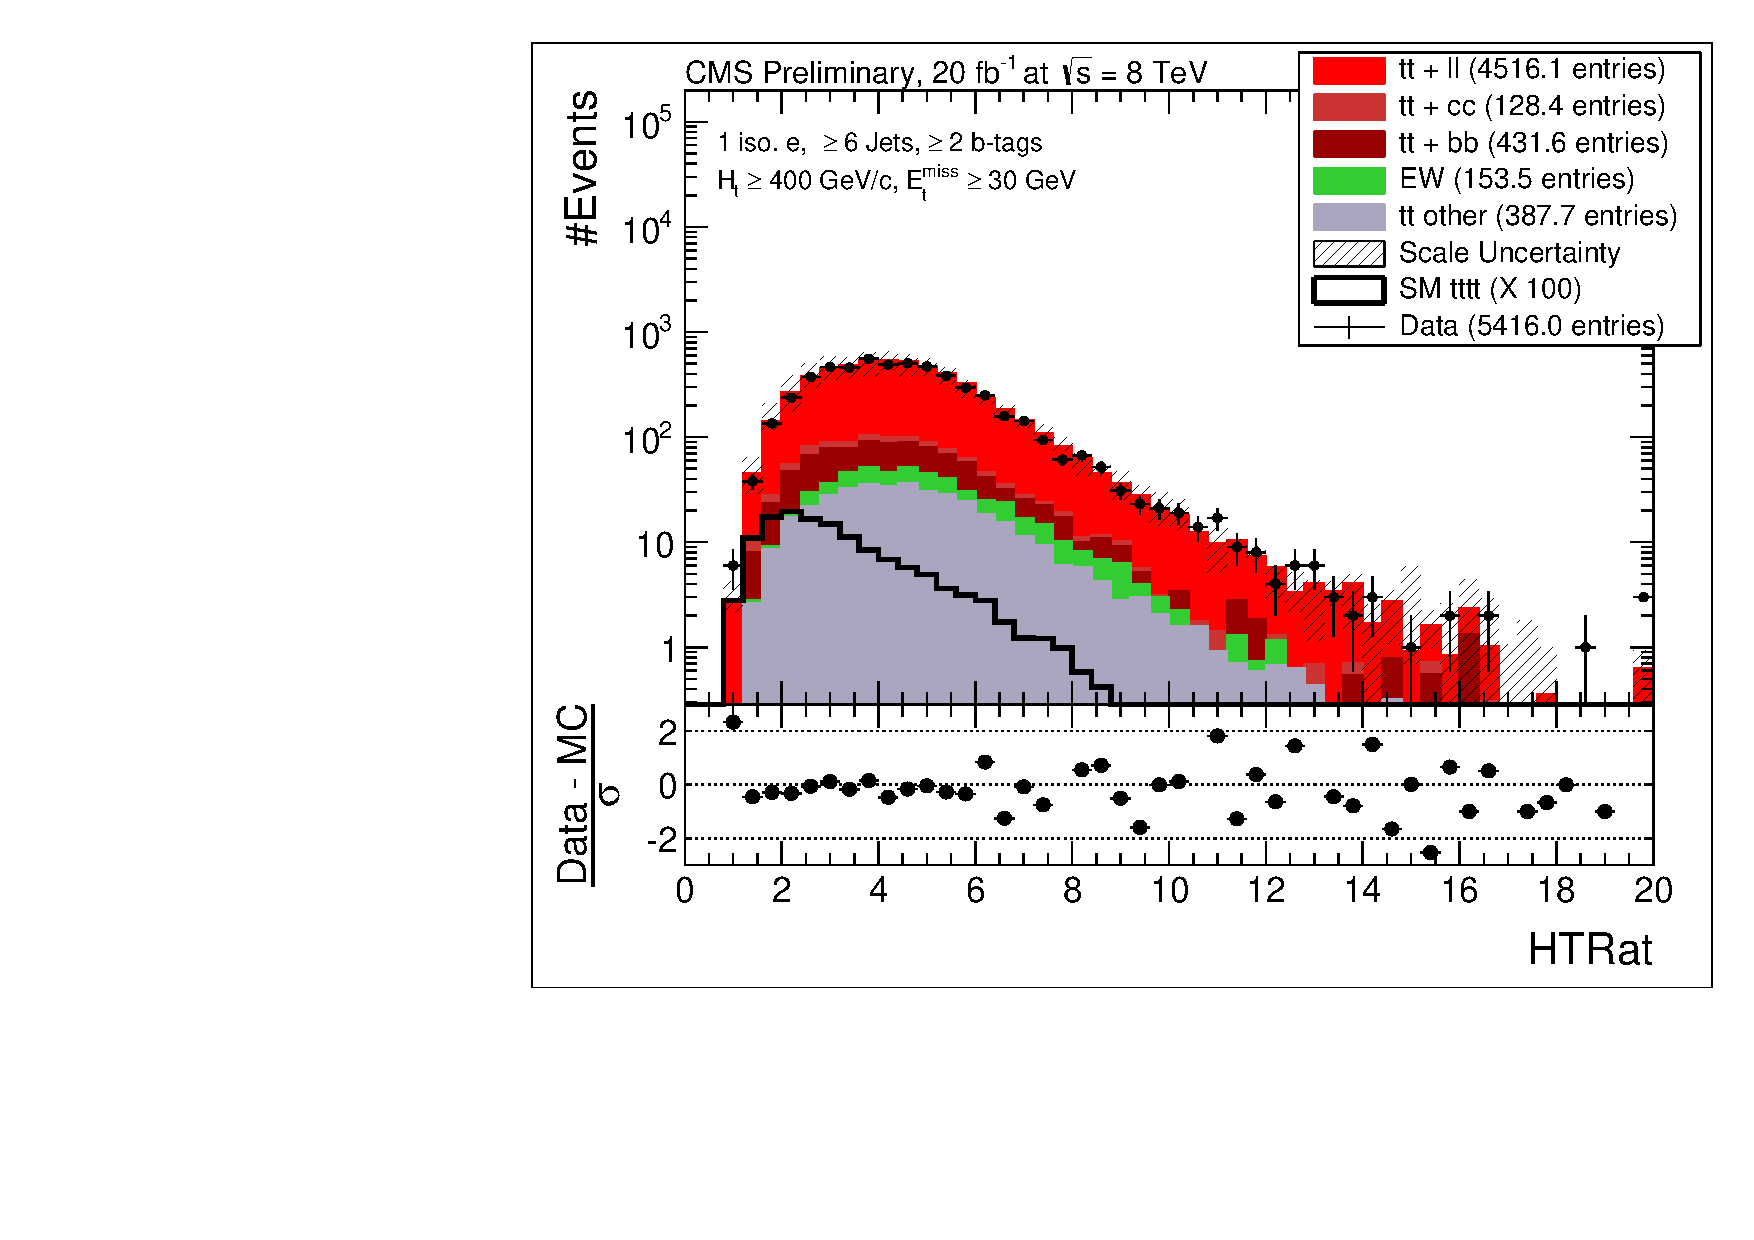
\includegraphics[width=0.49\textwidth]{images/Run1/HTRat_StackLogY_e.pdf}
    \caption{\HTrat for $\mu$ + jets (right) and e + jets (left).}
    \label{fig:HTrat}
\end{figure}

\begin{figure}[!ht]
    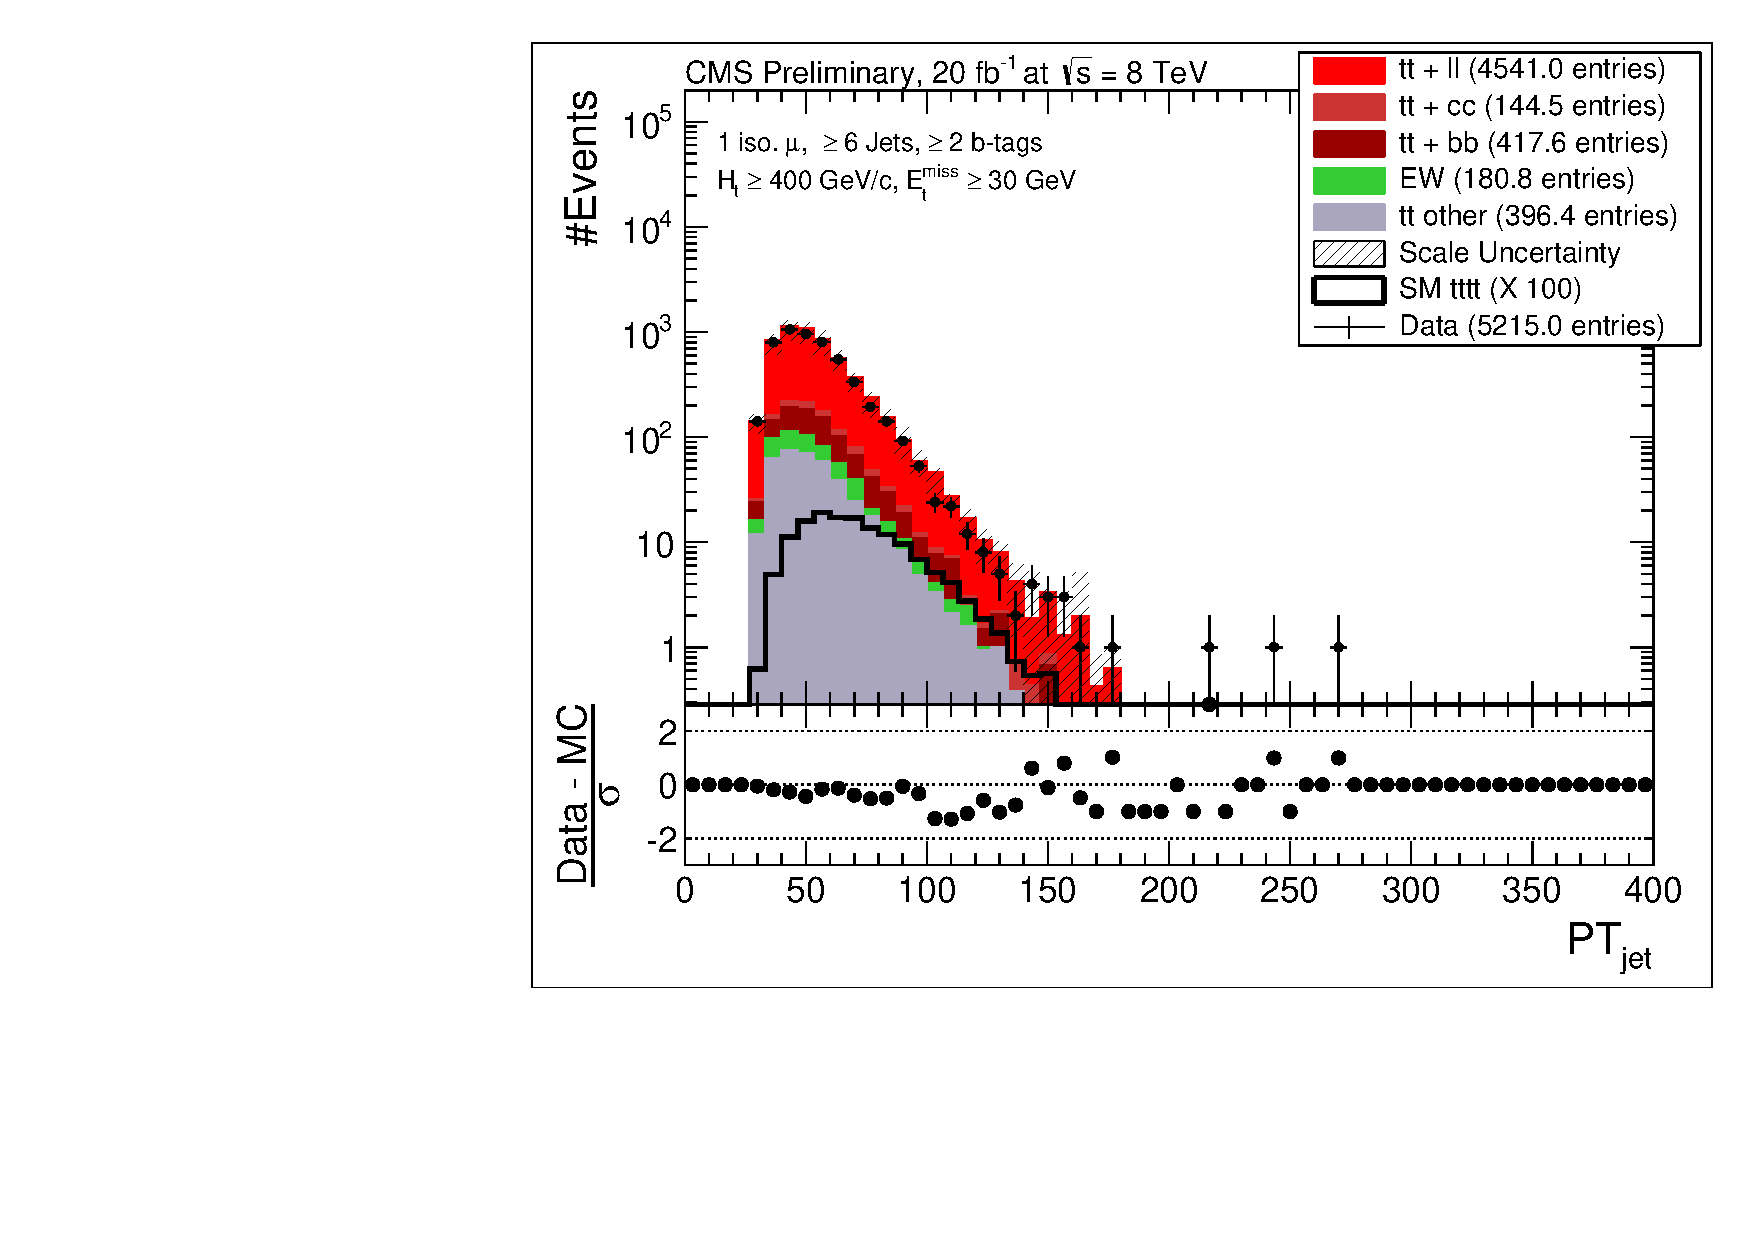
\includegraphics[width=0.49\textwidth]{images/Run1/5thJetPt_StackLogY_Mu.pdf}
    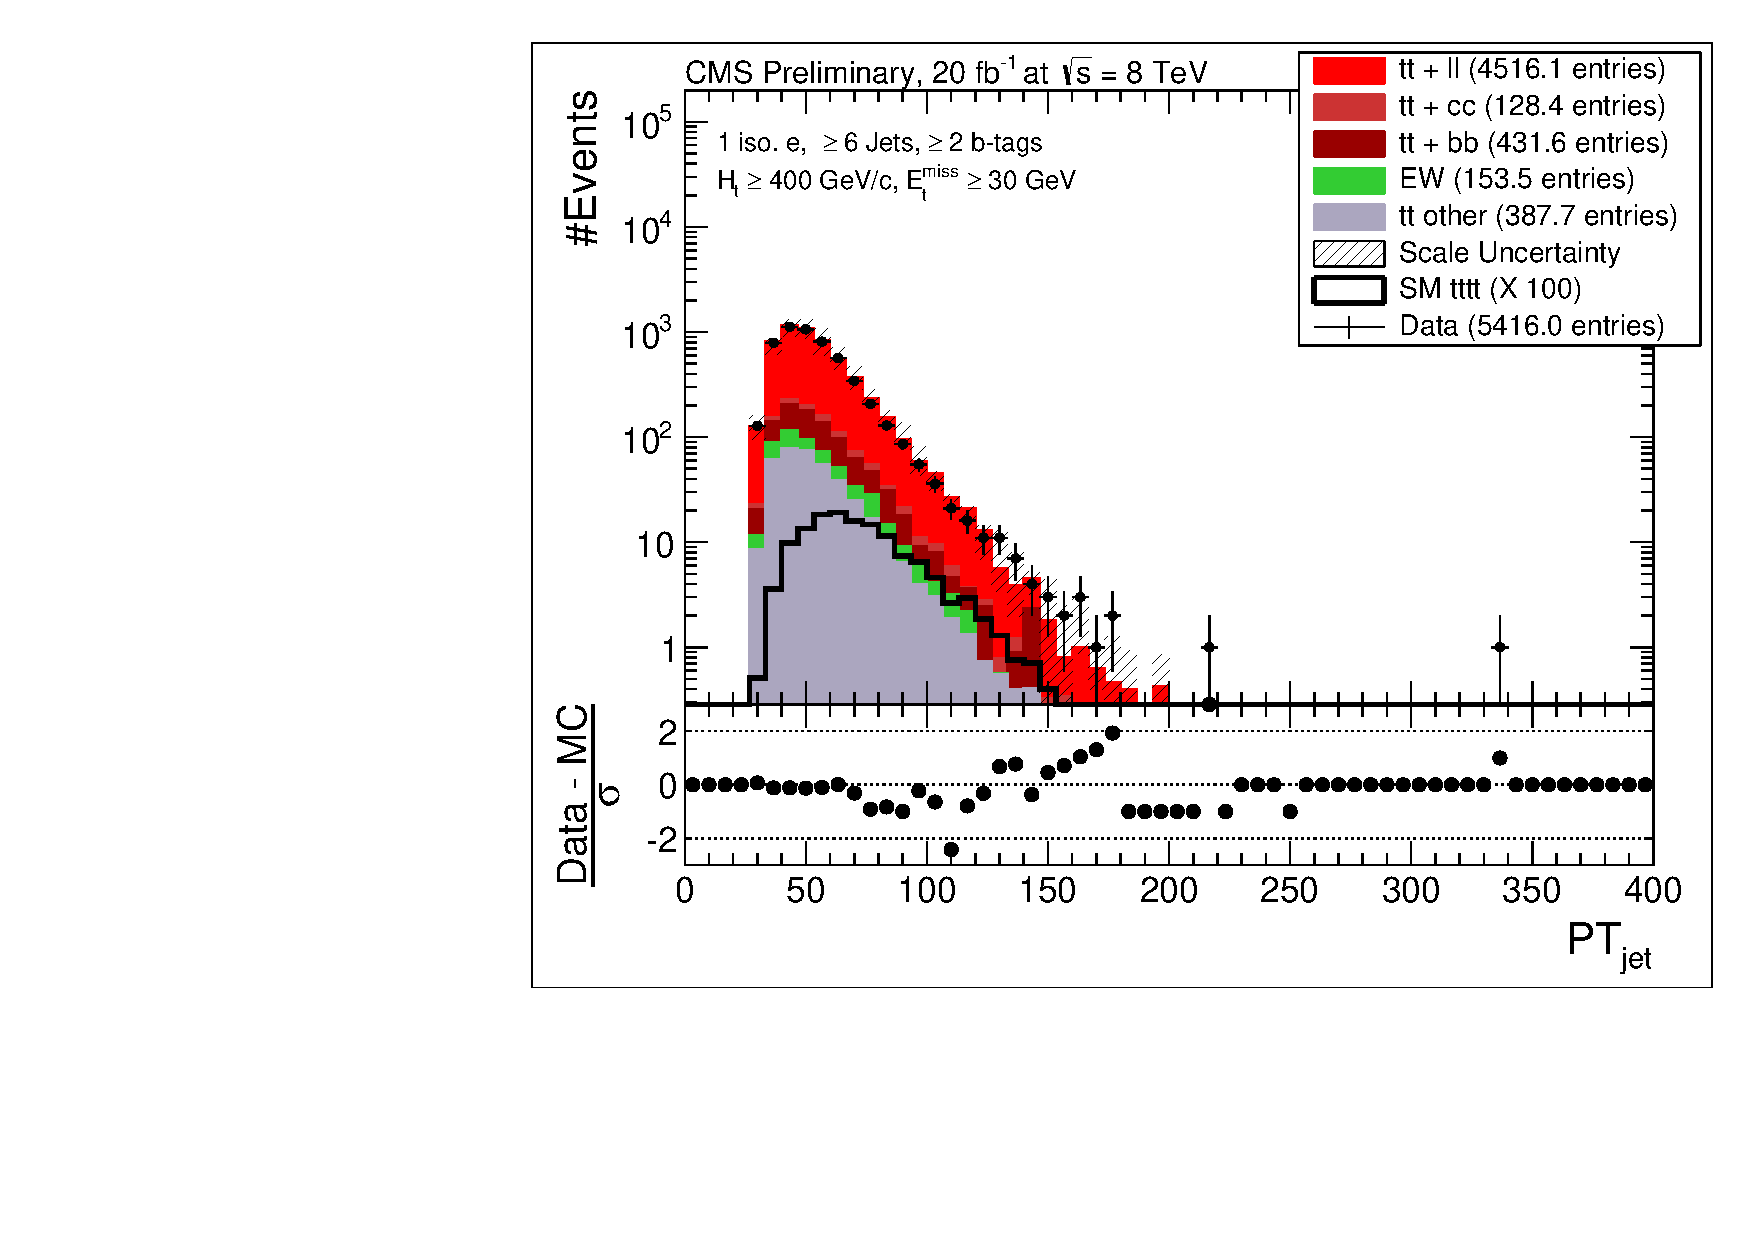
\includegraphics[width=0.49\textwidth]{images/Run1/5thJetPt_StackLogY_e.pdf}
    \caption{5th jet \pt for $\mu$ + jets (right) and e + jets (left).}
    \label{fig:5thjetpt}
\end{figure}

\begin{figure}[!ht]
    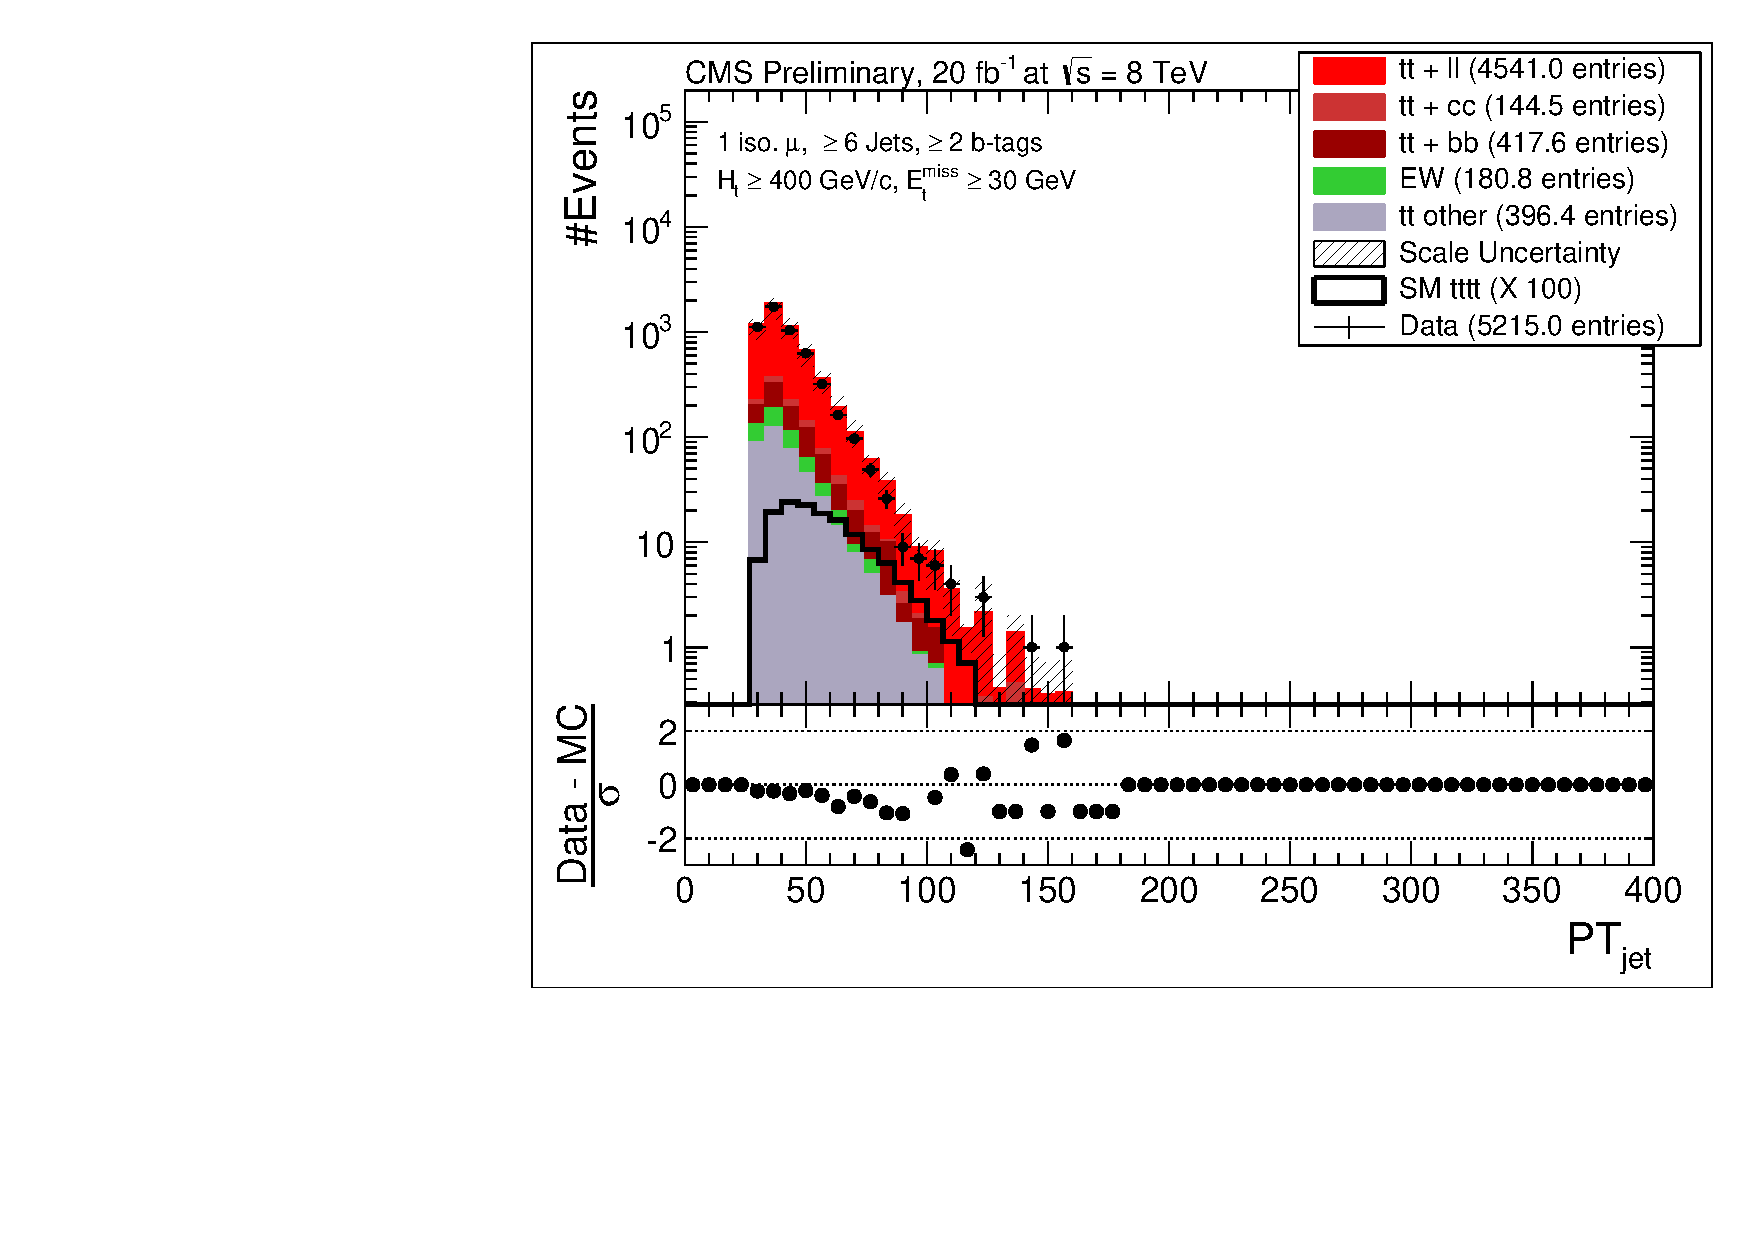
\includegraphics[width=0.49\textwidth]{images/Run1/6thJetPt_StackLogY_Mu.pdf}
    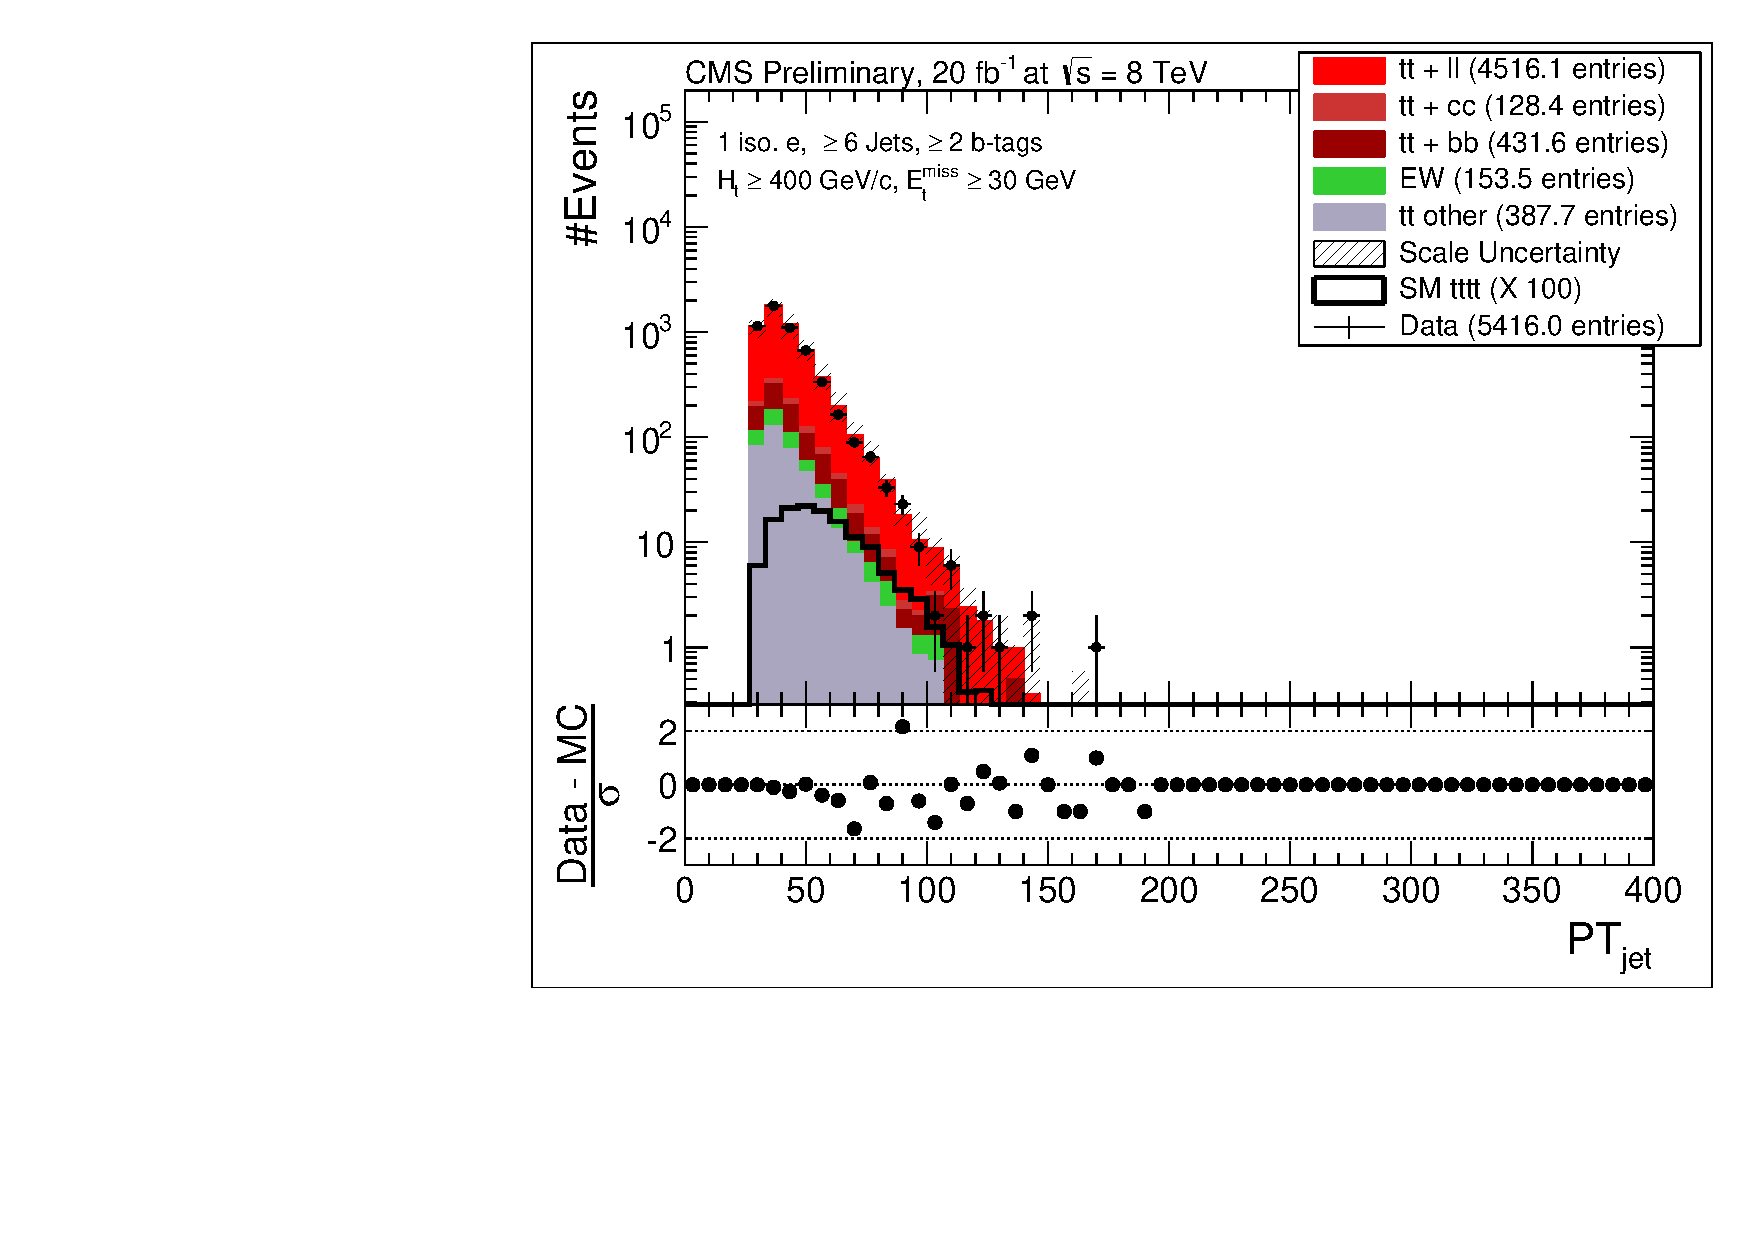
\includegraphics[width=0.49\textwidth]{images/Run1/6thJetPt_StackLogY_e.pdf}
    \caption{6th jet \pt for $\mu$ + jets (right) and e + jets (left).}
    \label{fig:6thjetpt}
\end{figure}

\subsection{Event-level BDT}
All of the variables described in Sections~\ref{sec:topContent},~\ref{sec:bottomContent} \&~\ref{sec:eventActivity} are used in a BDT, known as the event-level BDT. It is necessary to use a sample of events which were not used to train the kinematic reconstruction of top quarks to train the event-level BDT so that an orthogonal training sample can be provided. An additional set of events are used to test the performance of the BDT. The output distribution of the BDT discriminator can be seen in Fig.~\ref{fig:BDT}.

\begin{figure}[!ht]
    \includegraphics[width=0.49\textwidth]{images/Run1/MVA_Mu.pdf}
    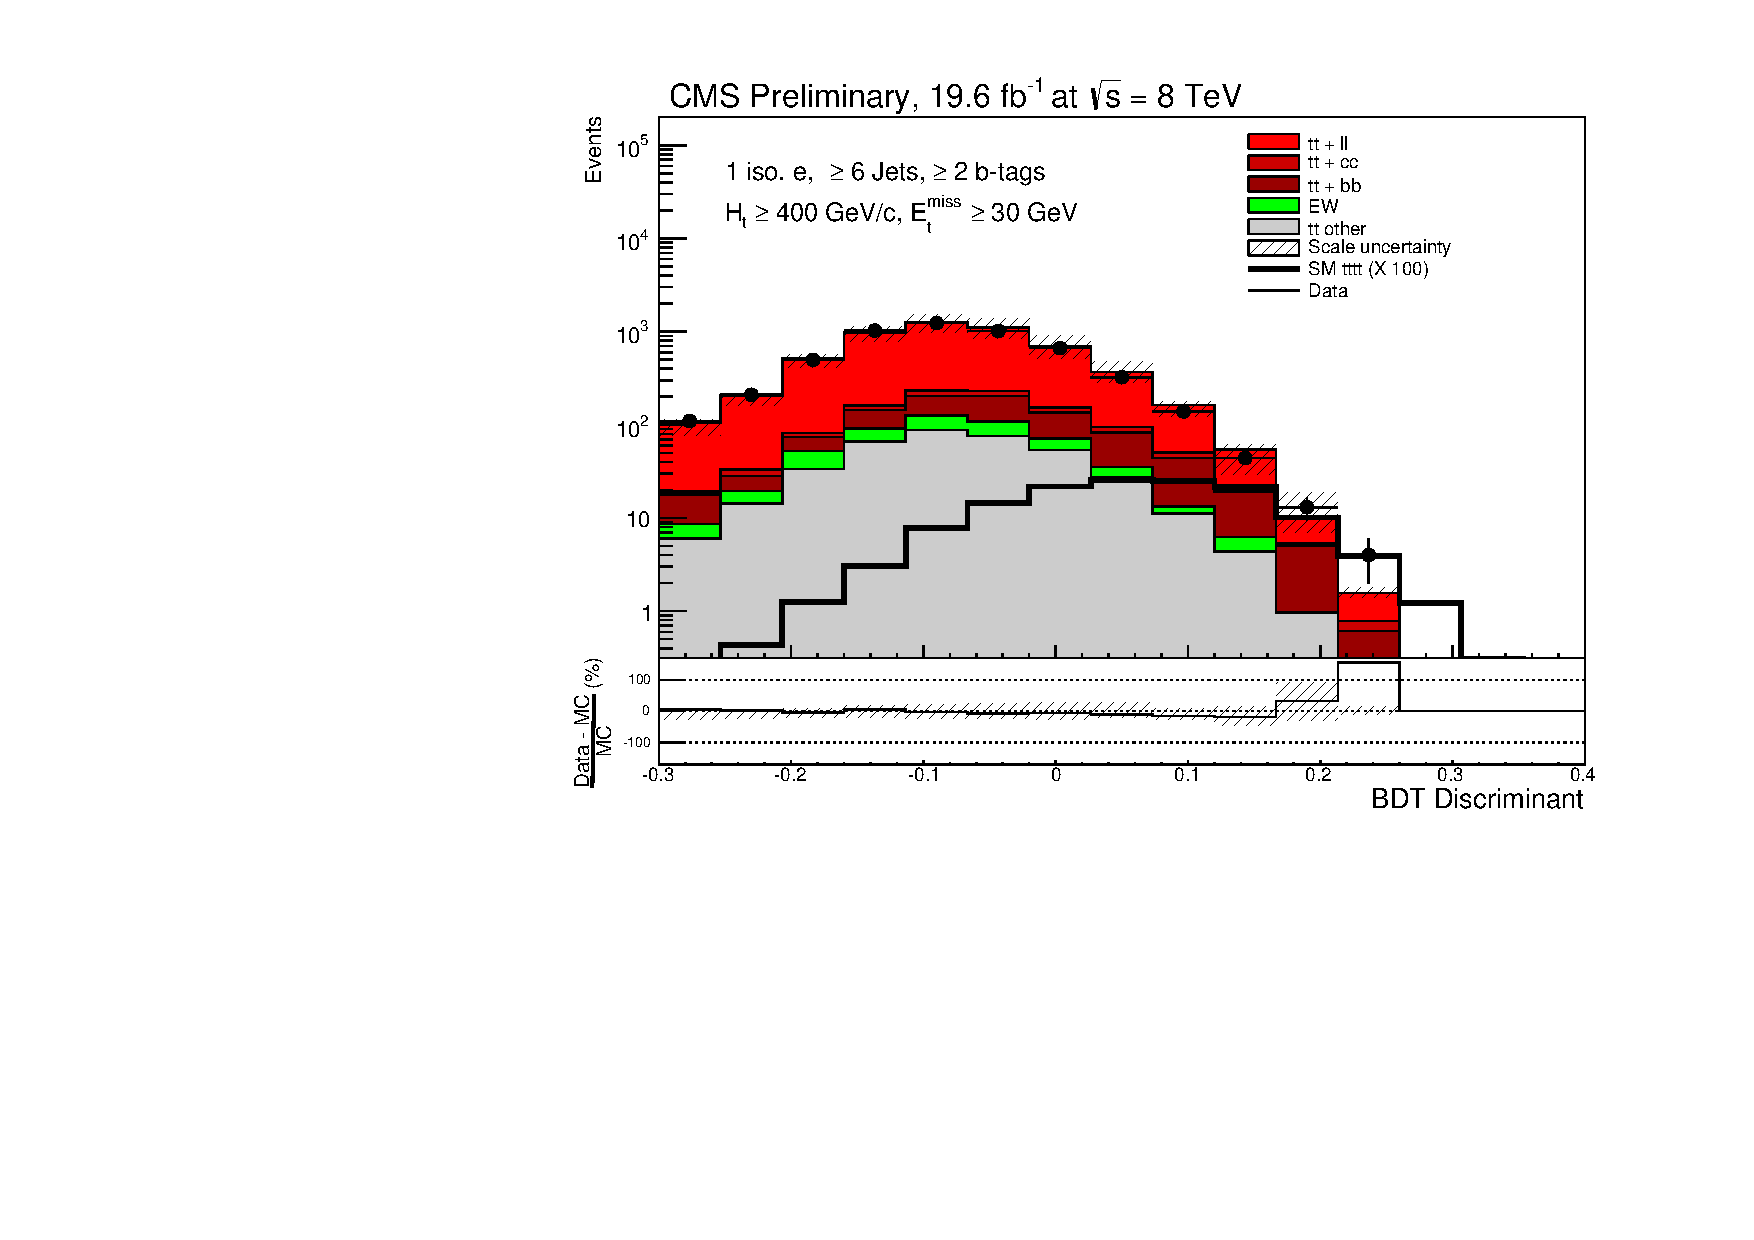
\includegraphics[width=0.49\textwidth]{images/Run1/MVA_e.pdf}
    \caption{BDT discriminator variable in data and simulation for $\mu$ + jets (right) and e + jets (left).}
    \label{fig:BDT}
\end{figure}

\section{Systematic uncertainties}
\label{sec:uncertainties}
There are two categories of systematic uncertainties; (i) Uncertainties which affect the normalisation of the distributions which are applied to signal and background and (ii) uncertainties which affect the shape of the distributions which are applied to the dominant background, in this case \ttbar. 
\subsection{Normalisation uncertainties}
%The normalisation uncertainties will only affect the uncertainty on the expected limit rather than the limit itself when it is used in the template fit and limit setting procedure described in Section~\ref{sec:limit}.
Normalisation uncertainties include the following:
\begin{itemize}
\item \textbf{Luminosity}
The CMS Luminosity Group give a recommendation of 2.6$\%$ uncertainty on the luminosity~\cite{CMS-PAS-LUM-12-001}.
\item \textbf{Monte Carlo cross sections}
As \ttbar is the main background to \tttt, the uncertainty on its MC cross-section is expected to be dominant over the other background processes. The uncertainty on \ttbar is ${}^{+2.5\%}_{-3.4\%} \left( \textrm{renormalisation and factorisation scale} \right)$ and ${}^{+2.5\%}_{-2.6\%} \left( \textrm{PDF} \right)$~\cite{PhysRevLett.110.252004}.
\fxnote*{??}{The MC cross section uncertainties are modelled by assigning a $4\%$ uncertainty to each background process and a $10\%$ uncertainty to the signal process}
\end{itemize}

\subsection{Shape uncertainties}
 Shape uncertainties arise from the following quantities.
 \fxnote{these quantities must be previously defined}
 \begin{itemize}
\item \textbf{Factorisation and renormalisation scales}
\item \textbf{Matching threshold}
\item \textbf{JES}
\item \textbf{JER}
\item \textbf{b tagging}
\item \textbf{Pile up}
\item \textbf{\heavyflavour modelling}
 \end{itemize}
 
The analysis procedure is repeated with \ttbar samples which have the respective quantity varied by $\pm 1 \sigma$ in order the produce new BDT templates with a deviated shape However, in the case of the matching threshold, the alternative shapes are produced by varying the matching threshold up to 40 GeV and down to 20 GeV.

\section{Template fit and upper limit}
\label{sec:limit}

An upper limit was calculated on the signal strength, \signalstrength , as no excess was observed in the data. Firstly, a template fit of the BDT distributions is made using the Combine Tool~\cite{CMS-NOTE-2011-005}, where the systematic uncertainties are modelled as nuisance parameters. Shape uncertainties are constrained using gaussian terms with exponential interpolation whereas the normalisation uncertainties are constrained using lognormal terms. For the statistical uncertainties, a lightweight version of the {Beeston and Barlow method~\cite{Conway:2011in} was used. This gives one nuisance parameter for the total MC estimate and a statistical uncertainty on each bin. The background processes are grouped into the following templates for the fit: `\ttbar' for semi-leptonic \ttbar, `electroweak' for W $+$ jets and Z $+$ jets, and `\ttbar\textunderscore other' for all other \ttbar processes. Using the \CLS method~\cite{Junk1999435,0954-3899-28-10-313} with the asymptotic approximation, the best fit values of the nuisance parameters can be obtained along with the corresponding limit on \signalstrength. The cross section limit, \sigmatttt, can be derived by multiplying the \signalstrength by \sigmattttSM $\approx 1.3$.

\subsection{Splitting into \njets categories}
\label{sec:njetcatlimit}
To increase the sensitivity of the analysis, the BDT templates were split into three \njets categories (\njets $= 6$, \njets $= 7 $ \& \njets $\geq 8$) each for the muon and electron channel. The higher \njets categories benefit from better discrimination power between signal and background as \tttt events are likely to have a larger number of jets. The \njets $= 6$ category helps to constrain the main background of \ttbar. A simultaneous fit of these three \njets categories is made for the muon channel, the electron channel and a combination of the two. The limits extracted using the \CLS method are shown in Table~\ref{tab:lims}.


\begin{table}[ht!]
\centering
\begin{tabular}{| l | l | l | p{1cm} |}
 \hline 
 Channel & Exp.  &Obs. \\
   \hline
 $\mu$ + jets & $35.6\pm 18$ & 34 \\
  \hline
$e$ + jets &  $36.1\pm16$  & 36  \\
\hline
 combined & $24.6\pm13$  & 25   \\
\hline
\end{tabular}
\hspace{0.5cm}
\begin{tabular}{| l | l | l | p{1cm} |}
 \hline 
 Channel & Exp. (fb) &Obs. (fb) \\
   \hline
 $\mu$ + jets & $46.3\pm23$ & 44 \\
  \hline
$e$ + jets &  $47.0\pm20$  & 47  \\
\hline
 combined & $32.0\pm17$  & 32   \\
\hline
\end{tabular}
\caption{CLS limits on (\sigmatttt/(\sigmattttSM) (left) and \sigmatttt (right). }
\label{tab:lims}
\end{table}

In comparison, the corresponding limit in a \fxnote*{ref PAS}{preliminary result} for a simultaneous fit of the electron and muon channels in inclusive \njets categories was observed to be 63 fb with an expected limit of  $42^{+18}_{-13}$ fb. Therefore, it can be seen that splitting into \njets categories provides a significant improvement in the sensitivity of the analysis.


\section{Signal Injection Test}
\label{sec:signalinjection}
In order to validate the limit-setting method, the following closure test was performed. A range of signal strengths were injected into the data and the limit-setting procedure was repeated as in Section~\ref{sec:limit}. Figure~\ref{fig:SigInjection} shows the BDT discriminator distributions with injected signal strengths of 20fb, 40fb and 60fb. With the increasing signal strength, there is an increase in the bins with a higher BDT discriminator values as would be expected for signal events.
\begin{figure}[ht!]
\centering
    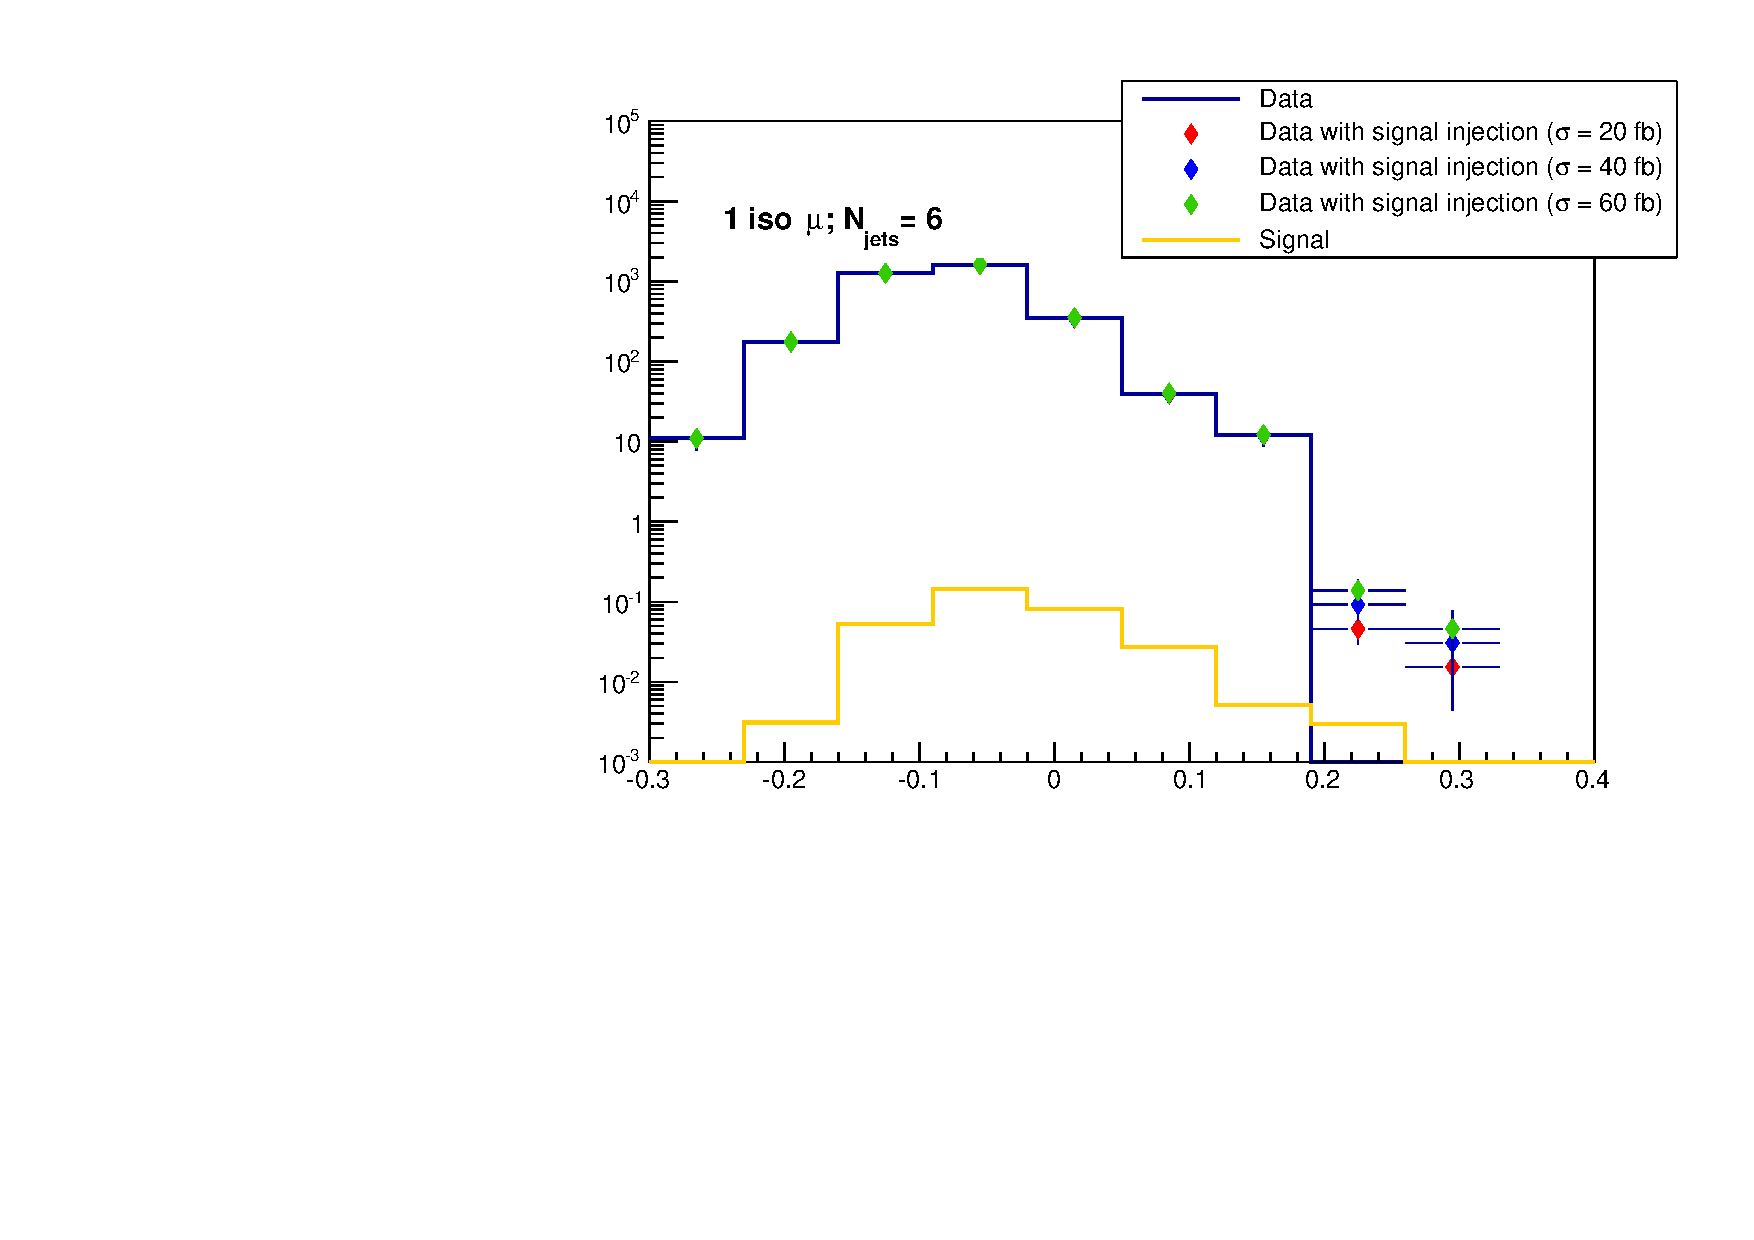
\includegraphics[width=0.49\textwidth]{images/Run1/SignalInjection_Mu_6j.pdf}
     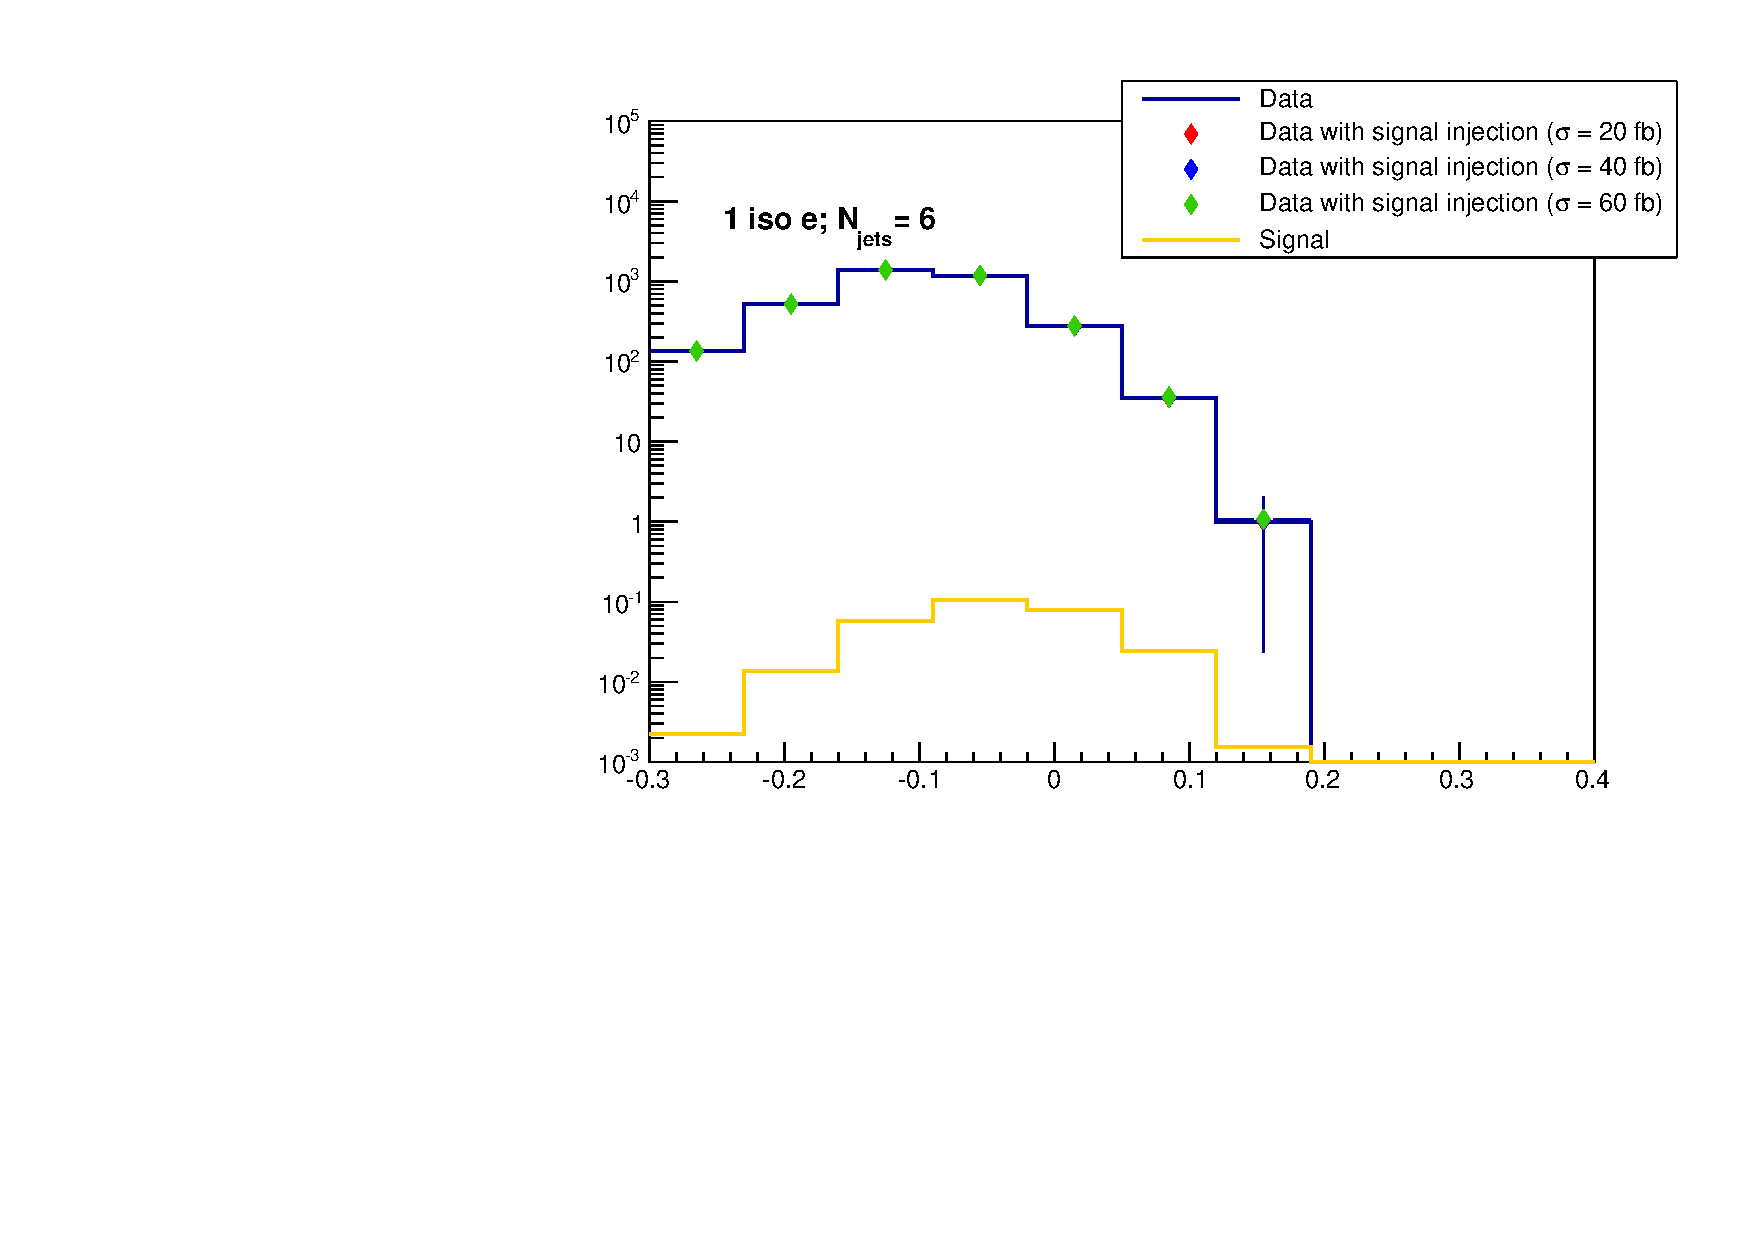
\includegraphics[width=0.49\textwidth]{images/Run1/SignalInjection_El_6j.pdf}
    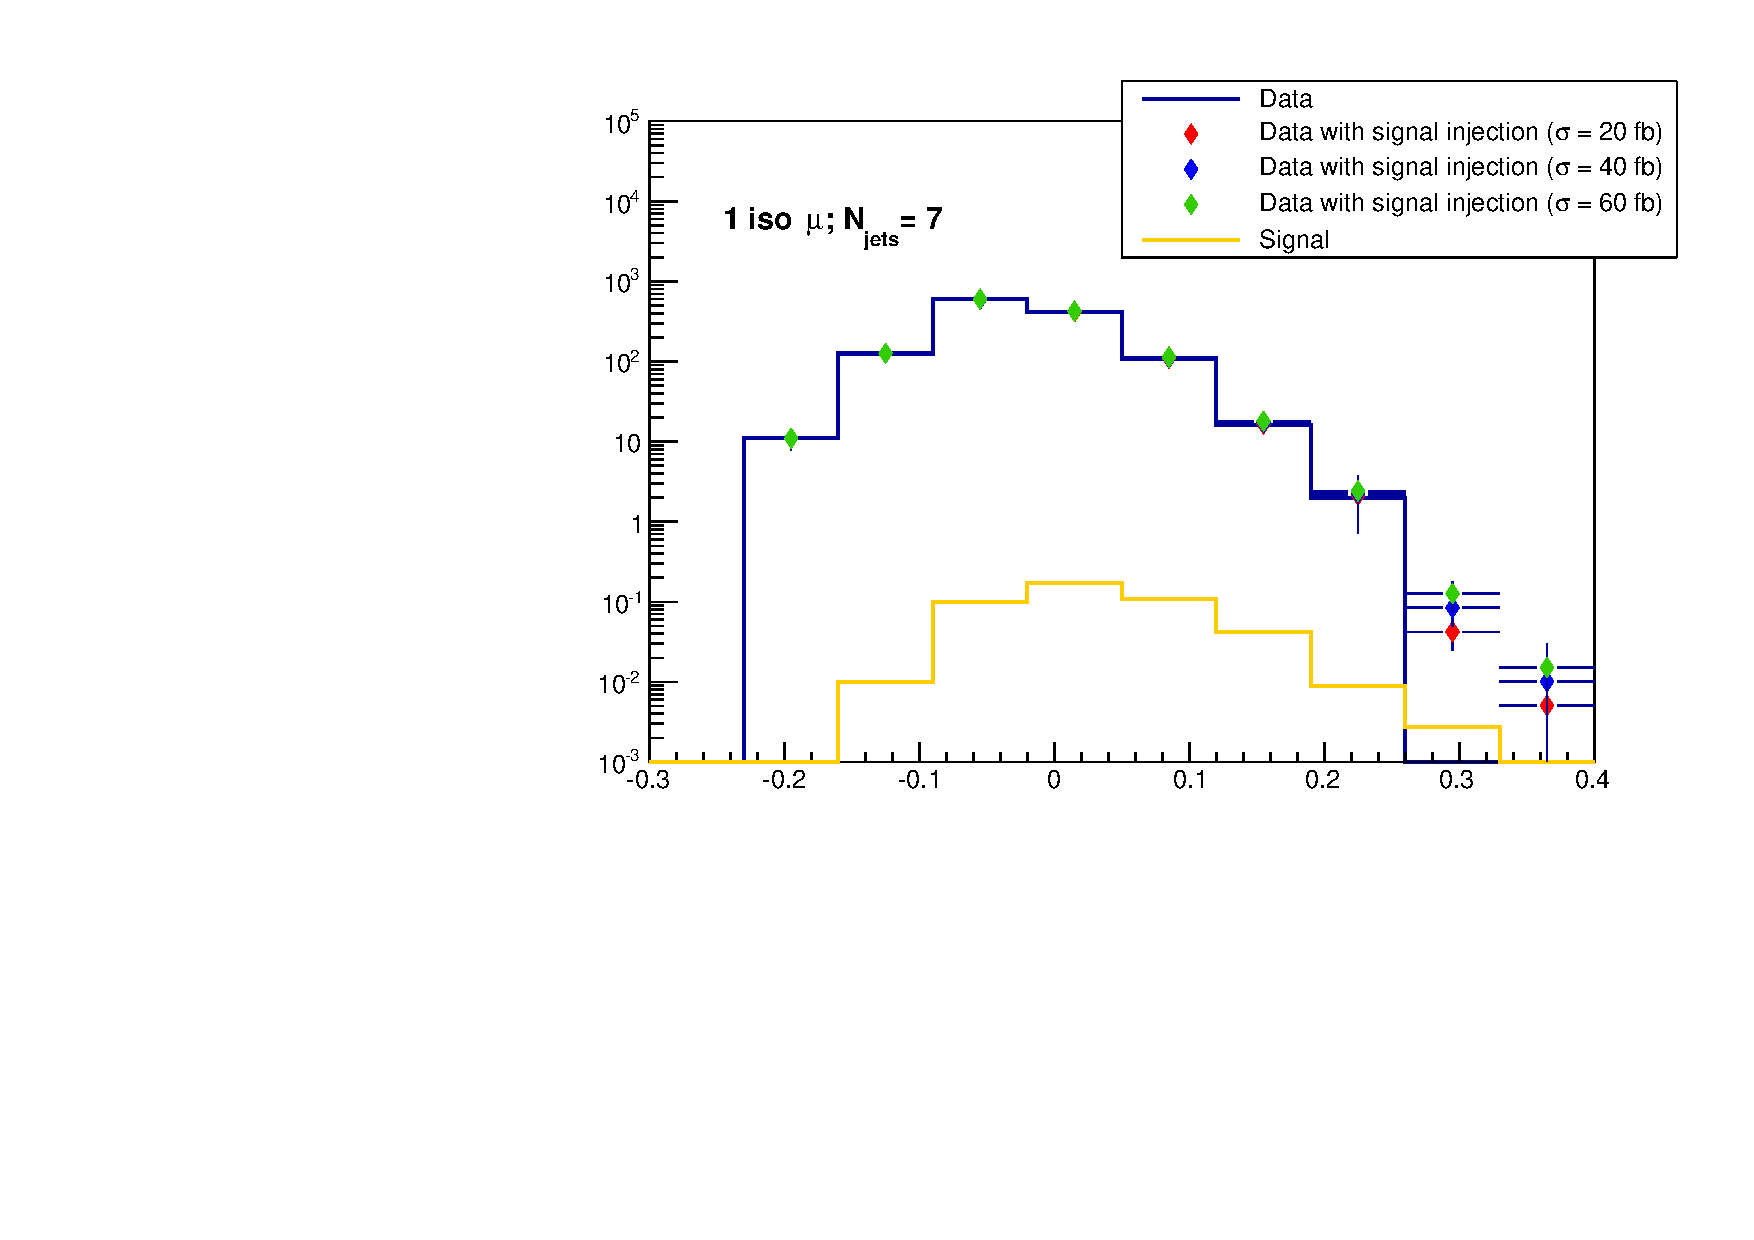
\includegraphics[width=0.49\textwidth]{images/Run1/SignalInjection_Mu_7j.pdf}
     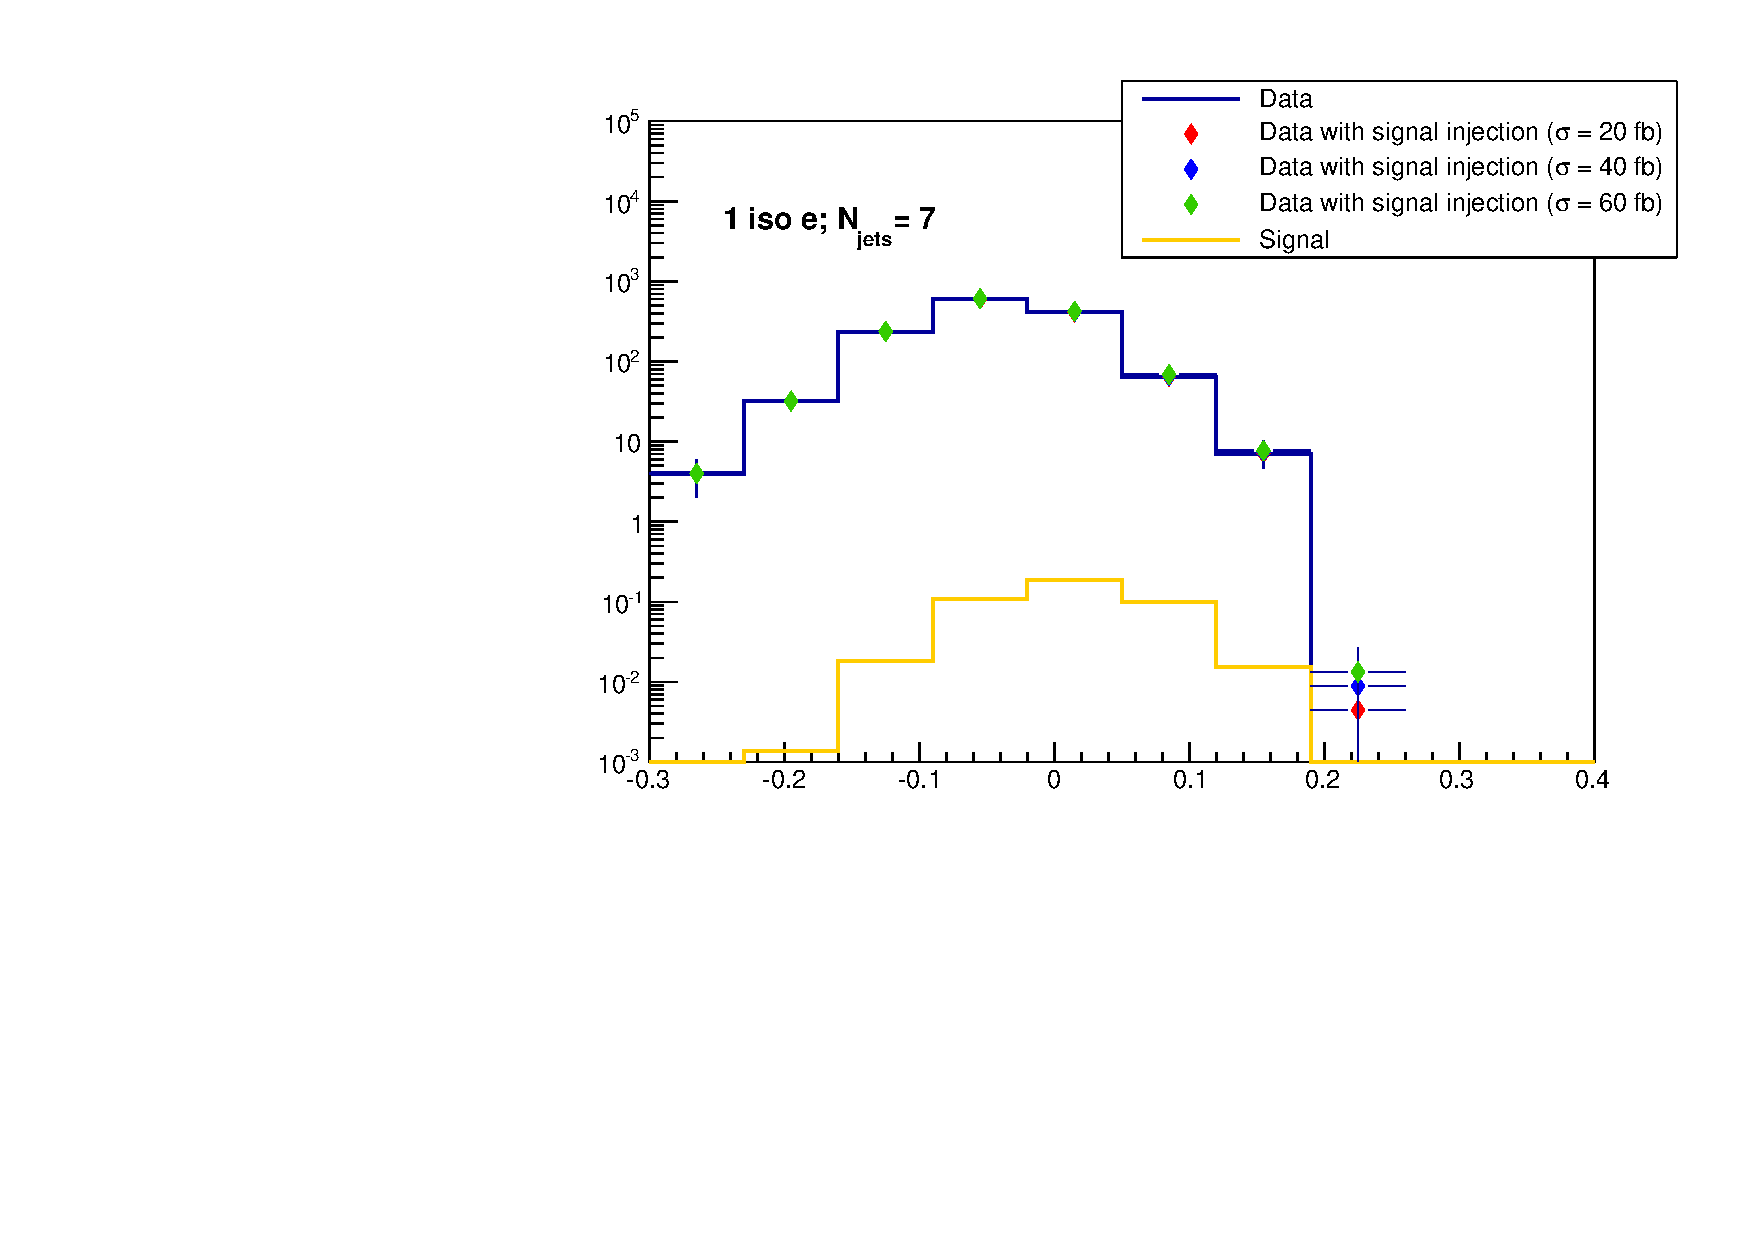
\includegraphics[width=0.49\textwidth]{images/Run1/SignalInjection_El_7j.pdf}
    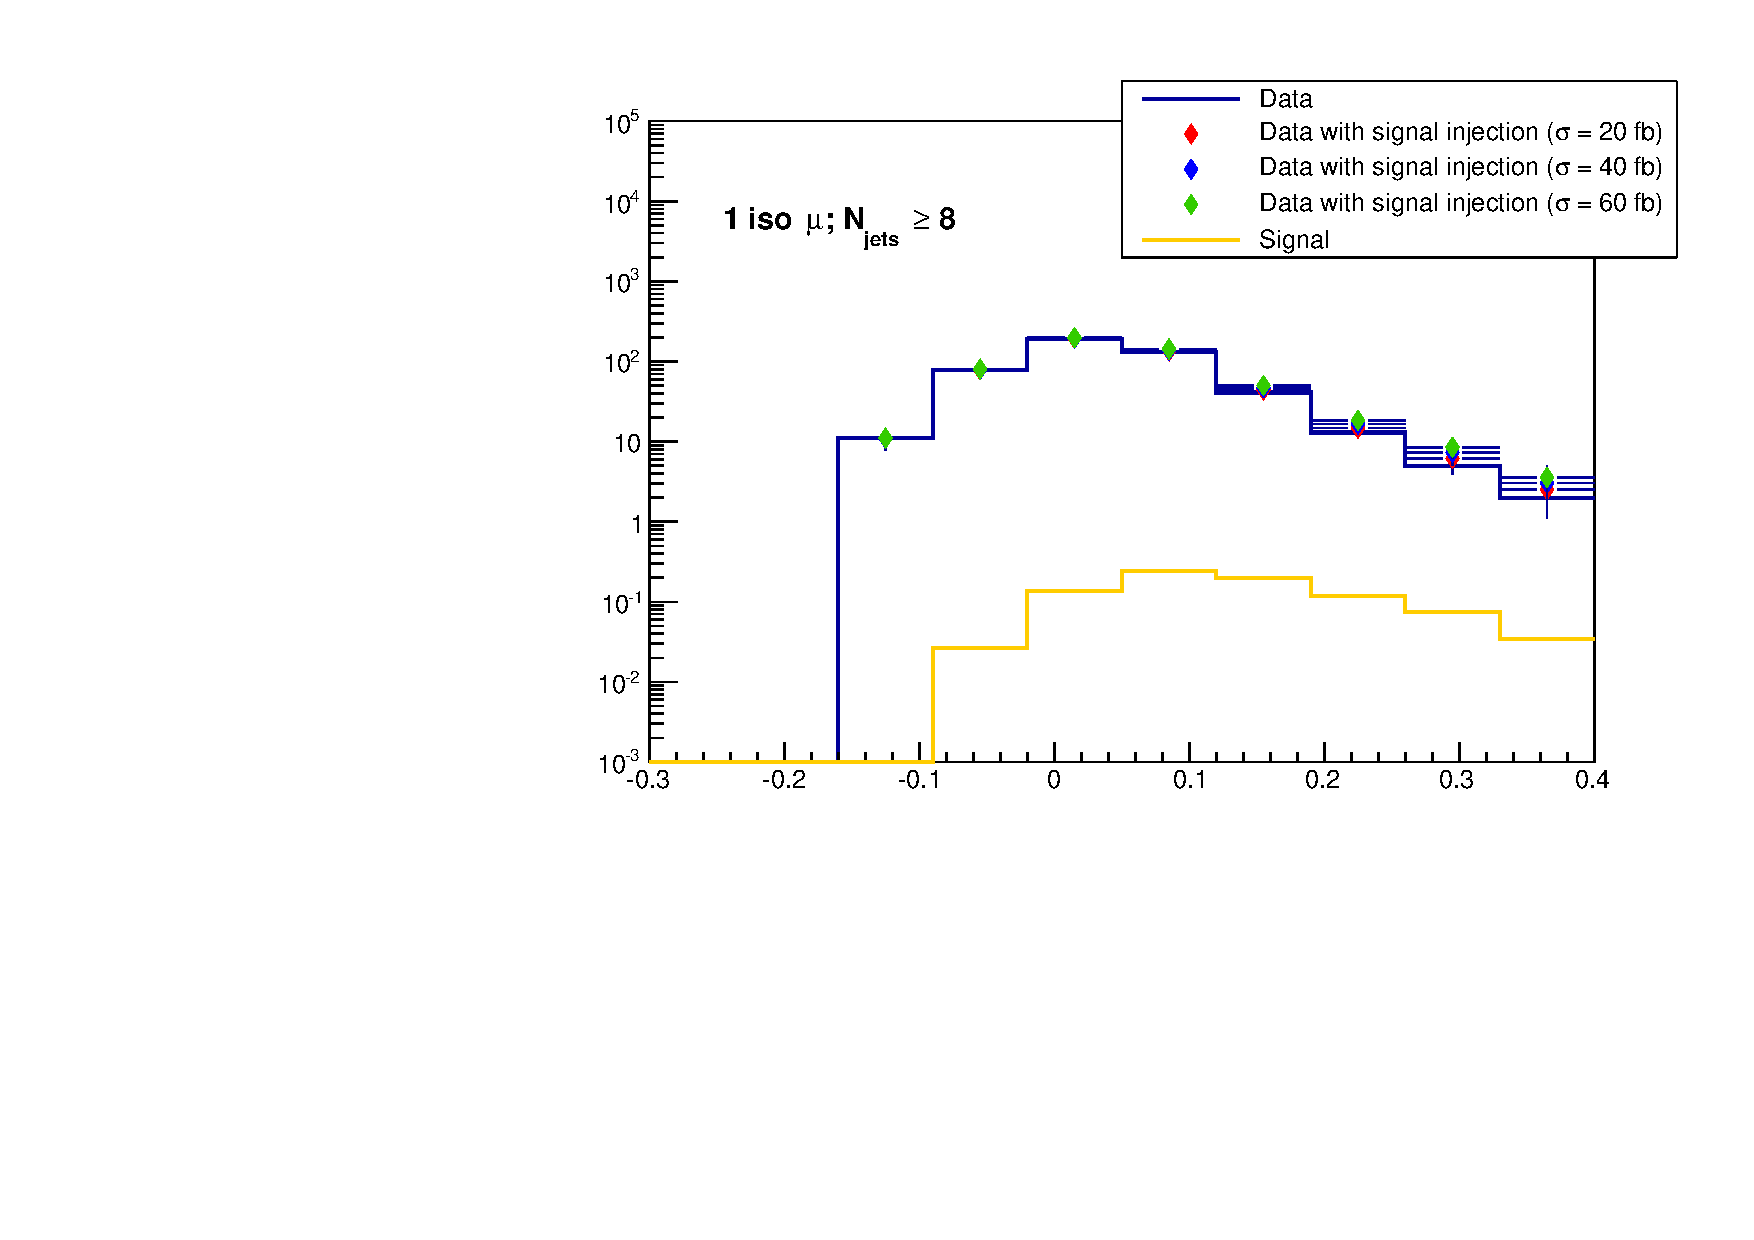
\includegraphics[width=0.49\textwidth]{images/Run1/SignalInjection_Mu_8j.pdf}
     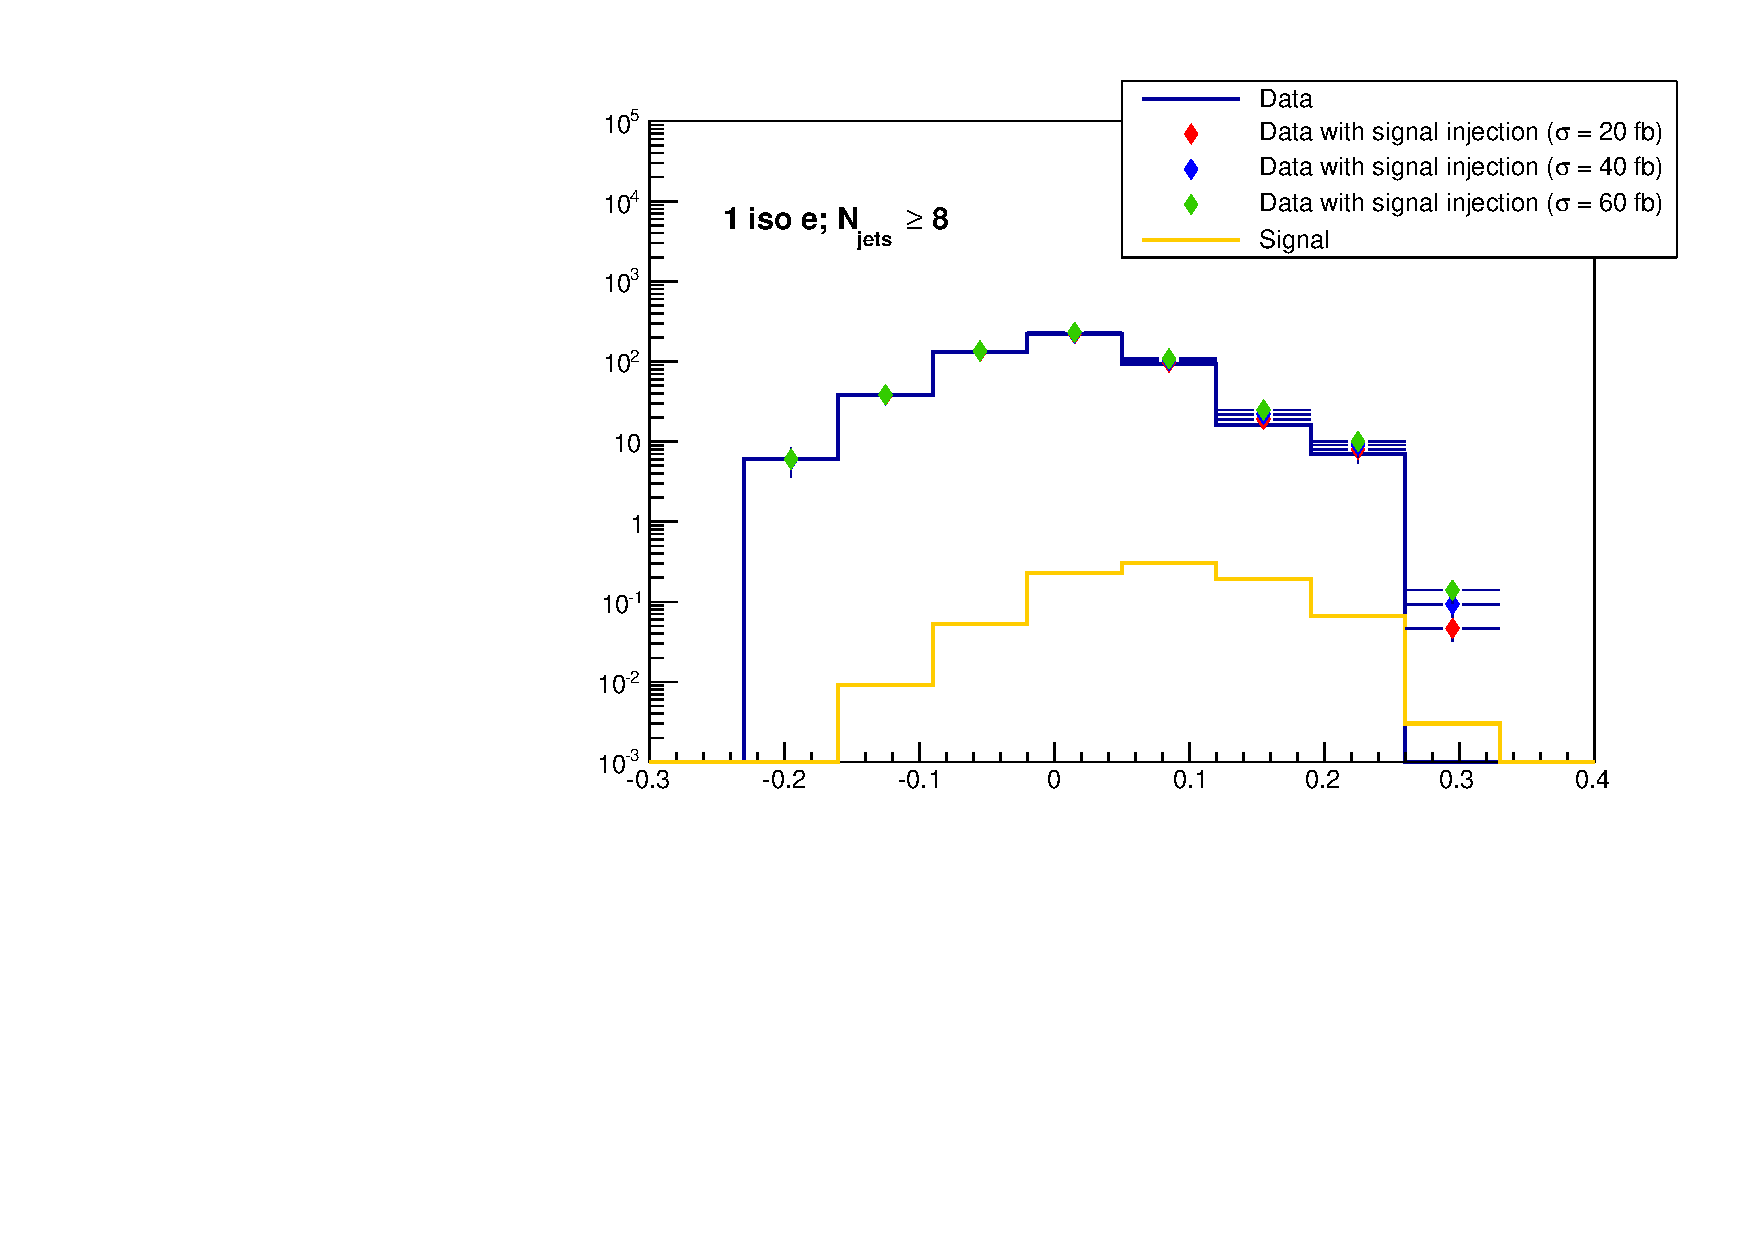
\includegraphics[width=0.49\textwidth]{images/Run1/SignalInjection_El_8j.pdf}          
    \caption{The BDT discriminator distributions of data and the mixtures of data and injected signal are compared for $\mu$ + jets channel $\left( \textrm{left} \right)$ and e + jets channel $\left( \textrm{right} \right)$. }
    \label{fig:SigInjection}
\end{figure}
As can be seen in Fig.~\ref{fig:SigInjectionBrazil}, the fitted value for the signal strength and observed limit increase with increasing injected singal strength as expected. However, there appears to be some bias in the analysis towards selecting background as opposed to signal as can be seen from the gradient of the line, which is $<$1.
\begin{figure}[!ht]
    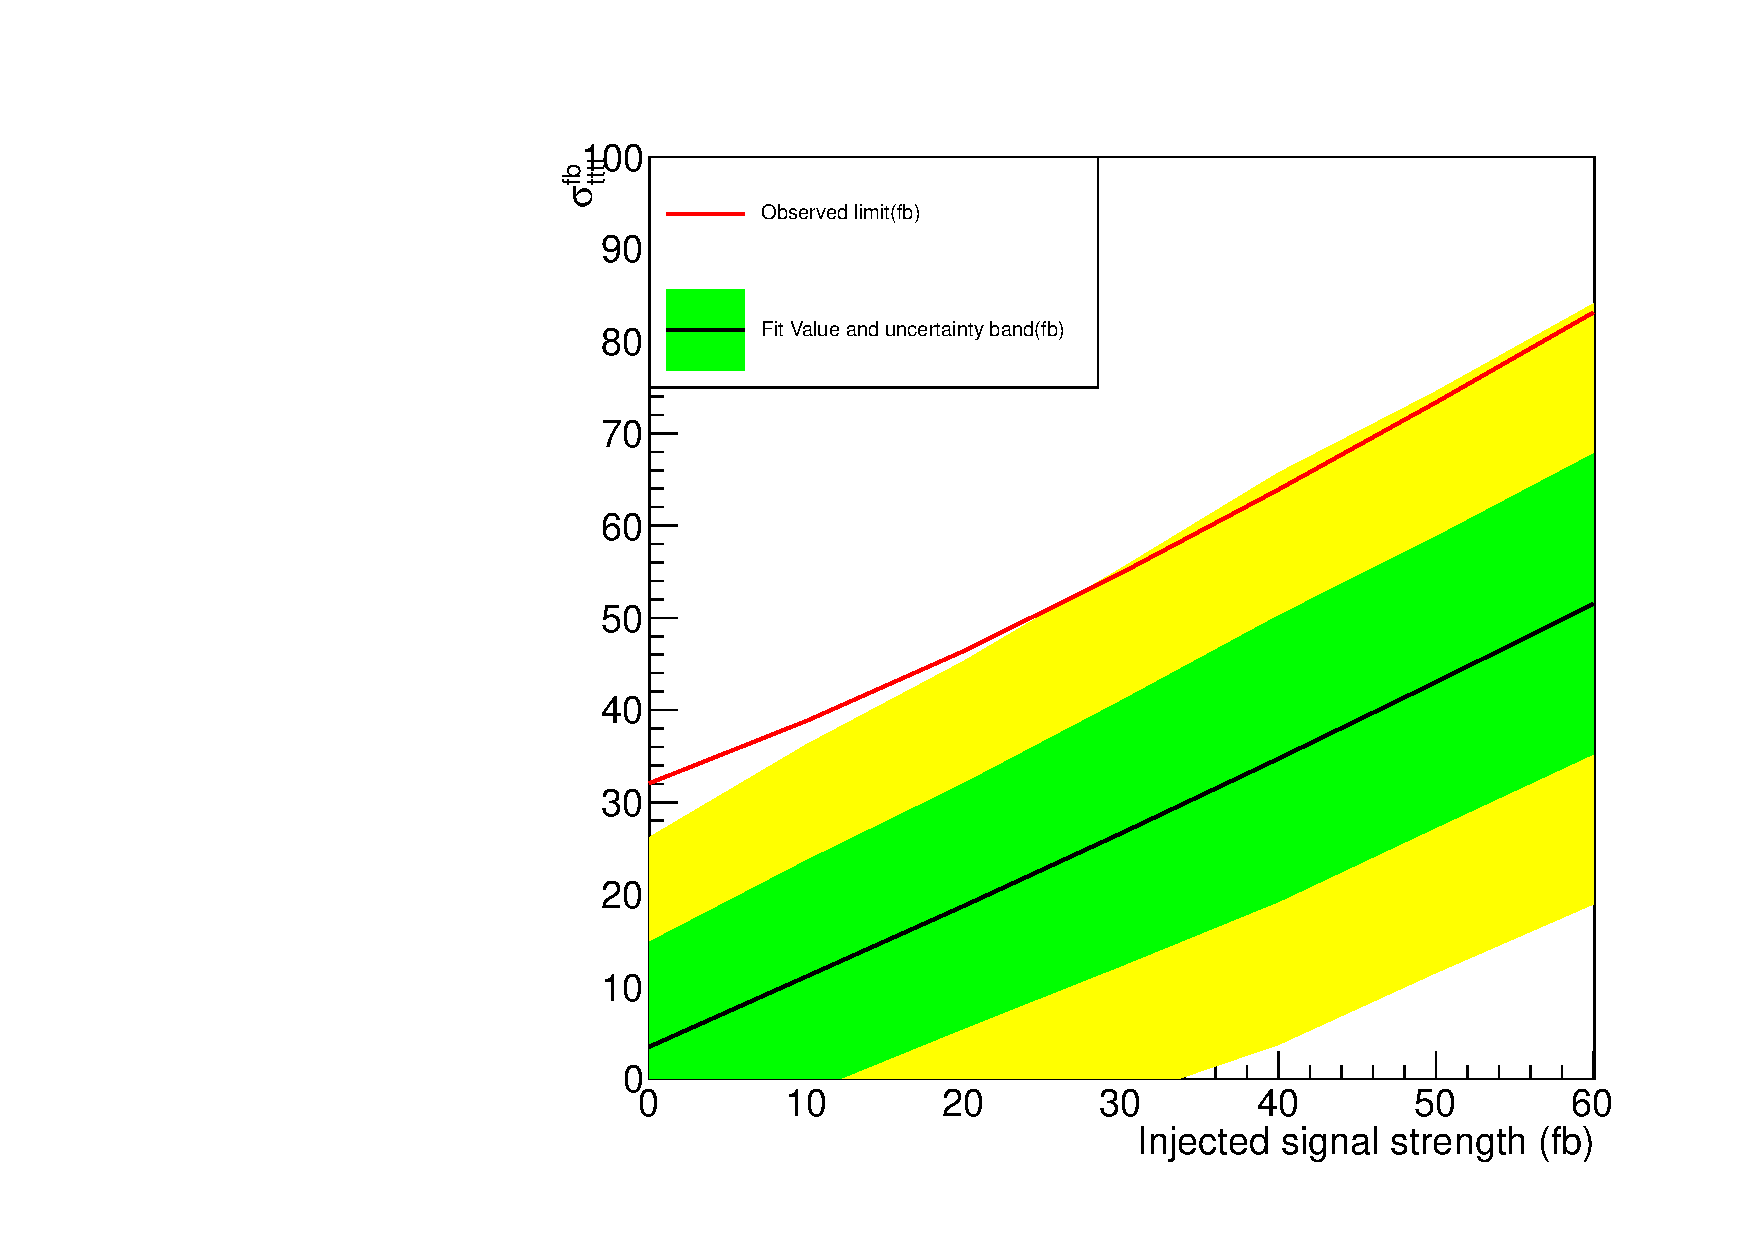
\includegraphics[width=0.6\textwidth]{images/Run1/SignalInjection_JS_Brazil.pdf}
    \caption{Fitted values(fb) and observed(fb) for various injected signal strength(fb).}
    \label{fig:SigInjectionBrazil}
\end{figure}

\section{Summary and conclusion}
\label{sec:summary}

\section{Discussion of ATLAS four-top-quark production studies}
\label{sec:ATLASresult}
\fxnote{Possible comparison with atlas requirements put into our framework}